\documentclass[12pt]{report}
\usepackage{graphicx} % Required for inserting images
\linespread{1.2}

\usepackage[dvipsnames]{xcolor}
\usepackage{tikz}
\usepackage[breakable]{tcolorbox}
\usepackage{colortbl}
\appto{\bibsetup}{\raggedright}

\tikzstyle{mybox} = [draw=BrickRed, fill=BrickRed!5, ultra thick, rectangle, rounded corners, inner sep=10pt, inner ysep=15pt, text width=0.90\textwidth, align=left] 
\tikzstyle{boxtitle} = [fill=BrickRed, text=Apricot!20, ultra thick, rectangle, rounded corners, inner sep=10pt, inner ysep=8pt, text width=0.90\textwidth]

\newcommand{\BoxDef}[2]{%
\vspace*{10px}
\noindent

\begin{center}
\begin{tikzpicture}
    \node[mybox](box){\rule{0pt}{30pt}\ignorespaces#2\unskip};
    \node[boxtitle, anchor=north west] at (box.north west) {\textbf{#1}};
\end{tikzpicture}
\end{center}
}

\newcommand{\colorred}[1]{\textcolor{BrickRed}{#1}}
\newcommand{\colorgreen}[1]{\textcolor{OliveGreen}{#1}}

\newcommand{\ceil}[1]{\left\lceil#1\right\rceil}

\usepackage[]{hyperref}
\usepackage{amssymb}
\usepackage{amsmath}
\usepackage{bm}
\usepackage[top=2.5cm, bottom=2.5cm, left=3cm, right=3cm, centering]{geometry}
\usepackage{algorithm}
\usepackage{algpseudocode}
\usepackage{tabularx}
\usepackage{tabularray}

\begin{document}

\begin{titlepage}
\hrule
\vspace{15pt}
\begin{center}
    \Huge{\textbf{\Huge \textbf{Advanced Databases 23-24}} \\ Notes}\\
\end{center}
\vspace{15pt}
\hrule
\vfill
\hrule
\begin{center}
    \Large University of Pisa \\ M.Sc. in Computer Science
\end{center}
\end{titlepage}

\tableofcontents

\chapter{Introduction}

The most common use of information technology is to store and retrieve data, be it text, images, video, or audio files. As the amount of data generated by several processes increases as time goes on, storage systems must evolve to guarantee reliable access to the data, as well as fast and efficient retrieval. Data is typically stored into \textbf{databases} (\textbf{DBs}), which are housed in a permanent memory.

The technology on which permanent memory is based uses magnetic \textbf{disks}, containing a set of platters that rotate at relatively slow speeds (compared to CPU speed), which can be interacted with by using heads attached to moving arms. Each platter has on both surfaces a set of rings, called \textbf{tracks}, which, except for the innermost and outermost ones, are used to store information. Each track is subdivided into \textbf{sectors} of the same size, which correspond to the smallest unit of transfer allowed by the hardware. Typical sector sizes are 512 bytes, 1 KB, 2 KB, or 4 KB. There are from 500 to 1000 sectors per track, and about 100K tracks per surface of a single platter.

The \textbf{access time} needed to read a section of the disk is given by the seek time (needed to move the head), the rotational delay (given by the spinning of the disk itself), and the transfer time (needed to read/write the data). These operations take several milliseconds to be completed, which are definitely slower than any operation relative to the \textbf{main memory} (\textbf{RAM}), taking only a few nanoseconds in total. 

Despite this disparity, disks are still today the preferred technology to store data. Main memory is, in fact, volatile: once the machine stops receiving electricity powering it on, any information on the RAM is lost forever. On the other hand, disks provide reliable storage: the information written on them can be retrieved even if the machine is turned off and on. A newer technology, called \textbf{solid state storage}, and, in particular, \textbf{flash memory}, has risen in popularity in the last years. It provides the reliability of disks and much faster operations, although they still haven't become the new standard since they tend to be expensive.
\chapter{Overview of a DBMS}

This chapter will give a general overview of the structure of a centralized \textbf{DBMS} (\textbf{Data Base Management System}) based on the relational data model, describing its components and their respective functionalities.

\section{Architecture}

A database is a collection of homogeneous sets of data, with relationships defined among them, stored in permanent memory, and used via a DBMS.

\BoxDef{DBMS}{
A DBMS is a software that provides the following functionalities:
\begin{itemize}
    \item A language to describe the \textbf{schema} of the database (a collection of definitions that describe the data structures), restrictions on the allowed data types, and the relationships among data sets;
    \item The data structures for storage and efficient retrieval of large amounts of data;
    \item A language to guarantee secure access to the data only to authorized users;
    \item A \textbf{transactions} mechanism to protect data from HW/SW malfunctions and errors during concurrent access.
\end{itemize}
}

The architecture of a DBMS provides the following basic components:
\begin{itemize}
    \item The \textbf{Storage Engine}, which includes modules supporting:
    \begin{itemize}
        \item \textbf{Permanent Memory Manager};
        \item \textbf{Buffer Manager};
        \item \textbf{Storage Structures Manager};
        \item \textbf{Access Methods Manager};
        \item \textbf{Transaction and Recovery Manager};
        \item \textbf{Concurrency Manager}.
    \end{itemize}

    \item The \textbf{Relational Engine}, which includes modules supporting:
    \begin{itemize}
        \item \textbf{Data Definition Language};
        \item \textbf{Query Manager};
        \item \textbf{Catalog Manager}.
    \end{itemize}
\end{itemize}
In real systems the functionalities of these modules are not completely separated in different components (as in Figure \ref{fig:DBMS_schema}), but this overview can help in understanding the purpose of each of them. 

\begin{figure}[ht]
    \centering
    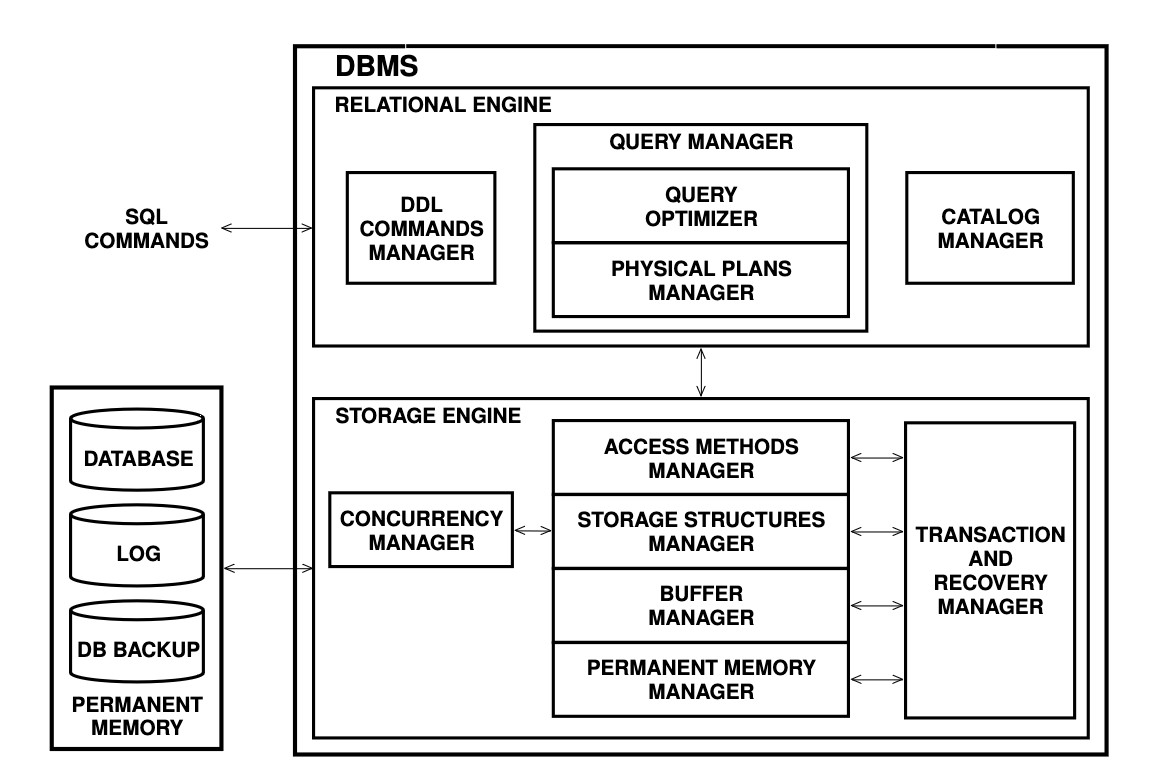
\includegraphics[width=0.75\linewidth]{img/DBMS schema.png}
    \caption{The architecture of a DBMS.}
    \label{fig:DBMS_schema}
\end{figure}

\subsection{Permanent Memory Manager}

The PMM manages page allocation and deallocation on disk storage. It hides the disk characteristics and the operating system, as it provides an abstraction of the memory as a set of databases, each consisting of a set of logical files of \textbf{physical pages} (or blocks) of fixed size. The physical pages of a file are numbered consecutively starting from 0, and their number can grow dynamically with the only limitation being the available space in the permanent memory. Each collection of records (table or index) of a database is stored in a logical file, which can also be realized as an actual separate file of the operating system or as part of a file in which the database is stored.

Once a physical page is transferred to main memory, it is called a \textbf{page}, and it is represented with a specific, complex structure.

\subsection{Buffer Manager}

The Buffer Manager is tasked with transferring pages between temporary and permanent memory. It allows transactions to get the pages they need minimizing the number of disk accesses. In general, the performance of operations on a database depends on the number of pages transferred to temporary memory. If a big enough buffer is used, and there's a high number of access requests for a specific page, there's a high likelihood that such page will be in the buffer. Figure \ref{fig:buffermanager} illustrates the basic structure of a Buffer Manager.

\begin{figure}[ht]
    \centering
    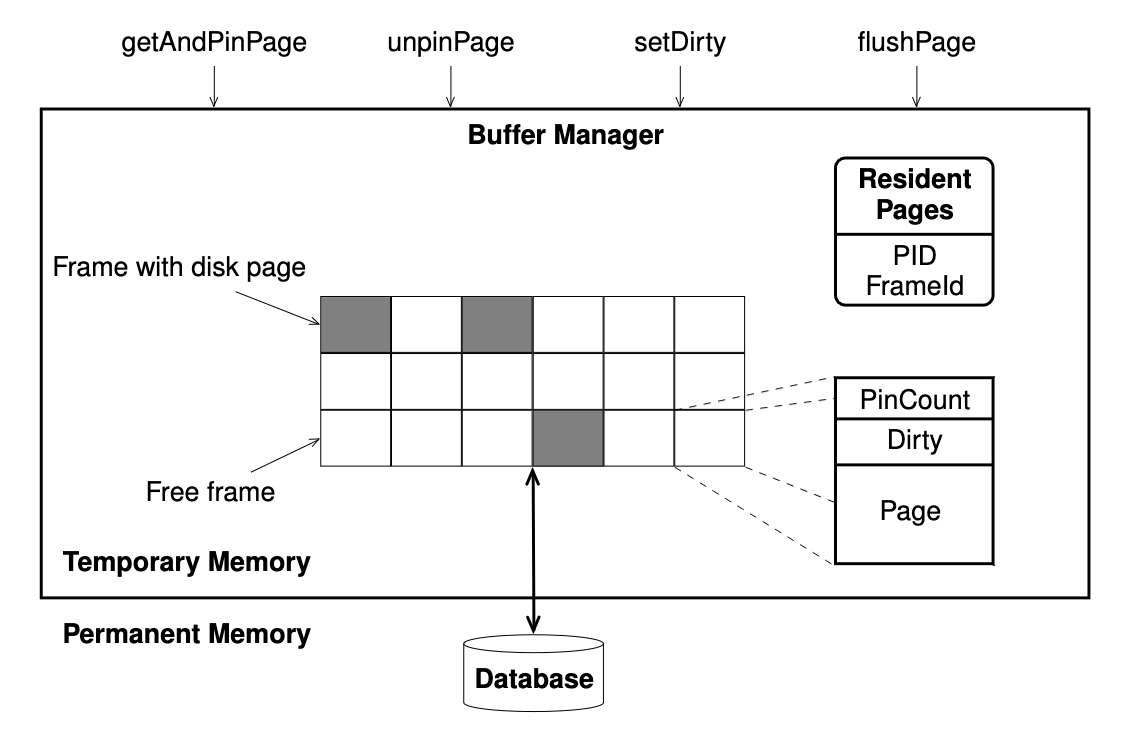
\includegraphics[width=0.5\linewidth]{img/Buffer Manager.png}
    \caption{The components of the Buffer Manager.}
    \label{fig:buffermanager}
\end{figure}

The \textbf{buffer pool} is an array of \textbf{frames}, each containing a copy of a page present in permanent memory, and some additional bookkeeping information. The pool has a fixed size, so when there are no more free frames, a page must be freed with an appropriate algorithm. Each frame stores two variables, the \textbf{pin count} and the \textbf{dirty}. The former counts the number of transactions currently using the page hosted on that frame; its value starts at 0, and increases by 1 each time it is requested, and decreases by 1 each time it is released. The latter indicates whether the page was modified since it was copied into the buffer, signaling that the modification must be reflected on disk as well. The \textbf{resident pages} table is a hash table that is used to know which page in permanent memory (identified by a PID) is stored in which frame.

A commonly used replacement policy is the \textbf{Least Recently Used} (\textbf{LRU}) policy. Once the buffer pool is full, the frame chosen to be ejected is the one that was the earliest one to be pinned. The idea is that since the page hasn't been requested for a relatively long time, it probably won't be requested any time soon. However, this policy may not always be the best: for example, in a join loop between two tables, the LRU policy may be optimal for one table, while the optimal one for the other is Most Recently Used (MRU).

\subsection{Storage Structures Manager}

The Storage Structure Manager implements databases as tables of records, representing the files of pages provided by the Permanent Memory Manager. Above the Storage Structure Manager, the unit of access is a record; below, the unit of access is a page. For this reason, the unit of costs considered for now will be a single page access (read or write), and we assume that memory operations have 0 cost, since they're so much faster than disk operations their addition to the overall cost is negligible. The most important type of file is the \textbf{heap file}, which stores records in no particular order.

A \textbf{record} is a collection of one or more \textbf{attributes}, and contains some extra information, called \textbf{record header}, needed for record management. We assume records are not larger than a page (a few KB big), and that each attribute is either separated from the others using a separator, or all attributes are stored sequentially and are indexed by using an offset. Each record is uniquely identified by a \textbf{RID}, which specifies the page and the offset the record can be found at. Sometimes this offset may be logical, i.e., it actually indicates a position on an array of actual pointers to records; this way, records can be moved around without having to externally modify their RID.

Collections of pages may be stored using different data structures. Usually, pages are stored with two alternatives. The first uses two doubly linked list, one containing free pages, the other containing full ones. The other alternative consists in a \textbf{directory}, where each entry contains a pair PID-available space. If the directory grows and cannot be stored in the header page of the file, it is organized as a linked list. For efficiency reasons, the free space existing in different spaces cannot be compacted into new free pages. If the available free space is plenty but there's no actual free pages available, it may be necessary to reorganize the database.

\section{External Sorting}

A frequent operation done in DBMS is \textbf{sorting}. Sorting collections of records may be done for different reasons: it may be needed to perform a join operation, delete duplicates, or load them into physical organizations.

Since typically temporary memory cannot hold all the records of a file at the same time, merging is done by using \textbf{external sorting algorithms}, of which most widely used one is \textbf{merge-sort}. Let $N_{pag}(R)$ be the number of pages in the file, and $B$ the number of available pages on the buffer. Merge-sort operates in two phases:
\begin{enumerate}
    \item The \textbf{sort phase}, in which $B$ pages are read into the buffer, sorted, and written to disk. This creates exactly $n = \ceil{N_{pag}(R) / B}$ sorted subsets of records, called \textbf{runs}. Each run is stored in a separate numbered auxiliary file, and contains the same number of pages (except for the last one, which may contain less if the number of file pages isn't divisible by the number of free buffer pages);

    \item The \textbf{merge phase}, which fuses the sorted runs to reconstruct the file. In each merge pass, $Z = B-1$ runs are merged using one buffer page left free to produce the output. The number of runs at the end of a merge pass becomes $n = \ceil{n/Z}$. Merges are repeated until $n < 1$.
\end{enumerate}
Once the algorithm terminates, the final auxiliary file contains the sorted data. $Z$ is called the \textbf{merge order}, and a total of $Z + 1$ buffer pages are needed to execute a $Z$-merge (since as stated above, one page must be left free).

The cost of the algorithm is evaluated in terms of how many read/write operations are needed in total, since we're ignoring operations directly involving records. The overall cost is given by two terms:
\begin{align*}
    C_{sort}(R) = SortCost + MergeCost = \\
    = 2 \times N_{pag}(R) + 2 \times N_{pag}(R) \times MergePasses
\end{align*}
If the number of file pages is less than $B^2$, (or, more precisely, $B(B-1)$), the data can be sorted in a single pass, so the cost becomes:
\begin{equation*}
    C_{sort} = 2 \times N_{pag}(R) + 2 \times N_{pag}(R) \times 1 = 4 \times N_{pag}(R)
\end{equation*}
The number of passes is a function of the number of file pages $N_{pag}(R)$, the number of initial runs $S$, and $Z$. $S$ also depends on the number of file pages and the number of buffer pages available at the start:
\begin{equation*}
    S = \ceil{N_{pag}/B}
\end{equation*}
At each merge pass, the algorithm merges together $Z$ runs. At the start, the runs will be $S$. After one merge pass, they will be $S/Z$. At the second pass, they will be $S/Z * 1/Z = S/Z^2$, and so on until only one run remains. Since the number of runs decreases exponentially, we can write that the total number of passes will be:
\begin{equation*}
    k = \ceil{\log_Z{S}}
\end{equation*}
The total cost can be rewritten as:
\begin{equation*}
    C_{sort} = 2 \times N_{pag}(R) + 2 \times N_{pag}(R) \times \ceil{\log_Z(S)} \ .
\end{equation*}

\section{Data Organizations}

\subsection{Heap and Sequential Organizations}

The data can be arranged either via \textbf{heap organization}, or \textbf{sequential organization}. With heap organization, every new record is added to the end of the file: insertion is easy and efficient in terms of memory used. It is ideal for situations where insertion is more common than search, or files where massive search is common. This is also the standard organization for DBMS.

With sequential organization, data is kept sorted on a \textbf{search key} $K$, picked as a single attribute of the records. This makes equality and range search on $K$ very efficient. On the other hand, insertion is more problematic, since the ordering of the records must be maintained at all times. Insertion may use a \textbf{static solution}, where each page is filled normally, and for each insertion, the record is placed at the correct spot in the ordering, moving all other records after it. A \textbf{dynamic solution} instead keeps some fraction of the total space in a page free. Once a page has filled up enough, its contents are split into new pages. This way, pages always have some extra space at the end to accommodate new insertions: when a record is added, the shifting of the records after it will only involve the ones in the same page. Alternatively, a \textbf{differential file} may be used to keep track of which changes must be applied to which pages, so that all insertions can be done all at once in a second moment.

Table \ref{tab:heap-seq-comp} shows a comparison between the two organization types. $N_{pag}(R)$ refers to the number of pages required to store the records. The \textbf{selectivity factor} $sf$ is an estimate of the fraction of pages occupied by records that satisfy the condition of a range search, and is calculated as:
\begin{equation*}
    sf = \dfrac{(k_2 - k_1)}{(k_{max} - k_{min})} \ ,
\end{equation*}
with $k_1$ and $k_2$ being the two extremes of the range, and $k_{max}$ and $k_{min}$ the highest and lowest values in the domain of the attribute.

\begin{table}[ht]
\small
\centering
\SetTblrInner{rowsep=5pt}
\begin{tblr}{hlines, vlines, columns={75pt, c, m}, column{1}={50pt, c}, column{2}={50pt, c}, column{5}={50pt,c}, column{6}={50pt, c}}
        \textbf{Type} & \textbf{Memory} & \textbf{Eq. Search} ($C_s$) & \textbf{Range Search} & \textbf{Insertion} & \textbf{Deletion} \\
\hline
        \textbf{Heap} & $N_{pag}(R)$ & $\ceil{\dfrac{N_{pag}(R)}{2}}$ & $N_{pag}(R)$ & $2$ & $C_s + 1$ \\

        \textbf{Seq.} & $N_{pag}(R)$ & $\ceil{\log_2{N_{pag}(R)}}$ & $C_s - 1 + \ceil{sf \times N_{pag}(R)}$ & $C_s + 1$ $+ N_{pag}(R)$ & $C_s + 1$ \\

\end{tblr}
    \caption{Comparison between heap and sequential organization.}
    \label{tab:heap-seq-comp}
\end{table}

The equality search is faster for the sequential one since it uses a binary search algorithm, while the heap one has to compare the record against all pages since no specific ordering is imposed. The cost estimation is also only valid if the data distribution is uniform; if it follows some other distribution, e.g., Gaussian, the actual cost may be high (worst case exactly $N_{pag}(R)$).

The range search for the heap organization costs $N_{pag}(R)$ since it must read all pages to make sure it collects all records falling within the specified range. For sequential organization, it costs an equality search to find the starting record of the range, plus the number of pages needed to store the records in that range. The ``$-1$'' is added because the first page has already been found with the binary search.

The final biggest difference lies in the costs for insertions: it is constant for heap organization, while for sequential organization it costs a search to find the spot to insert the record, and all subsequent $N_{pag}/2$ pages must be read and written to move their records forward. If the page the record is added to is not completely full, the insertion will still cost $C_s + 1$.

\subsection{Key-based Organizations}

A table organization based on a key allows the retrieval of a record with a specified key in as few accesses as possible, 1 being the optimum. The set of records in the table is \textbf{mapped} to a set of keys, via either a \textbf{primary organization} or a \textbf{secondary organization}.
\BoxDef{Primary and Secondary Organizations}{
A table organization is primary if it determines the way the records are physically stored, and therefore how they can be retrieved. Otherwise, it is a secondary organization.
}
For a primary organization, the mapping can be done using a \textbf{hash function} or a \textbf{tree structure}. It can be either \textbf{static} or \textbf{dynamic}.
\BoxDef{Static and Dynamic Primary Organization}{
A primary organization is static if the performance degrades gradually as insertions and deletions are performed, requiring reorganization. \\
A primary organization is dynamic if once created, it evolves with insertions and deletions, preserving efficiency of operations.
}
In a secondary organization, the mapping from key to record is implemented with the \textbf{tabular method}/\textbf{index}, listing all inputs and outputs.

\subsubsection{Static Hashing Organization}

This is the simplest methods for a primary table organization. We assume to have $N$ records all of the same fixed size, and that keys are integers. The records of the same table $R$ are stored in the \textbf{primary area}, divided into $M$ buckets, each of which may consist of one or several pages. For now, we will assume each bucket to contain only one page of capacity $c$, and that pages are numbered from $0$ to $M-1$.

A record is inserted into a specific bucket chosen by calculating its address via a \textbf{hashing function} $H$, applied to the record key value. The ratio:
\begin{equation*}
    d = \dfrac{N}{(M \times c)}
\end{equation*}
is called the primary area \textbf{loading factor}, which represents how full the primary area is. The hash function should produce addresses uniformly distributed in the interval $[0, M-1]$, and it may return the same address for different keys. This causes a \textbf{collision}. Records hashed to the same page are stored in order of insertion. When an insertion is attempted in a page that is completely full, an \textbf{overflow} occurs, and must be appropriately managed.

The design of a static hashing organization depends on the choices done for the following parameters:
\begin{enumerate}
    \item The \textbf{hashing function}: a good hashing function must randomly assign keys to elements in the address space. There's no single ``ideal'' hash function, but generally, simpler functions tend to perform better than complex ones. A common choice is the \textbf{modulo function}: $H(k) = k \mod M$, with $M$ a prime number.

    \item The \textbf{overflow management technique}: two commonly used techniques are \textbf{open overflow} and \textbf{chained overflow}. Open overflow performs a primary area linear search to find the first empty space to insert the record; when the last page has been searched, the process restarts from the initial page. Chained overflow collects overflow records chained together in a separate area, pointed to from the home page.

    \item The \textbf{loading factor}: low loading factors and higher page capacities give better performances, but occupy more memory. For low ($d < 0.7$) loading factors, retrieving a record requires a single access on average. For high values ($d > 0.8$), the primary area size is reduced, increasing the probability of overflow; open overflow deteriorates rapidly, while chained overflow still performs well.  

    \item The \textbf{page capacity}: higher values of page capacity reduce the number of overflows, which are the main culprit in performance degradation of hashing organizations.
\end{enumerate}
As for overall performances, for page capacities less than 10 it is preferable to give up hash organizations. A static hashing has excellent performances as long as there are no overflows to manage, with the average cost of an equality search being 1. As overflows start to happen, reorganization is needed, which requires the creation of a new primary area, choosing a new hash function, and reloading all the data.

A big drawback of static hashing is that is does not support efficient range queries, since records with similar keys will typically not end up in the same bucket.

\subsubsection{Dynamic Hashing Organization}

Dynamic hashing organizations can be divided into two groups: those that use a primary area and an auxiliary data structure whose size changes with the primary area size, and those in which only the primary area size changes dynamically. In both cases, the hashing function changes automatically when the structure changes dimension, maintaining the average access time equal to 1. We will see two types of dynamic organizations with auxiliary data structures (Virtual Hashing and Extendible Hashing), and two without (Linear Hashing and Spiral Hashing).

\paragraph{Virtual Hashing}

Virtual hashing works as follows:
\begin{enumerate}
    \item The data area initially contains $M$ contiguous pages of capacity $c$. Each page is identified by its address (between $0$ and $M-1$).

    \item A bit vector $\mathcal{B}$ is created, indicating with a $1$ which page contains at least a record.

    \item An initial function $H_0$ is used to map each key to and address $m$. If an overflow happens, then the data area is doubled, maintaining the pages as contiguous, the hashing function is replaced with a new one ($H_1$) that maps keys to addresses in the range $[0, 2M-1]$, and the hashing function is applied to all keys and all records in the overflowing page $m$. These records end up being distributed between $m$ itself and some other new page $m'$.
\end{enumerate}
This method defines a series of hashing functions,
\begin{equation*}
    H_0, H_1, H_2, \dots, H_r \ ,
\end{equation*}
where $H_i$ produces a page address in the range $[0, 2^i M-1]$. The function chosen as the hash function must satisfy the following constraints:
\begin{align*}
    &H_{j+1}(k) = H_j(k) \\
    \text{or}\\
    &H_{j+1}(k) = H_j(k) + 2^j \times M ,\ j=r,r-1,\dots,0
\end{align*}
for all keys $k$. This means that the new hash function chosen either returns the same address the key already corresponds to, or a new address that is equal to the original one plus half of the new address space. A common function is $H_r(k) = k \mod (2^r \times M)$.

To find a record, known its key and $r$ (the number of times the data area has been doubled), a recursive function is used:
\begin{algorithm}[ht]
\caption{PageSearch pseudocode.}
\begin{algorithmic}[1]
    \If{$r < 0$}
        \State The key does not exist.
    \ElsIf{$\mathcal{B}(H_r(k)) == 1$}
        \State Return $H_r(k)$
    \Else
        \State PageSearch($r-1$, $k$)
    \EndIf
\end{algorithmic}
\end{algorithm}
This technique requires memory equal to the one occupied by the data area and the bit vector $\mathcal{B}$. The memory is not very well used however, because of the frequent need to double the data area.

\paragraph{Extendible Hashing}

Instead of using a bit vector, extendible hashing uses a fixed set of data pages with a \textbf{directory} $\mathcal{B}$, containing a set of pointers to data pages. The directory is smaller in size than the primary area, and is doubled as needed.

Let $r$ be a record with key $k$. The value produced by $H(k)$ is a binary value of $b$ bits (usually 32), called hash key. The hash key does not represent an actual address; instead, pages are allocated on demand as records are inserted into the file, considering only the initial $p$ bits of $b$, which are used as an offset into the directory $\mathcal{B}$. The value of $p$ grows and shrinks with the number of pages used by data, and the number of entries in the directory is always $2^p$. $p$ is called the \textbf{directory level}. Each entry in the directory is a pointer to a data page containing records with the same first $p'$ bits of their hash key, with $p' \in [0, p]$. $p'$ is called \textbf{data page level}.

The hash structure is initially empty, with $p=0$, and is a directory with one entry containing a pointer to an empty page of capacity $c$. The first $c$ records are inserted in the page; as we try to insert a new record into a full page, there are two possibilities:
\begin{itemize}
    \item If $p' = p$, $\mathcal{B}$ is doubled and $p$ becomes $p+1$. Let $w$ be the bits of the previous value of $p$. Then, the entries in the doubled directory indexed by $w0$ and $w1$ each contain a pointer to the same data page that $w$ used to point to.

    \item If $p' < p$, then the data page is split in two, creating a new page, and each of the halves' level $p'$ take value $p'+1$. The records in the original page are distributed across the halves, based on the value of the first high-order bit of their hash keys. Records whose key has 0 in the $(p'+1)^{th}$ bit stay in the old page, while those with a 1 will go in the new one. The pointers in the directory are updated so that those that pointed to the original page now point to the new half, depending on the value of the $(p'+1)^{th}$ bit.
\end{itemize}
The advantage of this method is that performance does not degrade as the file grows, and the directory $\mathcal{B}$ keeps the memory overhead low. The retrieval of a record has an additional level of indirection since $\mathcal{B}$ must be accessed first, but this has very little impact on the performance, since most of the directory will be in main memory.

\paragraph{Linear Hashing}

Linear hashing increases the number of data pages as soon as an overflow occurs, but the page which is split is not the one that flows over; instead, it is the page pointed by the current pointer $p$, initially equal to 0, and incremented to 1 each time an overflow happens.

Initially, $M$ pages are allocated, and the hash function used is $H_0(k) = k \mod M$. When an overflow happens in a page with address $m \geq p$, an overflow chain is maintained for page $m$, and a new page is also added. All records in page $p$ are distributed between page $p$ and the new page, using the new hash function $H_1(k) = k \mod 2M$.

As page $M$ overflows, a total of $M$ duplications have happened, bringing the memory to $2M$ pages. Pointer $p$ is reset, and $H_0$ is replaced by $H_1$. $H_1$ is in turn replaced by $H_2(k) = k \mod 2^2 M$, and so on. After $r$ doublings, the function $H_r(k) = k \mod 2^r M$ will be used. To retrieve a record with key value $k$, the page address is calculated as:
\begin{algorithm}
\caption{PageAddress pseudocode.}
\begin{algorithmic}[1]
    \If{$H_i(k) < p$}
        \State $H_{i+1}(k)$
    \Else  
        \State $H_i(k)$
    \EndIf
\end{algorithmic}
\end{algorithm}
\\Linear hashing has similar performances to extendible hashing.

\paragraph{Spiral Hashing}

Spiral hashing considers the memory as if it were organized on a spiral instead of a line. Like linear hashing, spiral hashing requires no index, but has better performances and storage utilization because of three particular property:
the hashing function distributes records unevenly, accumulating records in the pages at the beginning of the address space, while the pages at the end have a lower load. The page that is split is one that is very unlikely to overflow.

\subsubsection{Tree-structure Organizations}

All the previous organizations have the big disadvantage of not supporting the range equality search operation. An alternative organization commonly used in DBMSs use dynamic tree structures to store pages. The \textbf{order} of a tree is the maximum number of children a node can have. The \textbf{level} of a node is the number of nodes encountered in the path from the root to the node itself. The \textbf{height} of the tree is the maximum level of a node. A tree is \textbf{balanced} if the levels of all leaf nodes differ by at most 1.

The types of trees most commonly used are B-trees and B$^+$-trees, since unlike binary trees they manage to keep a relatively low height even with a high number of pages. One solution may be to store the nodes of the binary tree in main memory, such that each page contains the same number of nodes. In the example shown in Figure \ref{fig:paged-bintree}, each page contains 8 nodes, each of which refers to 8 different pages. Using this strategy, the depth of the tree in terms of pages to access is greatly reduced: an equality search has a complexity of $\log_8 (N_{pag}(R))$ instead of $\log_2 (N_{pag}(R))$.

\begin{figure}[h!]
    \centering
    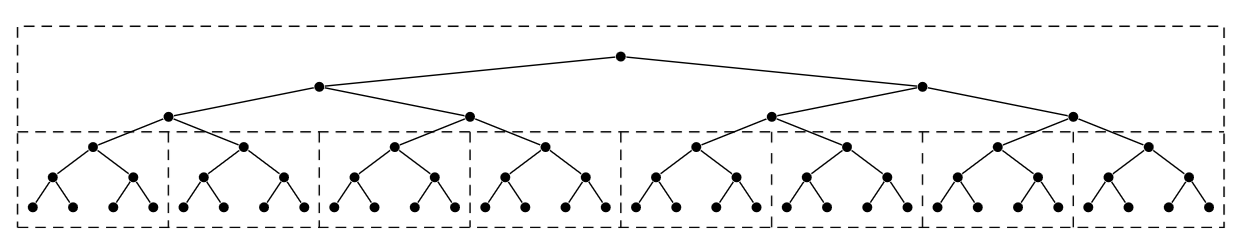
\includegraphics[width=1.0\linewidth]{img/paged_bintree.png}
    \caption{A paged binary tree: each page in main memory is delimited by a dashed line.}
    \label{fig:paged-bintree}
\end{figure}

Still, this structure must be kept balanced when insertions or deletions are performed, and algorithms that maintain binary trees can be very costly. The following sections will explain how using multiway trees can be a solution.

\paragraph{B-trees}

A B-tree is a perfectly balanced search tree, in which each node has a variable number of children. We will indicate a key as $k$ and the full record associated with it $k*$. Also, we'll assume that all keys are integers and that all records have the same fixed size. An example of B-tree can be seen in Figure \ref{fig:B-tree}.

\begin{figure}[ht]
    \centering
    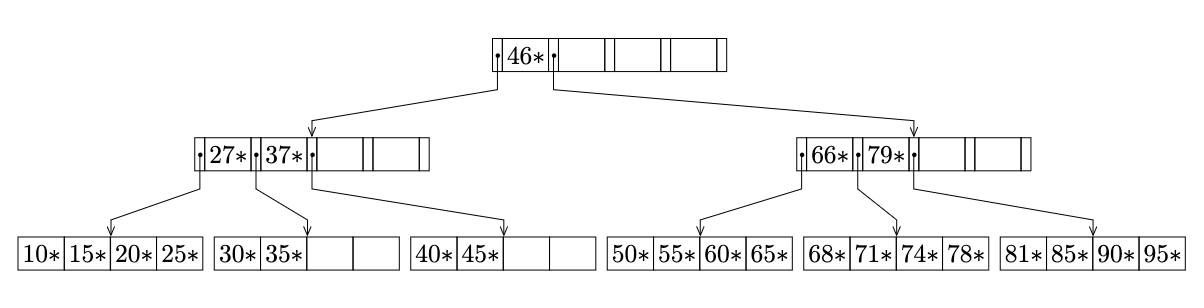
\includegraphics[width=1.0\linewidth]{img/B-tree.png}
    \caption{A B-tree.}
    \label{fig:B-tree}
\end{figure}
A B-tree is defined as follows:
\BoxDef{B-tree}{
A B-tree of order $m \geq 3$ is an $m$-way search tree that is either empty or of height $h \geq 1$, and satisfies the following properties:
\begin{itemize}
    \item Each node has at most $m - 1$ keys, and, except for the root, at least $\ceil{m/2} - 1$ keys;

    \item A node with $j$ keys will have $j+1$ pointers to children, undefined in the leaves, and $K(p_i)$ is the set of all keys in the $i^{th}$ child node;

    \item All leaves are on the same level;

    \item Each non-leaf node has the same following structure:
    \begin{equation*}
        [p_0, k_1*, p_1, k_2*, \dots, k_j*, p_j] \,,
    \end{equation*}
    where each $p_i$ is a pointer to a child node such that, for all $0 < i < j$:
    \begin{align*}
        &\forall k \in K(p_i), \ k_{i} < k < k_{i+1}
    \end{align*}
\end{itemize}
}
There is a strict relationship between the height of the tree $h$, the order $m$, and the number of keys $N$. Since the non-root nodes are constrained in the number of keys they must maintain, the following inequality holds true:
\begin{equation*}
    \log_m (N+1) \leq h \leq \log_{\ceil{m/2}}(\dfrac{N+1}{2}) + 1
\end{equation*}
The left size of the inequality corresponds to a B-tree with all of its nodes completely filled, while the right side to a B-tree where each node has the least acceptable amount of keys.

The following is a summary of the costs of operations using a B-tree. An equality search for a specific key $k$ starts at the root; if the key is not in the root (and $h > 1$), the search continues in the child that will likely contain the key (since keys are ordered, the chosen pointer is the one right after the biggest key smaller than $k$). The overall cost is $1 \leq C_s \leq h$.

As for the range search, to retrieve all records with keys in increasing order, the tree must be visited in the \textbf{in-order traversal}, starting from the leftmost leaf and gradually moving to the right. Let $sf = (k_2 - k_1)/(k_{max} - k_{min})$ be the selectivity factor for the search; the overall cost will be $C_{range} = sf \times N_{nodes}$, since keys will be ``scattered'' across different nodes of the tree at different levels. The following bond holds true: $h \leq C_{range} \leq N_{nodes}$. It will always require traveling to a leaf, and in the worst case scenario, it may have to read all nodes in the tree.

Insertion in a non-full leaf is easy: the new key is simply added to a leaf so that the keys are correctly sorted. The cost is $h$ reads and 1 write. If the leaf is full, then the node must be split, so that the old node will retain the first half of keys, and the new node will get the second half. The median key is inserted into the parent node, and the new node is pointed by the pointer on its right. In case the parent node is full as well, the operation repeats. The cost for the worst case scenario is $h$ reads and $2h + 1$ writes.

For deletion, there are three possibilities:
\begin{itemize}
    \item If the key is in a leaf, and the removal keeps the number of keys within the acceptable range, the cost is $h$ reads and 1 write;

    \item If the key is a node, and no other operations are needed, the cost is $h$ reads and 2 writes (the key is replaced with the next following one);

    \item If the key is in a leaf node and the final number of keys is less than $\ceil{m/2} - 1$ elements, then a \textbf{rotation} or a \textbf{merge} are needed.

    A node is merged with one of its brothers which contains $\ceil{m/2} - 1$ keys, moving all of them to the first node. Additionally, the key in the parent node that was between the pointers of the two children involved in the merging is also removed and added to the merged child. In case this produces an underflow in the parent node, the operation is repeated until the whole tree is balanced.

    When a merge is not possible because all brothers are too full, a rotation is performed instead. When the key is deleted, the maximum key from the left brother is moved into the parent, and the key in the parent is moved into the underfull node.

    When either of these operations are needed for all nodes from root to leaf, the cost is $2h - 1$ reads and $h + 1$ writes.
\end{itemize}
Table \ref{tab:B-tree-comp} summarizes all the operation costs.

\begin{table}[ht]
\small
\centering
\SetTblrInner{rowsep=5pt}
\begin{tblr}{hlines, vlines, columns={80pt, c, m}, column{1}={60pt}}
    & \textbf{Eq. Search} ($C_s$) & \textbf{Range Search} & \textbf{Insertion} & \textbf{Deletion} \\
\hline
    Best case & 1 & $sf \times N_{nodes} = h$ & $h + 1$ & $h + 1$ or $(h + 2)$ \\     
    Worst case & $h$ & $sf \times N_{nodes} = N_{nodes}$ & $2h + 1$ & $(2h - 1) + (h + 1)$ \\
\end{tblr}
    \caption{Costs for B-tree organization.}
    \label{tab:B-tree-comp}
\end{table}

\paragraph{B$^+$-trees}

B$^+$-trees are a variant of B-trees that perform especially well for range searches. In a B$^+$-tree, all the records $k*$ are stored sorted in the leaf nodes, organized in a doubly linked list. Each non-leaf node stores the highest key of the child pointed by the previous pointer. An example of B$^+$-tree can be seen in Figure \ref{fig:B+-tree}.

\begin{figure}[ht]
    \centering
    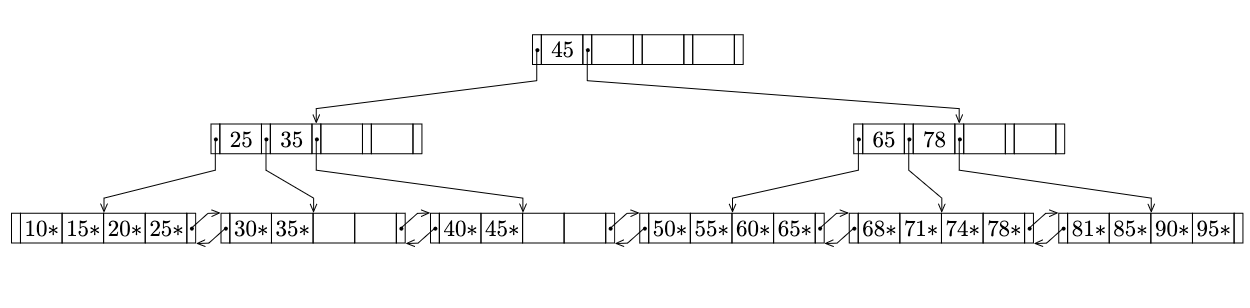
\includegraphics[width=1\linewidth]{img/B+-tree.png}
    \caption{A B$^+$-tree.}
    \label{fig:B+-tree}
\end{figure}
It can be thought of as the combination of a sparse index and a sequential file. Records are part of the tree structure stored in one file, so to read all records in a sorted order, the tree structure must be necessarily used to locate the first data page.

Compared to B-trees, B$^+$-trees tend to be much shallower, since the non-leaf nodes only contain keys but not records, which can be found in the leaves, connected together. This makes any sequential/range scan of the data faster: the cost for a ranged search is $sf \times N_{leaves}$. For the equality search, since we're assuming the tree to have a level equal to no more than 3, will take from 1 to 3 read operations.

Another big difference is that in deletion, there's no need to replace it in the father node, unless the deletion requires a merge or rotation (in which case the operations are the same as the B-tree).

\subsubsection{Index (Secondary) Organizations}

A secondary organization is defined as follows:
\BoxDef{Secondary Organization}{
An index $I$ on a key $K$ of a set of records $R$ is a sorted table $I(K, RID)$ on $K$, where $N_{rec}(R) = N_{rec}(I)$. An element of the index is a pair $(k_i, r_i)$, where $k_i$ is the key of a record, and $r_i$ is the corresponding RID.
}
An index is a tabular data structure that supports fast retrieval of records by exploiting the ordering of the keys. It can be defined on one or more keys. An index is typically stored in a B$^+$-tree structure.

If the order of the data records is approximately the same as the order of the entries in the index, then it is called a \textbf{clustered index}. When the index is first created, a sort is performed on the actual data records, matching the index order. As insertions are performed, this ordering may be gradually lost, also reducing the effectiveness of such organization, so the clustered index may have to be recreated from time to time. If instead the data records do not follow the same order as the index records, it is called an \textbf{unclustered index}.

The cost for searches done using this organization can be broken down into two terms:
\begin{equation*}
    C_s = C_I + C_D \,,
\end{equation*}
where $C_I$ is the cost of accessing the index pages to find the $RID$s needed, and $C_D$ is the cost of accessing the actual data pages containing the records. Table \ref{tab:indexes-comp} summarizes the differences between the two types of indexes.

\begin{table}[ht]
\small
\centering
\SetTblrInner{rowsep=5pt}
\begin{tblr}{hlines, vlines, columns={80pt, c, m}}
    & \textbf{Eq. Search} ($C_s$) & \textbf{Range Search} \\
\hline
    Clustered & $C_I = 1$, $C_D = 1$ & $C_I = sf \times N_{leaf}$, $C_D = sf \times N_{pag}$ \\     
    Unclustered & $C_I = 1$, $C_D = 1$ & $C_I = sf \times N_{leaf}$, $C_D = sf \times N_{rec}$ \\
\end{tblr}
    \caption{Costs clustered vs. unclustered indexes.}
    \label{tab:indexes-comp}
\end{table}
In ranged search, both types need the same time to retrieve the relevant indexes: either way, they are always sorted by key and easily accessed since they're all part of the same doubly linked list; we're still assuming that since a B$^+$-tree structure is used, the tree will be pretty shallow. Using clustered indexes, the order in which indexes are found is the same as the order of the actual data on disk: the cost of accessing the data depends only on the number of pages the file is made up of, and we will only have to access $sf$ of them in order. With unclustered indexes, the data is not ordered in the same way as the index. There's no way to know exactly where each record is stored in relation to the pages, so each $RID$ returned by the key retrieval corresponds to an individual page access.

\subsection{Non-Key Attribute Organizations}

Up until now, all operations were done on keys, i.e., attributes that uniquely identify records. In many cases, however, we may be interested in retrieving records based on the values taken by other attributes. For example, imagine a table representing students attending the same school, each uniquely identified by a numeric code, and containing information about their name and age. An operation we may want to find all students within a specific age range, or all students who share the same surname. This section will describe how such operations can be done efficiently.

Specifically, the three types of operations that can be performed on non-key attributes are the equality search, the range search, and the \textbf{boolean search}, which consists in the previous operations combined with boolean logical operators.


\subsubsection{Inverted Indexes}

\BoxDef{Inverted Index}{
An inverted index $Idx$ on a non-key attribute $K$ of a table $R$ is a sorted collection of entries, each in the form
\begin{equation*}
    (k_1, n, p_1, p_2, \dots, p_n) \,,
\end{equation*}
where each value $k_i$ of $K$ is followed by the number of records $n$ with that value, and the \textbf{sorted} RID list of these records.
}

Each entry in the inverted index has variable length, depending on how many records in the table $R$ have the same value for the attribute. Also, RIDs are added or removed as records are added or removed from the table. Despite the need to manage these indexes, they are still widely used, especially for cases in which searches are more common than insertions of deletions.

To evaluate performances, we will introduce these terms: $N_{key}(Idx)$ and $N_{leaf}(Idx)$, which are the number of distinct keys and leaf nodes in the index $Idx$. Also, all estimates are done assuming that index-key values are uniformly distributed, as well as records, and the index organization is a B$^+$-tree with the RID lists stored in the leaves. Each cost will be broken down into $C_I$ and $C_D$, as seen before.

For the equality search, the cost of accessing the index is simply $sf(\psi) \times N_{leaf}(Idx)$, or, alternatively, $\ceil{N_{leaf}(Idx) / N_{key}(Idx)}$. Here, $sf$ is calculated as:
\begin{equation*}
    sf(\psi) = \dfrac{1}{N_{key}(Idx)} \,,
\end{equation*}
since we're assuming uniform distribution of the values. All RIDs can be found close together since the leaves are sorted by key (i.e., the non-key attribute of the original table).

For $C_D$, the cost is different whether the data is sorted or not on the index key, so whether the index is clustered or unclustered. If it is unclusterd, there is no information regarding how the records are ordered in their storage structure, so it may be that for each record, the whole page it is found in must be read. THe number of records to retrieve is estimated as:
\begin{equation*}
    E_{rec} = sf(\psi) \times N_{rec}(R) = \ceil{\dfrac{N_{rec}(R)}{N_{key}(Idx)}}
\end{equation*}
since uniform distribution of the values is assumed.
The cost of retrieving the data is:
\begin{equation*}
    C_D = \ceil{\Phi(E_{rec}, N_{pag}(R))} \,,
\end{equation*}
where $\Phi()$ is called \textbf{Cardenas' formula}, and is estimated as:
\begin{equation*}
    \Phi(k,n) = n(1 - (1 - \dfrac{1}{n})^k) \leq \min(k,n)
\end{equation*}
So, the cost will be less or equal than the smallest term: if there's a lot more records than pages, chances are that a single page may contain multiple relevant records, while if the number of records is lower than that of pages, records will rarely appear together in the same page. If the index is clustered, then the cost is:
\begin{equation*}
    C_D = \ceil{sf(\Psi) \times N_{pag}(R)} 
\end{equation*}
Also, if the RID lists are unsorted, then the cost is always $E_{rec}$.

For the range search, $C_I$ remains the same, except that $sf(\Psi)$ is calculated as the ratio between the interval and the attribute's range. $C_D$ is calculated as the product between the number of index key values, and the number of pages to access to retrieve the records indicated by the RID lists. The first term is $\ceil{sf(\Psi) \times N_{key}(Idx)}$, because we will retrieve a certain number of records for each index key included in the range. The second term again depends on whether the index is clustered or unclustered.

If the index is unclustered, then $C_D$ is estimated as:
\begin{equation*}
    C_D = \ceil{sf(\Psi) \times N_{key}(Idx)} \times \ceil{\Phi(\ceil{\dfrac{N_{rec}(R)}{N_{key}(Idx)}}, N_{pag}(R))} \,,
\end{equation*}
while, if it is clustered, it is:
\begin{equation*}
    C_D = \ceil{sf(\Psi) \times N_{key}(Idx)} \times \ceil{\dfrac{1}{N_{key}(Idx)} \times N_{pag}(R)} = \ceil{sf(\Phi) \times N_{pag}(R)}
\end{equation*}
If the RID lists are unsorted, then the second term is always $\ceil{N_{rec}(R) / N_{key}(Idx)}$.

The summary of performances is shown in Table \ref{tab:inverted-idx}.

\begin{table}[ht]
\small
\centering
\SetTblrInner{rowsep=5pt}
\begin{tblr}{
    hlines,
    vlines,
    columns={160pt, c, m},
    column{1}={80pt}
}
     & \textbf{Eq. Search} & \textbf{Range Search} \\
    \hline
     Sorted RID lists, clustered & $C_I = \ceil{sf(\Psi) \times N_{leaves}(Idx)}$, $C_D = \ceil{sf(\Psi) \times N_{pag}(R)}$ & $C_I = \ceil{sf(\Psi) \times N_{leaves}(Idx)}$, $C_D = \ceil{sf(\Psi) \times N_{pag}(R)}$ \\
     Sorted RID lists, unclustered & $C_I = $ as above, $C_D = \ceil{\Phi(E_{rec}, N_{pag})}$ & $C_I = $ as above, $C_D = \ceil{sf(\Psi) \times N_{key}(Idx)} \times \ceil{\Phi(E_{rec}, N_{pag}(R))}$ \\
     Unsorted RID lists & $C_I = $ as above, $C_D = E_{rec}$ & $C_I = $ as above, $C_D = \ceil{sf(\Psi) \times N_{key}(Idx)} \times E_{rec}$ \\
    
\end{tblr}
\caption{Costs for inverted indexes. $E_{rec}$ is $\ceil{N_{rec}(R)/N_{key(R)}}$}
\label{tab:inverted-idx}
\end{table}

\subsubsection{Bitmap Indexes}

\BoxDef{Bitmap Index}{
A bitmap index $Idx$ on a non-key attribute $K$ of a table $R$ with $N$ records, is a sorted collection of entries in the form $(k_i, B)$, where each $k_i$ of $K$ is followed by a sequence of $N$ bits such that the $j^{th}$ bit is set to 1 if the $j^{th}$ record has value $k_i$ for attribute $K$, 0 otherwise.
}
Bitmap indexes are used in DBMS where data is never updated, such as data warehouses, since operations that modify this type of index can be complex, especially when it's compressed. They can also easily solve multi-attribute queries, since the answer can be found by doing a bit-wise AND between two or more bitmaps.

Indicating with $L_k$ and $L_{RID}$ the amount of bytes needed to store a key $k$ and a $RID$, and $D_{pag}$ the page size of the leaves, the number of leaves of a full inverted index is:
\begin{equation*}
    N_{leaf} = \dfrac{N_{key} \times L_k + N_{rec} \times L_{RID}}{D_{pag}} \approx \dfrac{N_{rec} \times L_{RID}}{D_{pag}}
\end{equation*}
while the number of leaves for a bitmap index is:
\begin{equation*}
    N_{leaf} = \dfrac{N_{key} \times L_k + N_{key} \times N_{rec}/8}{D_{pag}} \approx N_{key} \times \dfrac{N_{rec}}{D_{pag} \times 8}
\end{equation*}
Using these approximations, if the number of distinct values of the attribute is low, then a bitmap index is more convenient than an inverted index (as seen in Figure \ref{fig:bitmap-vs-inverted}). 

\begin{figure}[ht]
    \centering
    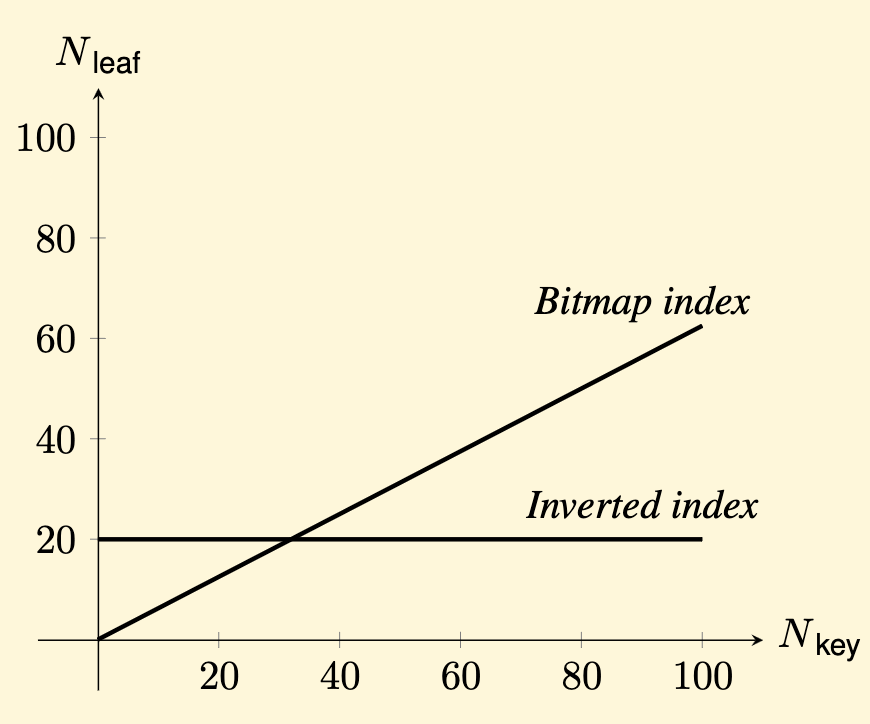
\includegraphics[width=0.5\linewidth]{img/bitmap_vs_inverted.png}
    \caption{Memory usage of bitmap and inverted indexes.}
    \label{fig:bitmap-vs-inverted}
\end{figure}

\subsection{Multidimensional Data Organization}

Multidimensional (or spatial) data is used to represent geometric objects and their position in a multidimensional space. Each record represents a point in the space, has a certain number of attributes that each represent the coordinates. Some common queries in multidimensional datasets are searching for points that fall within a specified rectangular area, and searching for a point's nearest neighbor(s). A typical organization with a B$^+$-tree may not be a good solution, since it does not capture ``closeness'' among points on more than one attribute at a time (the one chosen as key).

A way to solve this issue is to partition the space into areas with the same amount of points, so that each partition can be mapped to a separate page and allow quick retrieval of points that are spatially close together. Consider the dataset represented in Figure \ref{fig:multidim-start}, and suppose that pages have a capacity of 2. The data space is first divided choosing a division value $d$ on one coordinate, so that all points whose attribute value for that coordinate is less than $d$ are inserted into a page, those with a higher value are inserted into the other one. $d$ is usually chosen as the half of the range or the median value. The first split is in Figure \ref{fig:multidim-index} (a), done on the $x$ axis. If the partitions are still too big to fit into pages, then a split is repeated considering another axis (Figure \ref{fig:multidim-index} (b)). The splits continue alternating axes until each partition contains a small enough number of records. All the records belonging to the same partition will be found in the same page.

\begin{figure}[ht]
\centering
\begin{minipage}{0.49\textwidth}
    \centering
    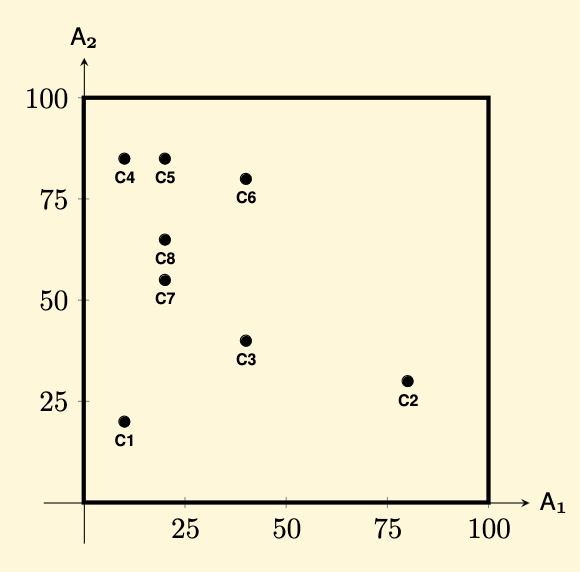
\includegraphics[width=0.5\linewidth]{img/multidim_start.png}
    \caption{Graphical representation of a two-dimensional dataset.}
    \label{fig:multidim-start}
\end{minipage}
\hfill
\begin{minipage}{0.49\textwidth}
    \centering
    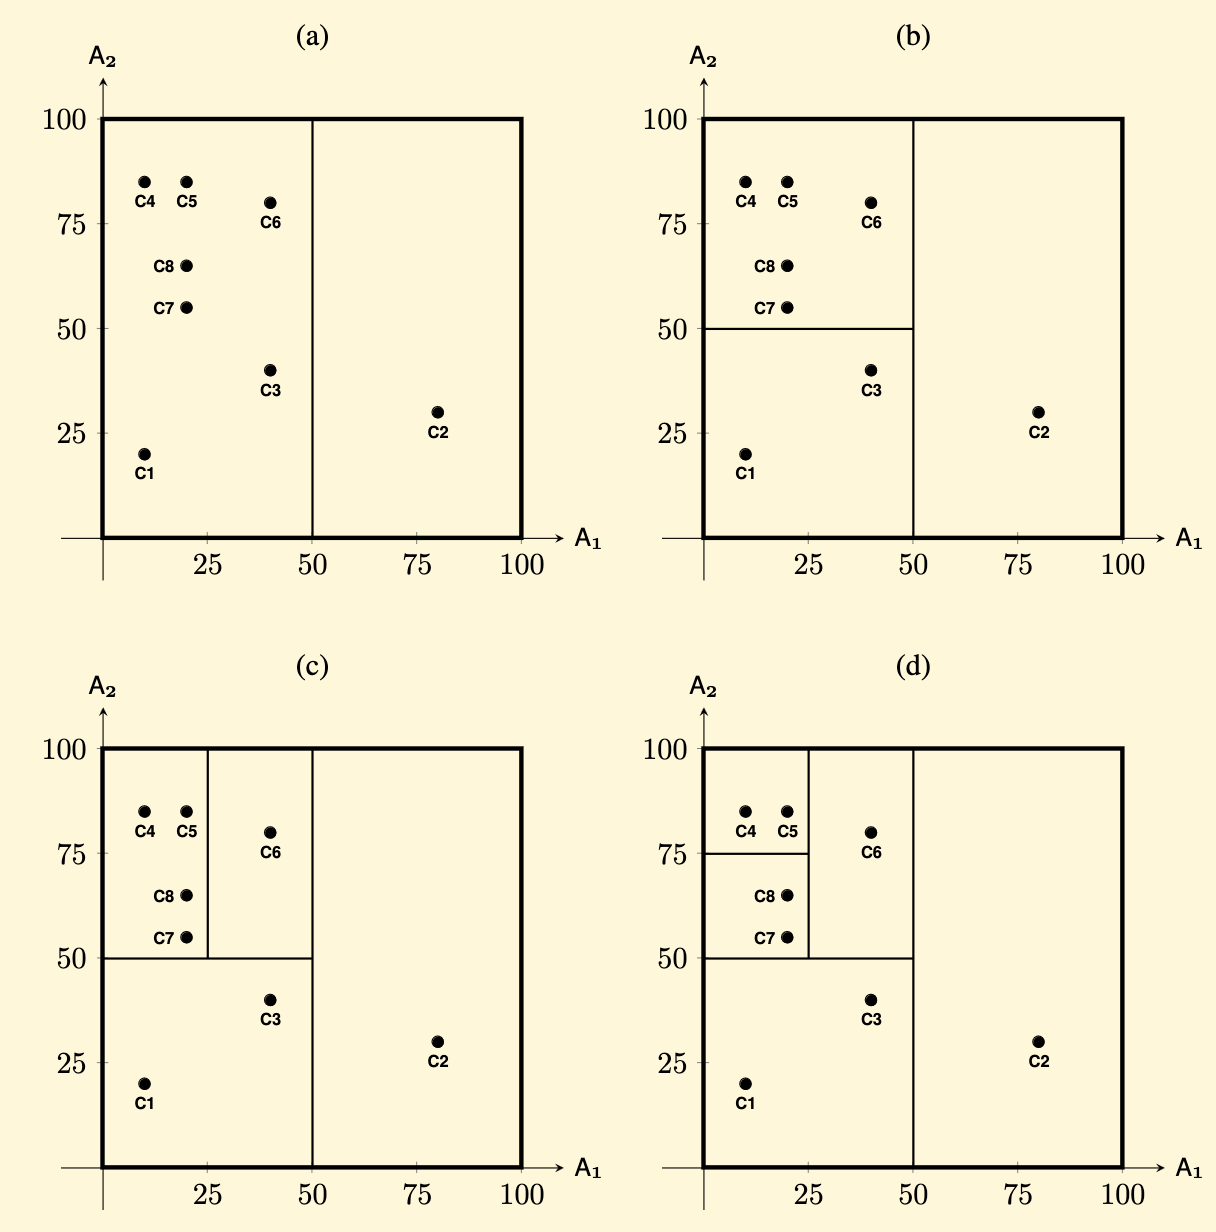
\includegraphics[width=\linewidth]{img/multidim_index.png}
    \caption{Division of the space into partitions.}
    \label{fig:multidim-index}
\end{minipage}
\end{figure}

\subsubsection{G-trees}

G-trees are the data structure used to store multidimensional indexes, where each partition is identified by a \textbf{partition code}. As the space is partitioned, a sort of ``decision tree'' is built, where each node corresponds to an attribute test condition, alternating the attributes at each level. Partition codes are assigned as follows:
\begin{itemize}
    \item The initial, intact, region is identified by the empty string;

    \item After the first split, the two partitions produced are identified with the strings ``0'' and ``1';

    \item When each partition of the previous step is split along the other axis, the new partitions will be ``00'' and ``01'', and ``10'' and ``11'', and so on.

    \item In general, when a partition $R$ is split, the subpartitions will have a code that is equal to the code of the parent and 0/1 appended at the end.
\end{itemize}
Each partition code is then padded so that they all reach $M$ bits, where $M$ is the maximum number of splits made. The G-tree stores these codes like a B$^+$-tree, where the leaves contain all the codes and the internal nodes alternate pointers to leaves and duplicate keys.
\begin{figure}[ht]
    \centering
    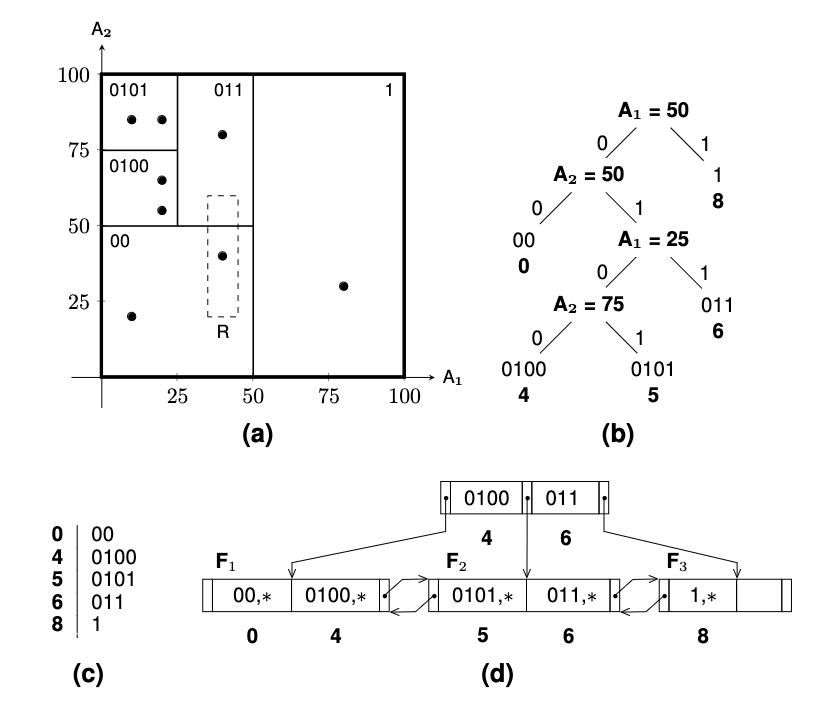
\includegraphics[width=0.5\linewidth]{img/G-tree.png}
    \caption{Example of partition coding.}
    \label{fig:G-tree}
\end{figure}
After the tree has been constructed, point search, insertion, deletion, and spatial range search can be done efficiently. To search a point $P$ with coordinates $(x, y)$, the partition code of the point is retrieved (if it is present), and the code is then used to search in the G-tree.

Range search is done by specifying a range for each axis. The search starts by identifying the lower left and upper right vertices of the rectangle area; the G-tree is searched for the nodes that contain these vertices, and for each leaf between them, the elements are searched, selecting all leaves that directly intersect with the search region.

For point insertion, first the G-tree is searched to find the partition that should contain the point; then, if that partition/leaf is not full, the point is simply inserted, otherwise, the partition must be split into two. Each partition is associated with the correct partition code, and if needed (the split adds a new level to the split tree) all other codes' padding is adjusted. The points in the original partition are distributed between the pages referred by the two leaves accordingly, and the parent node is updated with the new pointer and the duplicate key. If an overflow happens in the parent node, the same procedure seen for B$^+$-trees happens.

To delete a point, it is first searched in the G-tree, and the record is deleted. If the partition becomes empty, its code is removed from the tree. If the partition is the result of a split, and it can be merged with its sibling, then the merge is done and the two partition codes are replaced by the partition code of their parent.
\chapter{Access Method Management}

The Access Methods Manager provides an interface with several operations to interact with the organizations and indexes implemented by the Storage Structure Manager, so that data can be transferred between main and permanent memory. The language used to implement these operations transform the machine into an \textbf{abstract database machine}, called the database management system. Abstract database machines are divided into two parts:
\begin{itemize}
    \item \textbf{Relational Engine}, or abstract machine for the logical data model. Includes modules to support the execution of SQL commands;
    \item \textbf{Storage Engine}, or abstract machine for physical data model. Includes modules to execute operations on the data in permanent memory.
\end{itemize}

\section{Storage Engine}

The interface of the Storage Engine depends on the data structures used in permanent memory. Normally, it is not directly available to the user, who will instead interact with the Relational Engine which in turn will communicate with the Storage Engine. We will consider an interface inspired by that of the relational system JRS, which stores relations into heap files and provides B$^+$-tree indexes.

\paragraph{Data and Transactions}

\begin{itemize}
    \item $beginTransaction : null \mapsto TransactionId$
    
    \item $commit : TransactionId \mapsto null$
    
    \item $abort : TransactionId \mapsto null$
    
    \item $createDB : Path \times DBName \times TransactionId \mapsto DB$
    
    \item $createHF : DB \times Path \times HFName \times TransactionId \mapsto HF$
    
    \item $createIdx : DB \times Path \times IdxName \times HFName \times Attr \times Ord \times Unique \times TransactionId \mapsto Idx$
    
    \item $dropBD : DBName \times TransactionId \mapsto null$
    
    \item $dropHF : HFName \times TransactionId \mapsto null$
    
    \item $dropIdx : IdxName \times TransactionId \mapsto null$
\end{itemize}

\paragraph{Heap File}

\begin{itemize}
    \item $HFopen : DB \times HFName \times TransactionId \mapsto HF$

    \item $HFCcose: HF \mapsto null$

    \item $HFgetRecord : HF \times RID \mapsto Record$

    \item $HFdeleteRecord : HF \times RID \mapsto null$

    \item $HFupdateRecord : HF \times RID \times FieldNum \times NewField \mapsto null$

    \item $HFinsertRecord : HF \times Record \mapsto RID$

    \item $HFgetNPage : HF \mapsto int$

    \item $HFgetNRec : HF \mapsto int$
\end{itemize}

\paragraph{Indexes}

\begin{itemize}
    \item $Iopen : DB \times IdxName \times TransactionId \mapsto Idx$

    \item $Iclose : Idx \mapsto null$

    \item $IdeleteEntry : Idx \times Entry \mapsto null$ ($Entry = Value \times RID$)

    \item $IinsertEntry : Idx \times Entry \mapsto null$
    
    \item $IgetNKey : Idx \mapsto int$
    
    \item $IgetNLeaf : Idx \mapsto int$

    \item $IgetMin : Idx \mapsto Value$

    \item $IgetMax : Idx \mapsto Value$
\end{itemize}

\section{Access Method Operators}

The following operations transfer data between main and permanent memory. Records of a heap file or of an index are accessed by scans: a heap file scan operator reads each record one after the other, while an index scan operator provides a way to efficiently retrieve the RID of the records. Heap file and index scan operators are implemented using a \textbf{cursor} (or \textbf{iterator}), which is an object with methods that can return one record at a time and move across records. The typical structure of program that scans heap files/indexes is:
\begin{algorithm}
\caption{Typical structure of program that uses scan operators.}
\begin{algorithmic}[1]
    \While{$! C.isDone()$}
        \State $Val = C.getCurrent()$
        \State $\dots$
        \State $C.next()$
    \EndWhile
\end{algorithmic}
\end{algorithm}
Here $C$ is the cursor object.

\paragraph{Heap File Scan}

\begin{itemize}
    \item $HFSopen : HF \mapsto HFS$

    \item $HFSisDone : HFS \mapsto bool$

    \item $HFSgetCurrent : HFS \mapsto RID$

    \item $HFSnext : HFS \mapsto null$

    \item $HFSreset : HFS \mapsto null$

    \item $HFSclose : HFS \mapsto null$
\end{itemize}

\paragraph{Index Scan}

\begin{itemize}
    \item $ISopen : Idx \times fstKey \times lstKey \mapsto IS$

    \item $ISisDone : IS \mapsto bool$

    \item $ISgetCurrent : IS \mapsto null$

    \item $ISreset : IS \mapsto null$

    \item $ISclose : IS \mapsto null$
\end{itemize}

\section{Physical Plans}

When a SQL query must be executed, it is first represented as a \textbf{logical plan}, which is a tree representation of the query, and is eventually transformed in a form that can be more efficiently evaluated. This transformed logical plan is then translated into a \textbf{physical plan}, which contains as nodes the actual physical operators that can implement that query. Each operator in a plan is an iterator that uses a ``pull'' interface: when an operator receives a request from above, it ``pulls'' on its input node(s) and computes the result, returning it to its parent operator. An operator interface provides the necessary methods \textit{open}, \textit{next}, \textit{isDone}, and \textit{close}, implemented using the Storage Engine interface.
\chapter{Physical Relational Operators}

One of the most important components in a DBMS is the \textbf{Query Manager}, which is responsible for scheduling queries and directing them to the correct tables. Part of the Query Manager is the \textbf{Query Optimizer}, which has the task of determining how to execute a query in the most efficient way possible, considering the physical parameters involved, the data organization, and the presence or absence of indexes.

This chapter will deal with how different physical operators are implemented, for the following operations:
\begin{itemize}
    \item Projection;
    \item Selection;
    \item Grouping;
    \item Set operations;
    \item Join.
\end{itemize}
Then, it will discuss how the optimizer uses these operators to generate efficient physical plans. In general, the problem will be studied under certain assumptions, illustrated in the next sections.

\section{Selectivity Factors}

The selectivity factor of a condition is an estimate of the percentage of the records in a relation which satisfy that condition. The simplest way to estimate this percentage is by assuming the data is uniformly distributed. The selectivity factor of different conditions in reported in table \ref{tab:sf-cond}. The last column is a constant value that is used if not enough information is known to calculate the actual $sf$, or when the attribute is non-numeric. 
\begin{table}[h]
\centering
\SetTblrInner{rowsep=5pt}
    \begin{tblr}{
        hlines,
        vlines,
        columns={145pt, c, m},
        column{1}={80pt}
    }
        Condition & Calculated $sf$ & Approx. $sf$ \\
    \hline
        $A = v$ & $\dfrac{1}{N_{key}}$ & $\dfrac{1}{10}$ \\
        $A > v$ & $\dfrac{\max(A) - v}{\max(A) - \min(A)}$ & $\dfrac{1}{3}$ \\
        $A < v$ & $\dfrac{v - \min(A)}{\max(A) - \min(A)}$ & $\dfrac{1}{3}$ \\
        $v_1 < A < v_2$ & $\dfrac{v_2 - v_1}{\max(A) - \min(A)}$ & $\dfrac{1}{4}$ \\
        $A_1 = A_2$ & $\dfrac{1}{\max(N_{key}(A), N_{key}(B))}$ & $\dfrac{1}{10}$ \\
        $\psi_1 \land \psi_2$ & $sf(\psi_1) \times sf(\psi_2)$ & - \\
        $\psi_1 \lor \psi_2$ & $sf(\psi_1) + sf(\psi_2) -$ $sf(\psi_1) \times sf(\psi_2)$ & - \\
    \end{tblr}
    \caption{Selectivity factors of different conditions.}
    \label{tab:sf-cond}
\end{table}

In many cases, however, attribute values follow non-uniform distributions, making these estimates wrong. The selectivity factor of a condition can be better approximated by knowing the actual distribution of the data, but storing the information needed to have full knowledge about it would occupy too much space. The solution preferred by DBMSs is to use a histogram with binned ranges of values in order to approximate the actual distribution.

There are two types of histograms: \textbf{equi-width} and \textbf{equi-height}. Equi-width histograms are obtained by binning values so that each bin has the same amount of elements $n$. For each bin, the sum of the counts of all elements inside that bin is stored. To find the selectivity factor for an equality search given a value $v$, it will be given by the sum associated with the bin $v$ belongs to, divided by $n$. For inequality/range searches, the selectivity factor will consider the sum associated with all the bins completely included in the range, plus the term that is given by the bin(s) corresponding to the extreme(s) of the condition.

The problem with equi-width histograms is that while they provide better approximations than a blind uniform distribution assumption, they are not able to correctly approximate the distribution of data to a sufficiently high precision. This is why equi-height histograms are used instead. These histograms are divided into bins such that the sum of counts of values within each (their ``height'') is equal across all of them. To store this type of histogram, the only information needed is the number of elements in each bin.

\begin{figure}[h]
    \centering
    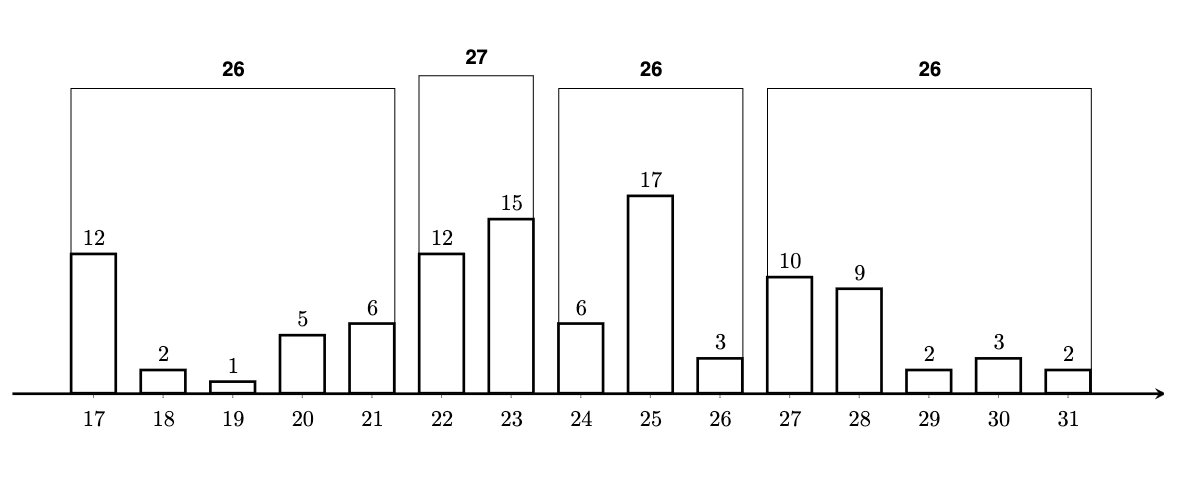
\includegraphics[width=0.7\linewidth]{img/equiheight.png}
    \caption{An equi-height histogram.}
    \label{fig:equi-height}
\end{figure}

Still, the approximation done by these histograms may not be accurate if the distribution within a bin is not uniform. For example, in Image \ref{fig:equi-height}, the third bin has follows a Gaussian distribution. If a query requests all records whose values for that attribute is equal to 24, the selectivity factor approximation will be much higher than the real one; if a query instead requests records with value 25, the approximation will be much lower.

\section{Physical Operators}

\subsection{Operators for Relation}

\paragraph{TableScan($R$)}
Returns all the records in $R$, in the same order as they are stores. It costs
\begin{equation*}
    C = N_{pag}(R)
\end{equation*}
The result size is
\begin{equation*}
    E_{rec} = N_{rec}(R)
\end{equation*}

\paragraph{SortScan($R, \{A_i\}$)}
Returns all the records in $R$ sorted in ascending order on the attribute $A_i$. Sorting is done with a merge sort algorithm. It costs
\begin{equation*}
    C = \begin{cases}
        N_{pag}(R) & N_{pag}(R) < B \\
        3 \times N_{pag}(R) & N_{pag}(R) \leq B \times (B-1) \\
        N_{pag}(R) + 2 \times N_{pag}(R) \times \ceil{log_{B-1}(N_{pag}(R) / B)} & \text{else}
    \end{cases}
\end{equation*}
The result size is
\begin{equation*}
    E_{rec} = N_{rec}(R)
\end{equation*}

\paragraph{IndexScan($R, I$)}
Returns the records of $R$ sorted by the attribute the index $I$ is defined on. It costs
\begin{equation*}
    C = \begin{cases}
        N_{leaf}(I) + N_{pag}(R) & \text{if $I$ is clustered} \\
        N_{leaf}(I) + N_{rec}(R) & \text{if $I$ is on a key of $R$} \\
        N_{leaf}(I) + \ceil{N_{key}(I) \times \phi(\ceil{N_{rec}(R) / N_{key}(I)}, N_{pag}(R))} & \text{else}
    \end{cases}
\end{equation*}
The result size is
\begin{equation*}
    E_{rec} = N_{rec}(R)
\end{equation*}

\paragraph{IndexSequentialScan($R, I$)}
Returns the records of $R$, stored with the primary organization index sequential file $I$, sorted in ascending order on the primary key values. It costs
\begin{equation}
    C = N_{leaf}(I)
\end{equation}
The result size is
\begin{equation*}
    E_{rec} = N_{rec}(R)
\end{equation*}

\subsection{Operators for Projection}

\paragraph{Project($O, \{A_i\}$)}
Projects the records of $O$ over the attributes $\{A_i\}$. It costs
\begin{equation*}
    C = C(O)
\end{equation*}
The result size is
\begin{equation*}
    E_{rec} = E_{rec}(O)
\end{equation*}

\paragraph{IndexOnlyScan($R, I, \{A_i\}$)}
Returns the sorted records of $R$, projecting them over the attributes $\{A_i\}$ on which the index $I$ is on (or contains them as prefix). It costs
\begin{equation*}
    C = N_{leaf}(I)
\end{equation*}
If a tuple of values for the attributes $\{A_i\}$ is associated with $n$ different RIDs, it is returned $n$ times. The result will not contain duplicates if the attributes are relation keys (they uniquely identify records). The result size is
\begin{equation*}
    E_{rec} = N_{rec}(R)
\end{equation*}

\subsection{Operators for Duplicate Elimination}

\paragraph{Distinct($O$)}
Returns the records of $O$ eliminating all duplicates. This operator requires that the records of $O$ are \textbf{grouped} (if $r_i = r_j$, and $i < l < j$, then $r_i = r_l = r_j$). When a collection of records is sorted, it is also grouped. It costs
\begin{equation*}
    C = C(O)
\end{equation*}
If there's only one attribute in $O$, then the result size is
\begin{equation*}
    E_{rec} = N_{key}(A)
\end{equation*}
If instead it contains multiple attributes, the result size is
\begin{equation*}
    E_{rec} = \min(|O|/2, \prod_i N_{key}(A_i))
\end{equation*}
This is a pessimistic estimate: it assumes that there is a record for each set of values taken from the attributes in $O$, but this is often not the actual result. For example, imagine a database containing data about students enrolled at a university, and the two attributes represent their first name and last name respectively: it is unrealistic to expect that there will be a different student for each first name-last name combination, even if the two attributes are loosely correlated.

\paragraph{HashDistinct($O$)}
Returns the records of $O$ without duplicates using and hash technique. This technique has two phases: \textbf{partitioning} and \textbf{duplicate elimination}. Assume the query processor has $B+1$ buffer pages. In the partitioning phase, for each record in $O$ the hash function $h_1$ is applied, distributing records uniformly across the $B$ pages. Once a page $i$ is full, it is written to the $T_i$ partition file. At the end of the phase, all records will be scattered across $B$ files, each of which contains records with the same hash value; this means that duplicates are found in the same partition.

In the duplicate elimination phase, the process becomes an intra-partition problem. Each $T_i$ file is read page-by-page, eliminating duplicates using the hash function $h_2$. A record is deleted when it collides with another record with the same hash value according to $h_2$ and the two records are identical. Assuming each partition occupies at most $B$ pages, at the end of the partition, the $B$ pages are cleared, and the duplicate elimination is applied to the records in the next partition. If the number of pages is greater than $B$, then a hash-based projection technique is applied recursively by dividing the partition into subpartitions. This degrades performances. The operator costs:
\begin{equation*}
    C = C(O) + 2 \times N_{pag}(O)
\end{equation*}
The result size is the same as Distinct, so
\begin{equation*}
    E_{rec} = N_{key}(A)
\end{equation*}
if there's only one attribute in $O$, and
\begin{equation*}
    E_{rec} = \min(|O|/2, \prod_i N_{key}(A_i))
\end{equation*}
if $O$ contains multiple attributes.

\subsection{Operators for Sort}

\paragraph{Sort($O, \{A_i\}$)}
Returns the records of $O$ sorted on the attributes $\{A_i\}$. The sorting algorithm used is merge-sort, so its cost is
\begin{equation*}
    C = \begin{cases}
        C(O) & N_{pag}(O) < B \\
        C(O) + 2 \times N_{pag}(O) & N_{pag}(O) \leq B \times (B-1) \\
        C(O) + 2 \times N_{pag}(O) \times \ceil{log_{B-1}(N_{pag}(O) / B)} & \text{else}
    \end{cases}
\end{equation*}
The result size is
\begin{equation*}
    E_{rec} = N_{rec}(O)
\end{equation*}

\subsection{Operators for Selection}

\paragraph{Filter($O,\psi$)}
Returns the records of $O$ that satisfy the condition $\psi$. It costs
\begin{equation*}
    C = C(O)
\end{equation*}
The result size is
\begin{equation*}
    \ceil{sf(\psi) \times N_{rec}(O)}
\end{equation*}

\paragraph{IndexFilter($R,I,\psi$)}
Returns the records of $R$ that satisfy the condition $\psi$ using the index $I$, defined on the attributes involved in $\psi$, sorted according to $I$. The condition is a predicate or a conjunction of predicates that only involve the attributes found in the prefix of the index search key.

IndexFilter always appears as a leaf node in a physical plan. This operator uses the index to find the sorted set of RIDs of all records that satisfy the condition, then it retrieves the records from disk. The cost can be broken down as
\begin{equation*}
    C = C_I + C_D
\end{equation*}
\begin{itemize}
    \item If the index is clustered:
    \begin{align*}
        &C_I = \ceil{sf(\psi) \times N_{leaf}(I)} \\
        &C_D = \ceil{sf(\psi) \times N_{pag}(R)}
    \end{align*}

    \item If the index is unclustered:
    \begin{align*}
        &C_I = \ceil{sf(\psi) \times N_{leaf}(I)} \\
        &C_D = \ceil{sf(\psi) \times N_{key}(I)} \times \ceil{\Phi(\ceil{N_{rec}(R) / N_{key}(I)}, N_{pag}(R))}
    \end{align*}
    If the index is defined on a key of $R$, then
    \begin{equation*}
        C_D = \ceil{sf(\psi) \times N_{rec}(R)}
    \end{equation*}
\end{itemize}
The result size is
\begin{equation*}
    E_{rec} = \ceil{sf(\psi) \times N_{rec}(R)}
\end{equation*}

\paragraph{IndexSequentialFilter($R,I,\psi$)}
Returns the sorted records of $R$, stored with the primary organization index sequential file $I$, satisfying the condition $\psi$, which involves only the attributes of the index search key. It costs
\begin{equation*}
    C = \ceil{sf(\psi) \times N_{leaf}(I)}
\end{equation*}
The result size is
\begin{equation*}
    E_{rec} = \ceil{sf(\psi) \times N_{rec}(R)}
\end{equation*}

\paragraph{IndexOnlyFilter($R, I, \{A_i\}, \psi$)}
Returns the sorted records of the projection on $R$ returning only the values for $\{A_i\}$ that satisfy $\psi$, using only the index $I$. It costs
\begin{equation*}
    C = \ceil{sf(\psi) \times N_{leaf}(I)}
\end{equation*}
The result size is
\begin{equation*}
    E_{rec} = \ceil{sf(\psi) \times N_{rec}(R)}
\end{equation*}

\subsection{Operators for Grouping}

\paragraph{GroupBy($O, \{A_i\}, \{f_i\}$)}
Returns the records of $O$ sorted on $\{A_i\}$, applying the aggregation functions $\{f_i\}$. The records in $O$ must already be sorted beforehand. It costs
\begin{equation*}
    C = C(O)
\end{equation*}

\paragraph{HashGroupBy($O, \{A_i\}, \{f_i\}$)}
Returns the records of $O$ grouped by $\{A_i\}$, applying the aggregation functions $\{f_i\}$. The records are not sorted on $\{A_i\}$. The grouping is done using two phases, like HashDistinct. In the first phase, called partitioning phase, a partition is created using the hash function $h_1$; in the second phase, called grouping, the records of each partition are grouped using the hash function $h_2$ applied to all grouping attributes. When two records with the same grouping attributes are found, a step to compute the aggregate function is applied. The operator costs
\begin{equation*}
    C = C(O) + 2 \times N_{pag}(O)
\end{equation*}

For both the previous two operators, the result size is calculated as for the duplicate elimination. If there's only one attribute in $O$, then the result size is
\begin{equation*}
    E_{rec} = N_{key}(A)
\end{equation*}
If instead it contains multiple attributes, the result size is
\begin{equation*}
    E_{rec} = \min(|O|/2, \prod_i N_{key}(A_i))
\end{equation*}

\subsection{Operators for Join}

\paragraph{NestedLoop($O_E, O_I, \psi_J$)}
Joins the external operand $O_E$ with the internal operand $O_I$ with the following algorithm:
\begin{algorithm}
\begin{algorithmic}
    \For{$r \in O_E$}
        \For{$s \in O_I$}
            \State If $\psi_J$, add $<r,s>$ to the result.
        \EndFor
    \EndFor
\end{algorithmic}
\end{algorithm} \\
It costs
\begin{equation*}
    C = C(O_E) + E_{rec}(O_E) \times C(O_I)
\end{equation*}
The result size is
\begin{equation*}
    E_{rec} = sf(\psi_j) \times E_{rec}(O_E) \times E_{rec}(O_I)
\end{equation*}

\paragraph{PageNestedLoop($O_E, O_I, \psi_J$)}
Joins the external operand with the internal operand by scanning $O_I$ once per page of $O_E$ (and not once per record, as for NestedLoop). The algorithm used is the following:
\begin{algorithm}
\begin{algorithmic}
    \For{$p_r$ of $O_E$}
        \For{$p_s$ of $O_I$}
            \For{$r \in p_r$}
                \For{$s \in p_s$}
                    \State If $\psi_J$, add $<r,s>$ to the result. 
                \EndFor
            \EndFor
        \EndFor
    \EndFor
\end{algorithmic}
\end{algorithm} \\
The cost of the operator is
\begin{equation*}
    C = C(O_E) + N_{pag}(O_E) \times C(O_I)
\end{equation*}
The algorithm cost is lower when the external operand is the one with fewer pages.
The result size is
\begin{equation*}
    E_{rec} = sf(\psi_j) \times E_{rec}(O_E) \times E_{rec}(O_I)
\end{equation*}

\paragraph{BlockNestedLoop($O_E, O_I, \psi_J$)}
Joins the external operand $O_E$ with the internal operand $O_I$ by extending PageNestedLoop using more memory for a group of pages of the external operand. Assume the operands are TableScan of tables $R$ and $S$, and that the query processor has $B+2$ pages in the buffer. $B$ pages are used for the external operand, 1 page for an input page of $S$, and 1 page is reserved as the output buffer. For each record $r$ of a page group of $R$, and for each joining record $s$ of a page in $S$, $<r,s>$ is written to the output buffer page.

The cost of the operator is
\begin{equation*}
    C = N_{pag}(R) + \ceil{N_{pag}(R)/B} \times N_{pag}(S)
\end{equation*}
The cost is lower if the external relation has fewer pages than the internal one. If the $B$ pages are enough to contain one of the two relations, then the cost is reduced to
\begin{equation*}
    N_{pag}(R) + N_{pag}(S)
\end{equation*}
The result size is
\begin{equation*}
    E_{rec} = sf(\psi_j) \times E_{rec}(O_E) \times E_{rec}(O_I)
\end{equation*}
This operator is not convenient to use when the operators require too many pages (i.e., $N_{pag}R \geq B^2$).

\paragraph{IndexNestedLoop($O_E, O_I, \psi_J$)}
This operator requires that there is an index on the join column of the internal operand, and performs a join with the following algorithm:
\begin{algorithm}
\begin{algorithmic}
    \For{$r \in O_E$}
        \For{$s \in$ IndexFilter($O_I, I, O_E.e1 = O_I.i1$)}
            \State Add $<r,s>$ to the result.
        \EndFor
    \EndFor
\end{algorithmic}
\end{algorithm} \\
It costs
\begin{equation*}
    C = C(O_E) + E_{rec}(O_E) \times (C_I + C_D)
\end{equation*}
where $C_I$ and $C_D$ are the costs to retrieve the relevant index records and the data from disk. If the internal operand is an IndexFilter($S,I,\psi_J$), the result size is
\begin{equation*}
    E_{rec} = \ceil{sf(\psi_J) \times E_{rec}(O_E) \times N_{rec}(S)}
\end{equation*}
if instead it is a Filter(IndexFilter($S, I, \psi_J$), $\psi$), the result size is
\begin{equation*}
    E_{rec} = \ceil{sf(\psi_J) \times E_{rec}(O_E) \times (sf(\psi) \times N_{rec}(S))}
\end{equation*}

\paragraph{MergeJoin($O_E, O_I, \psi_J$)}
This operator requires that $O_E$ and $O_I$ are sorted on the same join attributes, and that in the join condition, $O_E.A_i$ is a key of $O_E$. Since this join attribute has distinct values in $O_E$, the algorithm reads the records of $O_E$ one by one, and reads all records of $O_I$ with the same values (which will be found one after the other). This operator costs
\begin{equation*}
    C = C(O_E) + C(O_I)
\end{equation*}
The result size is
\begin{equation*}
    E_{rec} = \ceil{sf(\psi_J) \times E_{rec}(O_E) \times E_{rec}(O_I)}
\end{equation*}

\paragraph{HashJoin($O_E, O_I, \psi_J$)}
Returns the join result with a hash technique in two phases. In the first phase, called partitioning phase, the records of both operands are partitioned using the hash function $h_1$, similarly to HashDistinct. In the second phase, called \textbf{probing} (or \textbf{matching}), for each $B_i$ partition, the records of $O_E$ are read and inserted into the buffer hash table with $B$ pages using the hash function $h_2$. The records of $O_I$ are read one page at a time, $h_2$ is applied to them, and if there is a match with the records in $O_E$, the joined record is added to the result.

Assuming $N_{pag}(O_E)/B < B$ and that the pages are uniform, the cost of the operator is
\begin{equation*}
    C = C(O_E) + C(O_I) + 2 \times (N_{pag}(O_E) + N_{pag}(O_I))
\end{equation*}
where $(C(O_E) + C(O_I) + (N_{pag}(O_E) + N_{pag}(O_I))$ is the cost of the partitioning phase, and $(N_{pag}(O_E) + N_{pag}(O_I))$ is the cost of the probing phase. However, if the pages are not uniform, the resulting partitions will not have the same size, they may not fit in $B$. The cost can be generalized to
\begin{equation*}
    C = (\log_B(N_{pag}(O_E)) \times 2 - 2) \times (N_{pag}(O_E) + N_{pag}(O_I))
\end{equation*}
If $N_{pag}(O_E) < B$, the cost is 0.

The result size is
\begin{equation*}
    E_{rec} = \ceil{sf(\psi_J) \times E_{rec}(O_E) \times E_{rec}(O_I)}
\end{equation*}
\chapter{Query Optimization}

The optimizer is a key component of the Query Manager. Its role is to select the optimal physical plan to execute queries using the operators and data structures provided by the Storage Engine. This chapter will show how functional dependencies are used for not only relational schema design, but also for optimization.

\section{Query Processing and Execution}

In general, there are many strategies to execute a query, in particular when it is complex. The problem of optimizing a query is influenced by the fact that a query can be written in several equivalent ways, and relational algebra operators can be implemented using different physical operators.

Query processing is divided into four stages:
\begin{itemize}
    \item \textbf{Query analysis}, in which the correctness of the SQL query is checked, and the query is translated into its internal form, typically based on relational algebra;

    \item \textbf{Query transformation}, in which the logical plan is transformed into an equivalent one that provides a better query performance;

    \item \textbf{Physical plan generation}, in which alternative physical plans are generated and evaluated, of which the one with the lowest cost is chosen;

    \item \textbf{Query evaluation}, in which the chosen physical plan is executed.
\end{itemize}
Query transformation and Physical plan generation are often considered part of the same phase, and are called Query optimizer.

The most interesting transformations regard Distinct elimination, GroupBy elimination, Where-subquery elimination, and View elimination.

\section{Functional Dependencies}

\BoxDef{Functional Dependency}{
Given a relation schema $R$ and $X,Y$ subsets of attributes of $R$, a functional dependency $X \rightarrow Y$ (read as ``$X$ determines $Y$'') is a constraint such that, for every possible instance $r$ of $R$ and for any two tuples $t_1, t_2 \in r$:
\begin{equation*}
    t_1[X] = t_2[X] \implies t_1[Y] = t_2[Y] 
\end{equation*}
}
A functional dependency is \textbf{trivial} if the consequent contains attributes also found in the antecedent:
\begin{equation*}
    XY \rightarrow X
\end{equation*}
A functional dependency is \textbf{atomic} if the consequent is composed of only one attribute:
\begin{equation*}
    X \rightarrow A
\end{equation*}
A functional dependency $X \rightarrow A$ is \textbf{canonical} if:
\begin{equation*}
    X \rightarrow A
\end{equation*}
holds true, but
\begin{equation*}
    X' \rightarrow A, \ \forall X' \subset X
\end{equation*}
does not. Every non-trivial dependency also contains one or more canonical dependencies, obtained by removing extraneous attributes. \\
A \textbf{key} is a set of attributes $K$ such that:
\begin{equation*}
    K \rightarrow T
\end{equation*}
holds and is canonical. \\
The \textbf{union rule} states that:
\begin{equation*}
    X \rightarrow A_1 \dots A_n \iff X \rightarrow A_1, \dots, X \rightarrow A_n
\end{equation*}
To specify that an attribute has a constant value for all tuples, the rule used is:
\begin{equation*}
    \emptyset \rightarrow Y
\end{equation*}

\BoxDef{Logical Implication}{
Given a set of functional dependencies $F$ on a relation schema $R$, a functional dependency $X \rightarrow Y$ is derived (implied) from $F$ if every instance of $R$ that satisfies $F$ also satisfies $X \rightarrow Y$:
\begin{equation*}
    F  \vdash X \rightarrow Y
\end{equation*}
This property holds if $X \rightarrow Y$ can be derived from $F$ using any of \textbf{Armstrong's axioms}:
\begin{itemize}
    \item $Y \subseteq X \implies X \rightarrow Y$ (Reflexivity)
    \item $X \rightarrow Y, Z \subseteq T \implies XZ \rightarrow YZ$ (Augmentation)
    \item $X \rightarrow Y, Y \rightarrow Z \implies X \rightarrow Z$ (Transitivity)
\end{itemize}
}
To test whether a functional dependency is implied by a set of functional dependencies, the \textbf{closure} of the antecedent can be calculated.
\BoxDef{Closure of Attribute Set}{
Given a schema $R <T,F>$, and $X \subseteq T$, the closure of $X$ is:
\begin{equation*}
    X^+ = \{A_i \in T | F \vdash X \rightarrow A_i\}
\end{equation*}
}
The following theorem holds true.
\BoxDef{Theorem}{
\begin{equation*}
    F \vdash X \rightarrow Y \iff Y \subseteq X^+
\end{equation*}
}

Consider a query on a set of tables $R_1(T_1), \dots, R_n(T_n)$, such that no attribute name appears in two tables. After joining the tables and performing a Select, assuming the Where condition $C$ is in CNF, these dependencies hold on the final result:
\begin{itemize}
    \item $K_{ij} \rightarrow T_i \ \forall K_{ij}$ key of $T_i$;
    \item $\emptyset \rightarrow A \ \forall A=c$ in $C$;
    \item $A_i \rightarrow A_j$ and $A_j \rightarrow A_i$ $\forall A_i = A_j$.
\end{itemize}

\section{Eliminations}

\subsection{Distinct Elimination}

Distinct normally requires a physical plan with duplicate elimination, and data must be grouped, usually via a sort operation (which is expensive). A query with a Distinct clause is translated into a relational algebra expression with the projection and duplicate elimination operators. To decide whether this duplicate elimination operator is unnecessary, a functional dependency theory algorithm is used. Specifically, the following theorem is used:
\BoxDef{Theorem}{
Let $A$ be the set of attributes of the result and $K$ the union of the attributes of the key for every table used in the query. If $A \rightarrow K$, then the duplicate elimination is unnecessary.
}
To find out whether $A \rightarrow K$, the closure of $A$ is computed.

If the query contains a GroupBy clause, then the theorem holds for $G$ (the grouping attributes) instead of $K$.

\subsection{GroupBy Elimination}

GroupBy also usually requires a sort operation. A GroupBy can be eliminated if either each group only has one record, or if there is only one group. The first case can be tested for as seen for Distinct, since it's equivalent to checking if the result contains duplicates. For the second case, we must check that the value of the grouping attributes is the same for each tuple; this is done by verifying that the closure of the empty set ($\{\}^+$) contains all the grouping attributes. 

If aggregation functions are used, Count will be replaced by 1, and Min($A$), Max($A$), Sum($A$), and Avg($A$) will be replaced by $A$.

\subsection{Where-subquery Elimination}

This is one of the most common and important transformations. In general, to execute these queries, the optimizer will generate a physical plan for the subquery, which will be executed for each record processed by the outer query. We will assume all subqueries  have been converted to an equivalent form using Exists, and that no GroupBy appears in the subquery. Given a query in the form
\begin{figure}[H]
    \centering
    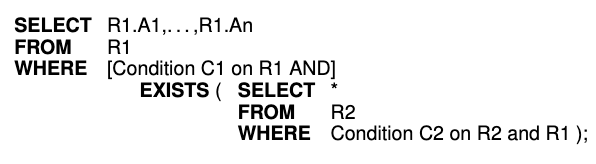
\includegraphics[width=0.75\linewidth]{img/opt_query1.png}   
\end{figure}
\noindent it is equivalent to
\begin{figure}[H]
    \centering
    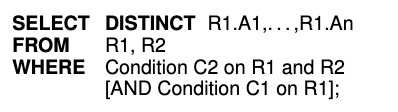
\includegraphics[width=0.5\linewidth]{img/opt_query2.png}
\end{figure}
The Distinct is necessary in the join form when a (1:N) relationship exists between R1 and R2. Note that if only a subset of R1's attributes appears in the Select clause, this transformation will not be correct unless the original query has a Distinct in the outer query.

If the subquery has an aggregation function, then the unnested equivalent requires a GroupBy clause on the projection attributes. A well-known problem is the \textbf{count bug problem}, which arises when the aggregation function is Count. In this case, the unnested query join must be replaced by an outer join.
An outer join is represented by a NATURAL RIGHT JOIN, NATURAL LEFT JOIN, or NATURAL FULL JOIN operator; the first one preserves all records from the left operand, the second one preserves all records from the right operand, and the third one preserves all records.

\begin{figure}[h]
\centering
    \begin{minipage}{0.49\textwidth}
    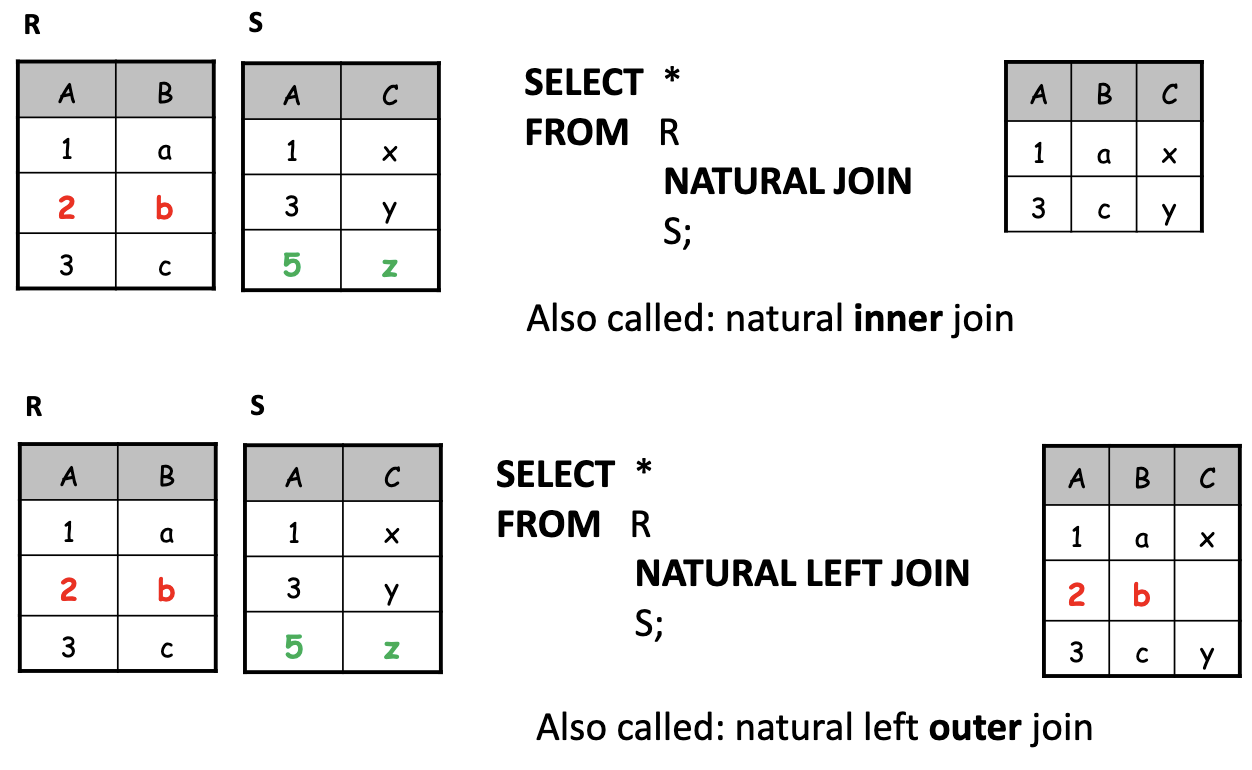
\includegraphics[width=\linewidth]{img/joins1.png}
    \end{minipage} 
    \hfill
    \begin{minipage}{0.49\textwidth}
    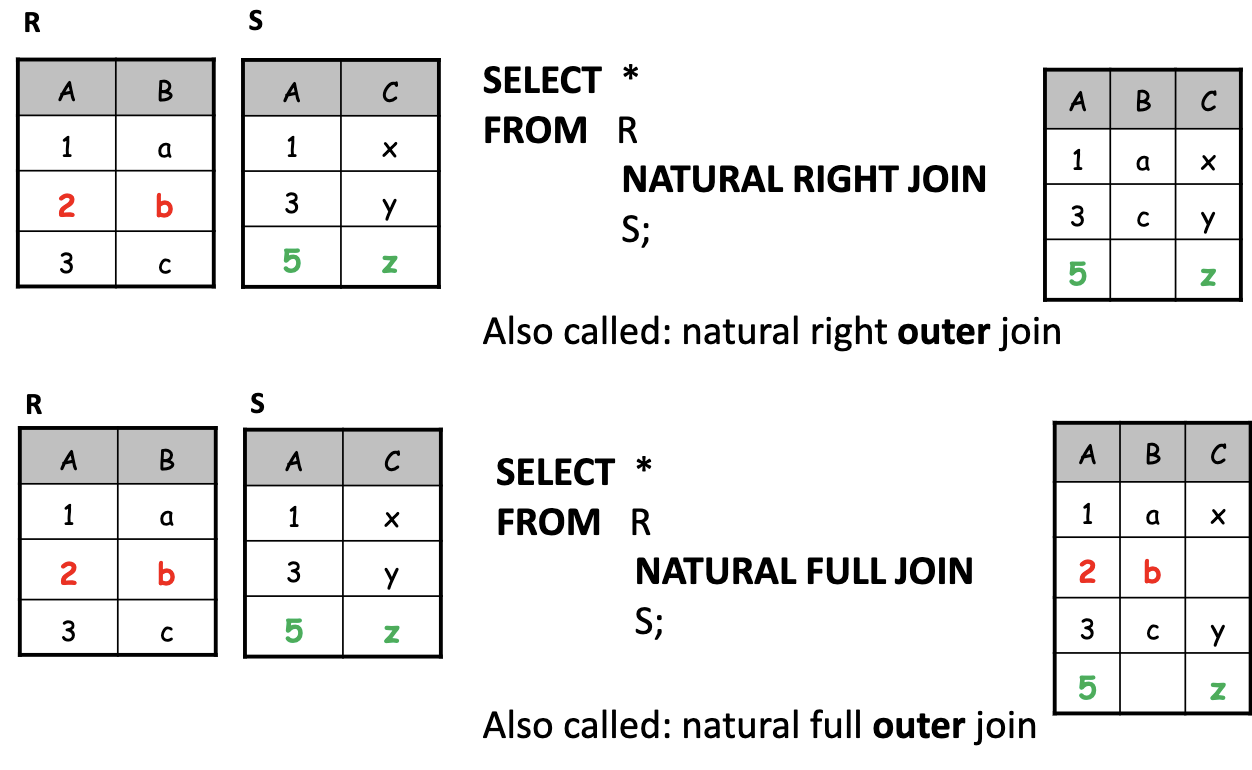
\includegraphics[width=\linewidth]{img/joins2.png}
    \end{minipage}
    \caption{Types of join.}
    \label{fig:joins_in_out}
\end{figure}

\subsection{View Merging}

Complex queries are easier to understand if views are used. The With clause defines temporary views available only to the query in which the clause occurs. When a query generates a view, the optimizer generates a physical sub-plan for the Select that defines the view, and optimizes the query considering the scan as the only operation available for the result of the view; with this technique, the view is optimized separately from the rest of the query.

In the logical plan, the transformation is made by replacing the reference to a view name with the corresponding logical plan. The new logical plan is then rewritten using equivalence rules of relational algebra to put it in the following canonical form:
\begin{equation*}
    \pi^b(\sigma(\gamma(\sigma(^{\bowtie}_J R_i))))
\end{equation*}
The transformation of a query to avoid the use of views defined with a GroupBy generally requires pulling the GroupBy above a join, using the following algebraic equivalence rule:
\begin{equation*}
    ({}_{X_R} \gamma_F(R)) \bowtie_{f_{k} = p_k} S \equiv {}_{X_R \cup A(S)} \gamma_F (R \bowtie_{f_{k} = p_k} S) \,,
\end{equation*}
where $X_R$ is a set of attributes of $R$, $f_k \in X_R$ the foreign key of $R$, and $p_k$ the primary key of $S$ of attributes $A(S)$.

\section{Physical Plan Generation}

With eliminations, a ``random'' physical plan is generated for the query, which is then optimized. Generation, on the other hand, directly finds the best possible physical plan, in two steps: generation of alternative physical query plans, and choice of physical query plan with the lowest estimated cost. To estimate the cost of the entire plan, it is necessary to estimate the cost of the physical operator and the size of the result of every node in the tree (in a bottom-up fashion). The following sections will show how to choose the physical query plan of minimum cost for different types of queries.

\subsection{Single-Relation Queries}

For these queries, the only question to solve is whether to use indexes when accessing the data instead of performing a simple TableScan. Some relations may have single or multiple indexes defined on one or more of their attributes; in that case, the cost of reading the entire table is compared against the cost of reading the index and retrieving the data using the RIDs contained in the index. Usually, using an index is better if the selectivity factor of the query is restrictive enough. A special case happens when the attributes appearing in the Select are included in the prefix of the key of an index of the relation; the query can be evaluated by only reading the index itself, which is much faster than reading the whole table. 

\subsection{Multiple-Relation Queries}

The most important issue in these queries is the order in which the relations are joined. Every permutation of relations yields the same result but corresponds to a different plan; given $n$ relations, there are $n!$ different permutations, each of which generates a huge number of candidates depending on the specific joins performed in the plan. Additionally, there are different choices for the specific physical operator used to implement the join, increasing the total number of possible plans.

The full search in the space of candidates starts by finding which relation is cheaper to access (representing the operator as a standalone plan). Then, the second cheapest plan is chosen among the ones not selected in the previous step and the ones that would be generated by a join of the previously chosen relation with a different one, and so on until the entire query is covered by the physical plan. At each step, the only plans evaluated are the ones behind a so-called ``frontier'', meaning all plans that are direct children of either the (empty) root of the entire search or a plan that has been selected as a minimum cost one.

This algorithm can be incredibly efficient for simpler queries and incredibly slow for complex ones. In the latter case, the algorithm will tend to backtrack to higher levels in the ``tree'' of physical plans explored. A simple pseudocode for this algorithm is presented below.

\begin{algorithm}
\caption{Full search pseudocode.}
\begin{algorithmic}[1]
    \State Initialize $Plans$ to the best plans to access each relation in the query.
    \Loop
        \State Extract the fastest plan $P$ from $Plans$.
        \If{$P$ is complete}
            \State \Return $P$
        \EndIf
        \For{$R$ not in $P$}
            \State Put the best plan between $P \bowtie R$ and $R \bowtie P$ in $Plans$.
        \EndFor
        \State Remove $P$.
    \EndLoop
\end{algorithmic}
\end{algorithm}

Several heuristics have been proposed that can help speed up the algorithm, meaning that the algorithm may not find the optimal physical plan but one that is good enough. The most commonly used heuristics are:
\begin{itemize}
    \item \textbf{Limitation in the number of successors}: each permutation is evaluated by associating the join operators only to the left, creating \textbf{left-deep} trees, where each node from the root up until the second-to-last level has a join as a left child and a relation as a right child (as opposed to \textbf{right-deep} and \textbf{bushy} trees). A left-deep tree has the advantage of allowing the use of an index nested loop join operator. 

    \begin{figure}[h]
        \centering
        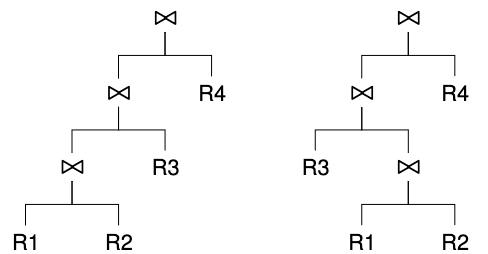
\includegraphics[width=0.5\linewidth]{img/leftdeep_vs_bushy.png}
        \caption{Left-deep tree on the left, bushy tree on the right.}
        \label{fig:ldeep-vs-bushy}
    \end{figure}

    \item \textbf{Greedy search}: once the logical node of minimum cost has been expanded, the other nodes are not considered anymore, avoiding any backtracking. In general, solutions found using a greedy search are suboptimal, but thanks to the fact that it is found in less time, this search is usually the default one used by DBMSs.

    \item \textbf{Iterative full search}: a possibility is to use a mixed approach. The full search is made up to a predetermined number of levels, then the best node to expand is chosen, and, as in the greedy search, the other nodes will not be considered any longer. The full search will continue for the predetermined number of levels, and so on.

    \item \textbf{Interesting orders}: when the merge-join operator is available, and the query result must be sorted because of the presence of an OrderBy or a GroupBy, it is useful to organize the search as follows: at each step, for each logical query subexpression, the preserved query plans will be the one with minimum cost as well as the best plans producing an interesting order of the records potentially useful for the final query plan. 
\end{itemize}

\subsection{Other Queries}

\subsubsection{Queries With GroupBy}

If the GroupBy is necessary, the optimizer produces a physical plan for the Select only, sorting the data on the grouping attributes; this plan is then extended with the physical operator for the GroupBy and the one for the Project over the Select attributes. If an Having clause was specified, the physical plan is also extended with a selection operator, and the GroupBy computes whatever aggregation function used in the Having and Select clauses.

\paragraph{Exchanging with a Join}
If the query requires a Join, it may be convenient to GroupBy before the Join (with the constraint that the GroupBy is done on the same attributes used in the Join); often, however, Joins are submultiplicative, so moving it above the GroupBy may make the plan more expensive. The equivalence rules for this transformation are done under these assumptions:
\begin{itemize}
    \item The tables do not have null values, and primary and foreign keys have only one attribute;

    \item The queries are a single Select with GroupBy and Having, but without any subselect, Distinct, or OrderBy clauses;

    \item The Select includes all grouping attributes.
\end{itemize}
Then, the pre-grouping problem is: when does this equivalence rule:
\begin{equation*}
    {}_X \gamma_F (R \bowtie_{f_k = p_k} S) \equiv (({}_{X'} \gamma_{F'}(R)) \bowtie_{f_k = p_k} S)
\end{equation*}
hold?

The fundamental condition is that the join is unary w.r.t. the attributes $X$, meaning that it produces exactly one record for each value of that attribute. This is true under the following conditions:
\begin{itemize}
    \item Let $C_j$ be the Join condition; then $C_j \vdash X \rightarrow A(S)$, producing one record from $S$ for every group;

    \item Each aggregate function only uses attributes from $R$.
\end{itemize}

\paragraph{Exchanging with a Filter}
For this transformation, we need to find if the following equivalence rule holds:
\begin{equation*}
    \sigma_{\phi}({}_X \gamma_F (E)) \equiv {}_X \gamma_F (\sigma_{\phi}(E))
\end{equation*}
This equivalence rule is typically used when the query contains an Having clause, or it uses a view that specifies a condition on its attributes. There's two possible cases; either the selection is done on the dimensions of a table, or it is done on the results of aggregate functions in the GroupBy. \\
The first case is simple:
\begin{equation*}
    \sigma_{\phi_X} ({}_X \gamma_F (E)) \equiv {}_X \gamma_F (\sigma_{\phi_X} (E))
\end{equation*}
If the restriction is done on the same attributes on which the GroupBy is performed, it can be moved below. However, this rule is rarely used, since these conditions are normally specified in the Where clause and not the Having clause, so they already appear below GroupBys. \\
The second case is more complicated:
\begin{equation*}
    \sigma_{\phi_F} ({}_X \gamma_{AGG(A_1) \ AS \ F_1, \dots, AGG(A_n) \ AS \ F_n} (E))
\end{equation*}
Equivalence rules can be built only in these two case
\begin{gather*}
    \sigma_{\phi_{Mb \geq v}} ({}_X \gamma_{MAX(b) \ AS \ Mb} (E)) \equiv {}_X \gamma_{MAX(b) \ AS \ Mb} (\sigma_{b} \geq v(E))\\
    \sigma_{\phi_{mb \leq v}} ({}_X \gamma_{MIN(b) \ AS \ mb} (E)) \equiv {}_X \gamma_{MIN(b) \ AS \ mb} (\sigma_{b} \leq v(E))
\end{gather*}
\chapter{Transactions}

The Storage Engine offers features aimed at solving recovery and concurrency problems, guaranteeing that each operation performed by the user is executed such that the user does not notice any underlying failure, and that there are no interferences with other operations running concurrently. The solutions to these problems are based on a mechanism called \textbf{transaction}.
\BoxDef{Transaction}{
    A transaction is a sequence of operations on the database and on temporary data, with the following properties:
    \begin{itemize}
        \item Atomicity: only successful transactions change the state of the database; if a transaction is interrupted the database must remain unchanged as if the transaction was never started;

        \item Isolation: when a transaction is executed concurrently with others, the final effect must be the same as if it was executed alone;

        \item Durability: the effects of committed transactions must survive system and media failures.
    \end{itemize}
}
Often, the acronym \textbf{ACID} (\textbf{Atomicity}, \textbf{Consistency}, \textbf{Isolation}, and \textbf{Durability}) is used to refer to the properties of transactions. The Recovery Manager ensures Atomicity and Durability, while the Concurrency Control Manager ensures Isolation. Consistency is guaranteed by the implementation of integrity constraints and code correctness.

For the DBMS, a transaction $T$ requires a number of read/write operations on the database. Each transaction starts and ends with the following transaction operations:
\begin{itemize}
    \item \textit{beginTransaction}, signaling the start of the transaction;
    \item \textit{commit}, signaling the successful termination of the transaction, and requiring the system to make its updates durable;
    \item \textit{abort}, signaling the abnormal termination of the transaction, requiring the system to undo its updates.
\end{itemize}
While a \textit{commit} is only used as a command in the code, \textbf{abort} can be either specified in the code or it can be used by the system. The execution of a \textbf{commit} does not automatically mean that the transaction will successfully terminate, because its updates may not be written on permanent memory. Figure \ref{fig:transaction-states} shows the state transition diagram for transaction execution.
\begin{figure}[h]
    \centering
    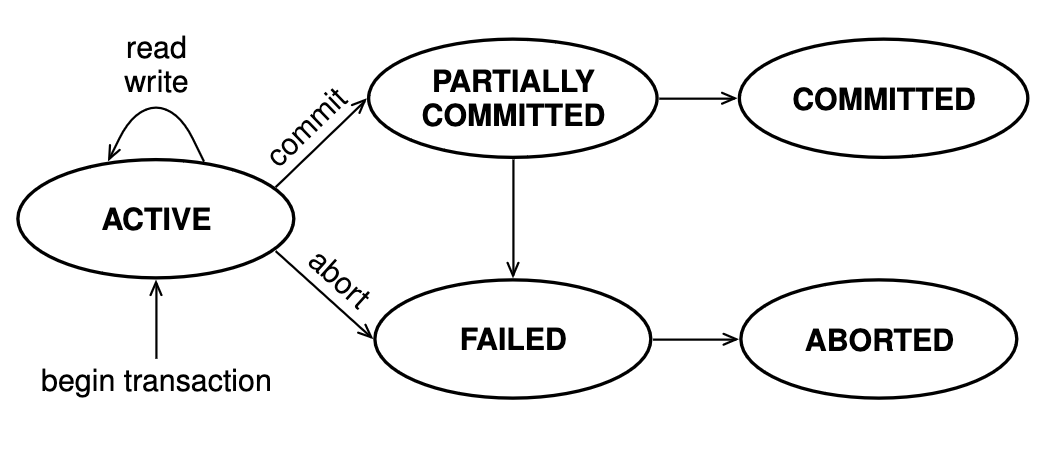
\includegraphics[width=0.5\linewidth]{img/transaction_states.png}
    \caption{State transition diagram for transaction execution.}
    \label{fig:transaction-states}
\end{figure}
To read a page ($r_i[x]$), it is brought into the buffer from the disk (if it's not already in the buffer), and then read. To write a page ($w_i[x]$), an in-memory copy is modified, which will later be written to disk when the Buffer Manager find it appropriate to do so. This delayed writing has to be compatible with Atomicity and Durability, since multiple transactions may want to write to the same page.

\section{Failures}

A database can become inconsistent because of three types of failures:
\begin{itemize}
    \item \textbf{Transaction failure}, an interruption of a transaction which does not damage the content of either the main memory or the permanent memory. A transaction can be interrupted because either it meets certain conditions, it violates integrity constraints, or the concurrency manager chooses to abort it because it is involved in a deadlock;
    
    \item \textbf{System failure}, an interruption (crash) of the system (DBMS or OS) in which the content of the main memory is lost, but the content of the content of the permanent memory remains intact. After crashes occur, the system is restarted, automatically or by an operator;
    
    \item \textbf{Media failure} (also called \textbf{disaster}), an interruption of the system in which content of the permanent memory is lost or damaged. When a media failure happens, the Recovery Manager uses a backup to restore the database.
\end{itemize}
Other than database backups, another protection from failures is represented by \textbf{log files}: these files contain lines recording each transaction operation executed in the system, including aborted transactions. For each transaction, the information written is when it starts, when it commits, when it aborts, and when it modifies a records, specifying the page the record is in, and the old and new values (called \textbf{before image} and \textbf{after image}). Each record is uniquely identified by a LSN (Log Sequence Number), assigned in a strictly increasing order.

A recovery algorithm requires an \textbf{undo} if an update of some committed transaction is stored in the database. An \textit{undo} is needed when a transaction or system failure occurs, copying the before image of the page from the log to the database. A recovery algorithm requires a \textbf{redo} is a transaction is committed before all of its updates are stored in the database (after a system failure), copying the after image in the log to the database.

The downtime of the system is given by the product between the failure rate and the recovery rate. The failure rate cannot be reduced, as we cannot know in advance if a transaction contains an error, or a system/media failure happens. The way to reduce downtime is to reduce recovery time. In practice, this is done via \textbf{checkpoints}. There's different types of checkpoints:
\begin{itemize}
    \item \textbf{Commit-consistent checkpoint}: when a checkpoint starts, the activation of new transactions is suspended, and the system waits the termination of active transactions; all ``dirty'' pages in the buffer are written to permanent memory; the checkpoint is written to the log file, and a pointer to the corresponding record is stored in a special file called \textbf{restart file}. The system then resumes normal activity. This strategy is simple but inefficient, since the system has to regularly stop.

    \item \textbf{Buffer-consistent checkpoint - Version 1}: similar to the previous type, but once the checkpoint starts, it also suspends the execution of currently active transactions. This strategy is more efficient than the previous, but it is still slow because of the buffer flushing operations.

    \item \textbf{No stop checkpoint}: once the checkpoint starts, the checkpoint is written to the log file, along with the ids of currently active transactions; a new thread is started, which scans the buffer and flushes the dirty pages it finds in parallel with the standard transactions, guaranteeing that all pages that were dirty at the beginning of the checkpoint are flushed before its end.
\end{itemize}

\subsection{Recovery from System and Media Failures}

In order to recover the database, the \textit{restart} operator is invoked, bringing the database in its committed state with respects to the execution up to the system failure, and restarting the normal system operations. The first task is done using a recovery algorithm of which a simple version will be described. This algorithm has two phases, \textbf{rollback} and \textbf{rollforward}. In the rollback phase the log is read backwards, to undo updates of transactions that were not terminated before the crash, and to find the identifiers of the transactions which terminated successfully. In particular, two sets are constructed: the \textbf{redo-list} and the \textbf{undo-list}. Until the first checkpoint record is found, these operations are done:
\begin{enumerate}
    \item If a record is (\textit{commit}, $T_i$), $T_i$ is added to the redo-list.
    
    \item If a record is an update of a transaction $T_i$ not in the redo-list, it is added to the undo-list.

    \item If a record is (\textit{begin}, $T_i$), $T_i$ is removed from the undo-list.

    \item If a record is a checkpoint (\textit{CKP}, $L$), for each $T_i \in L$ if $T_i$ is not in the redo-list it is added to the undo-list. If the undo-list in not empty, the rollback phase continues until it is completely emptied.
\end{enumerate}
In the rollforward phase, the log is read onward from the first record after the checkpoint, redoing all operations of the transactions in the redo-list.

The restart is executed at the buffer level, not on the persistent store: undos and redos are done by first loading the data in the buffer, and then pages are eventually flushed in a second time.

The algorithm described above is the standard Undo-Redo algorithm, but there exist variants:
\begin{itemize}
    \item \textbf{NoUndo-Redo}: requires that all the updates of a transaction must be in the database after the transaction has committed. It uses a \textbf{NoSteal (Pin) Policy}, where all the buffers used by transactions are pinned, and those pages will not be flushed to disk until the transaction commit. This way, no operation ever needs to be undone. It is dangerous because it pins all those pages used by the active transactions, limiting the freedom of the buffer manager.

    \item \textbf{Undo-NoRedo}: requires that all the updates of a transaction must be in the database before the transaction has committed. It uses a \textbf{Force} policy, where buffer pages used by transactions are forcibly flushed before committing. This approach has two problems: it does not work for media failures, and it is costly since it requires a lot of writes to disk.

    \item \textbf{NoUndo-NoRedo}: requires that all the updates of a transaction must be in the database neither before nor after the transaction has committed. It uses NoSteal and Force policies.
\end{itemize}
Undo-Redo uses Steal and NoForce policies.

NoUndo-NoRedo requires a way to write many pages atomically. This is done using \textbf{shadow pages}. When a transaction updates a page for the first time, a new database page is created, called \textbf{current page}, with a certain address $p$. The old page in the database is unchanged, and becomes a shadow page. The \textbf{New Page Table} (a copy of the Page Table containing all physical addresses of pages) is updated so that the first element contains the physical address $p$ of the current page. All subsequent write and read operations on that page will operate on the current page.

Once the transaction reaches the commit point, the system substitutes all shadow pages with an atomic actions: first, all the pages updated in the buffer are written to the permanent memory, while the Page Table is left unchanged; then, the descriptor of the database is updated with an atomic operation, replacing the pointer to the Page Table with that to the New Page Table, which becomes the Page Table.

There are some optimizations of the algorithm:
\begin{itemize}
    \item Setting the log granularity at a record level instead of page level;

    \item Buffering the log;

    \item Writing in pages the LSN of the last operation executed;

    \item Logging undo actions;

    \item Adding to each log entry the LSN of the previous entry for the same transaction.
\end{itemize}
\chapter{Concurrency}

When transactions are executed concurrently, their operations are often interleaved, meaning that the execution of the operations of one transaction alternates with the execution of the operations of the other. This may cause interferences that leave the system in an inconsistent state, and it is responsibility of the Concurrency Manager to prevent this from happening. We assume all transactions are consistent, so if a transaction were to be executed in isolation it would not violate any constraint. There are three types of possible conflicts arising during concurrent execution:
\begin{itemize}
    \item \textbf{Dirty Reads (Write-Read conflicts)}: one uncommitted transaction writes on some data $x$, and the other reads that same $x$ after the write operation has been completed. If the first transaction aborts, the changes to $x$ should not have had an effect on the execution of the second one.

    \item \textbf{Unrepeatable Read (Read-Write conflict)}: a transaction reads the same data $x$ twice, but between the two reads, a write operation on $x$ by another transaction is scheduled. The first transaction will read two different values of $x$, despite expecting them to be the same for both reads.

    \item \textbf{Lost Update (Write-Write Conflict)}: two transactions read the value of the same data $x$ (with no conflict), but then both update $x$ with a new value. Whichever transaction gets to update $x$ last is the one whose change will have an effect on the database, regardless of when it started w.r.t. the other one. 
\end{itemize}
A simple way to avoid interference is to allow only \textbf{serializable execution}.
\BoxDef{Serial Execution}{
An execution of a set of transactions $T = \{T_1, \dots, T_n\}$ is serial if, for every pair of transactions $T_i$ and $T_j$, all the operations of $T_i$ are executed before the ones of $T_j$, or vice-versa. 
}
However, serial execution in unpractical, since one transaction is executed at a time, stopping the others from accessing the data for potentially long periods of time. To make sure that the database stays in a consistent state, it is sufficient that the system guarantees that the execution of interleaved transactions is \textbf{serializable}.
\BoxDef{Serializable Execution}{
An execution of a set of transactions $T$ is serializable if it has the same effect in the database of some serial execution of the set of committed transactions $T' \subseteq T$.
}
Aborted transactions are ignored since they should not change the state of the database. Since serial executions are correct, any serializable execution is also correct by virtue of having the same final effect.

\section{Histories}

A transaction is a sequence of read/write operations. An \textbf{history} is used to represent the interleaved execution of multiple transactions.
\BoxDef{History}{
Let $T = \{T_1,\dots,T_n\}$ a set of transactions. A history $H$ on $T$ is an ordered set of operations such that:
\begin{itemize}
    \item The operations of $H$ are those of $T_1,\dots,T_n$;
    \item $H$ preserves the ordering between the operations belonging to the same transaction.
\end{itemize}
}
A history is an actual (or potential) execution order of the operations of a set of transactions; for example, given the transactions:
\begin{align*}
    &T_1 = r_1[x], r_1[y], w_1[x], c_1 \\
    &T_2 = r_2[y], r_2[z], c_2 \\
    &T_3 = w_3[x], w_3[y], c_3 \\
\end{align*}
a history may be:
\begin{equation*}
    H = r_1[x], r_2[y], r_1[y], w_3[x], w_3[y], w_1[x], c_1, r_2[z], c_3, c_2
\end{equation*}
In an history, two operations of different transactions can be \textbf{in conflict}, i.e., they are on the same data item and at least one of them is a write operation. In the example above, $r_1[x]$ and $w_3[x]$ are in conflict.

\BoxDef{Equivalent Histories}{
Two histories $H$ and $L$ are equivalent if:
\begin{itemize}
    \item They are defined on the same set of transactions;
    \item They produce the same final effect on the database.
\end{itemize}
}
A history is serializable if it is equivalent to a serial history. Equivalence between histories can be defined taking only into account the order of operations in conflict:
\BoxDef{c-Equivalent Histories}{
Two histories $H$ and $L$ are c-equivalent (conflict-equivalent) if:
\begin{itemize}
    \item They are defined on the same set of transactions;
    \item They have the same order of operations in conflict of committed transactions.
\end{itemize}
}
This definition of c-equivalence is motivated by the fact that the result of concurrent execution of $T_1,\dots,T_n$ depends only on the order of execution of the operation in conflict: if two operations are not in conflict, they will always have the same final result on the database regardless of their ordering.

\BoxDef{c-Serializable History}{
A history of transactions $T$ is c-serializable if it is c-equivalent to a serial history on the same transactions of $T$.
}
c-serializability always implies serializability, but not vice-versa.

Although it is possible to examine a history $H$ and decide whether or not it is c-serializable using reordering of operations, there is another simpler way to proceed based on the analysis of a particular graph derived from $H$, called \textbf{serialization graph}.
\BoxDef{Serialization Graph}{
Let $H$ be a history of committed transactions $T = \{T_1, \dots, T_n\}$. The serialization graph of $H$, denoted $SG(H)$, is a directed graph such that:
\begin{itemize}
    \item There is a node for every committed transaction in $H$;
    \item There is a directed arc $T_i \rightarrow T_j, i \neq j$, if and only if some operation $p_i$ in $T_i$ appears before and conflicts with some operation $p_j$ in $T_j$.
\end{itemize}
}
Two transactions $T_i$ and $T_j$ in $H$ are in conflict if the arc $T_i \rightarrow T_j$ appears in $SG(H)$.
\BoxDef{c-Serializability Theorem}{
A history $H$ is c-serializable if and only if its serialization graph is acyclic.
}
If the serialization graph is acyclic, a serial schedule can be obtained with a topological ordering on the graph.

\section{Serializability with Locking}

Analyzing the serialization graph can verify a posteriori if a history is c-serializable; in practice, serialization graphs are not constructed. The c-serializability theorem, however, can be used to prove that the scheduling algorithm for the concurrency control used by a scheduler is correct.

\subsection{Strict Two-Phase Locking (2PL)}

Strict Two-Phase Locking is the most commonly used scheduling protocol in commercial systems. Under this protocol, each data item used by a transaction has a lock associated with it, a \textbf{read lock} (shared), or a \textbf{write lock} (exclusive). Two rules are followed:
\begin{itemize}
    \item If a transaction wants to read (write) a data item, it first requests a shared (exclusive) lock on the data item. Before a transaction can access a data item, the scheduler first examines the lock associated with the data item. If no other transaction holds the lock, then the data item is locked; otherwise, the transaction must wait until the lock is released.
    
    \item All locks held by a transaction are released together the moment it commits or aborts.
\end{itemize}
Lock-granting policies are described by the \textbf{compatibility matrix}, where each row corresponds to a lock that is already held on an element $x$ by another transaction, and each column corresponds to the mode of a lock on $x$ that is requested (here ``S'' stands for ``shared'' and ``X'' stands for ``exclusive''):
\begin{table}[h]
    \centering
    \begin{tabular}{|c||c|c|}
    \hline
         & S & X \\
    \hline
    \hline
        S & \colorgreen{y} & \colorred{n} \\
    \hline
        X & \colorred{n} & \colorred{n} \\
    \hline
    \end{tabular}
    \caption{Compatibility matrix for shared/exclusive locks.}
    \label{tab:my_label}
\end{table}
In short, if an item has a read lock, it can receive more read locks but no write locks. If it has a write lock, no more locks of any kind can be placed.

Locks are handled by a scheduler, which tracks all locks granted to transactions and on which data items: each lock is a triple $(T, mode, x)$. When a transaction asks for a lock on an item, it is granted if possible (according to the above table), otherwise the transaction is suspended and added to a \textbf{wait queue} (hashed on the item). Once a transaction commits or aborts, all the locks it held are released, and any waiting transaction is notified according to a specific policy.

\BoxDef{Theorem}{
A strict 2PL protocol ensures c-serializability.
}

\subsection{Deadlocks}

The scheduler needs a strategy to detect \textbf{deadlocks}, situations in which a transaction $T_i$ has locked an item $A$ and requests a lock on item $B$, while at the same time, a transaction $T_j$ has locked item $B$ and requests a lock on item $A$. A deadlock occurs because none of the transactions can proceed.

\subsubsection{Deadlock Detection}

A simple strategy is using a \textbf{wait-for graph} in which each node is a transaction, and a directed edge between two transactions $T_i$ and $T_j$ means that $T_i$ is waiting for $T_j$ to release a lock on one of its objects. If a cycle occurs in the graph, a deadlock has occurred, and one of the transactions involved must abort, usually the youngest (chosen on the basis of some metric, such as newest timestamp, lowest number of locks, etc.).

In real applications, managing this graph can become very expensive. Either the existence of wait cycles may be controlled at predetermined time intervals, or the graph is not constructed and instead a timeout strategy is used: if a transaction waits to get a lock on a data item for more than \textit{timeout}, the scheduler assumes a deadlock has happened and aborts the transaction. This solution, however, causes thrashing: the system may accidentally start killing transactions which are not involved in deadlocks, in turn slowing down transaction execution. In some DBMSs (such as PostgreSQL), a shorter deadlock timeout is used instead; if this timeout expires, the system builds a local wait-for graph for that transaction, and if the graph contains a loop the transaction is killed.

\subsubsection{Deadlock Prevention}

Another strategy that instead prevents deadlocks from ever happening is the following: each transaction $T_i$ receives a timestamp $t_s(T_i)$ when it starts; if $t_s(T_i) < t_s(T_j)$, then $T_i$ is older than $T_j$. Each transaction has a priority assigned to it, such that the older is a transaction, the higher priority it has.

When a transaction $T_i$ requests a lock on a data item that is already locked on by another transaction $T_j$, two algorithms are possible:
\begin{itemize}
    \item \textbf{Wait-Die}: if $T_i$ is older than $T_j$ it waits until $T_j$ terminates, otherwise aborts.

    \item \textbf{Wound-Wait}: if $T_i$ is older than $T_j$ it aborts it, otherwise it waits until $T_j$ terminates.
\end{itemize}
In both cases, when the killed transaction is restarted, it keeps the same priority (timestamp) it had originally. Both algorithms ensure no starvation. Wait-Die tends to roll back more transactions, but those transactions are also the ones who tend to have done less work since they're younger.

Wait-Die and Wound-Wait are easier to implement than wait-for graphs, and they also tend to kill a huge amount of transaction (as opposed to wait-for graphs who only kill transactions which are presumed to be involved in a deadlock).

\section{Serializability without Locking}

The previous methods are called \textbf{pessimistic}, because they assume that operations of different transactions are very likely to conflict, and act accordingly. Methods that don't use locks are called \textbf{optimistic}: transactions are free to execute their operations, and the system only controls that no errors have happened.

One such method, used by Oracle, is \textbf{snapshot isolation}. In this solution, all reads and writes are done without locks. Each transaction $T_i$ reads the data out of a database version called \textbf{snapshot}, containing the state of all data items as they were modified by all transactions committed before it. All the write operations done by the transaction are collected in a dedicated \textbf{write set} $WS_i$ and they are visible only by $T_i$ but not other transactions. If a transaction executes a write, it can only commit if its write set does not intersect with another committed transaction's write set. If the intersection is not empty, the transaction is aborted: this is called the ``First-Committer-Wins'' rule.

This solution permits non-serializable executions.

\section{Multiple-Granularity Locking}

The locking techniques presented up until now assume that locks are taken for single records. In real applications, transactions may operate on collections of records, so these record-level locks are not enough to guarantee a consistent state of the database. On the other hand, if only table-level locks are provided by the DBMS, transactions that only write on single records will have to lock the entire table they are found in, slowing down execution.

Other techniques have been developed to support locks with different granularity (database, files, page, record, fields), such that an inclusion relationship is defined across the levels. If a transaction gets an \textbf{explicit} lock on a data object, it also has an \textbf{implicit} lock on any ``child'' object as well; i.e., if a transaction has a lock on a table, it also has a lock on its records and each record's field. Low granularity locks allow more concurrency, but also cause more lock overhead and higher deadlock probability. High granularity locks allow less concurrency, but cause less overhead and less chance of deadlock.

To manage these locks, the $S$ and $X$ locks are not enough, so a new type is introduced, called \textbf{intention locks}. If a data object is locked in an intention mode, explicit locking is done at a finer granularity. Before a transaction can acquire an explicit lock on the object, it must also already hold an intention lock on all ancestors of that object in the granularity hierarchy. The intention lock types are:
\begin{itemize}
    \item \textbf{Intentional Shared lock} (\textbf{IS}): allows the explicit locking of the object's descendants in $S$ or $IS$ mode;

    \item \textbf{Intentional Exclusive lock} (\textbf{IX}): allows the explicit locking of the object's descendants in $S$, $IS$, $X$, $IX$, or $SIX$ mode;

    \item \textbf{Shared Intentional Exclusive lock} (\textbf{SIX}): implicitly locks all descendants of the object in $S$ mode, and allows the explicit locking of the object's descendants in $X$, $SIX$, or $IX$ mode.
\end{itemize}
The need for the $SIX$ lock is justified by the fact that some transactions may want to only read an object higher in the hierarchy, but write on objects lower in the hierarchy. If only $S$ and $IX$ locks were used, the transaction would have to hold both those lock types on the object higher in the hierarchy. The compatibility table for these locks is the one below (where the rows represent locks already held, and columns are locks requested by some other transaction).

\begin{table}[h]
    \centering
    \begin{tabular}{|c||c|c|c|c|c|}
    \hline
         & S & X & IS & IX & SIX \\
    \hline
    \hline
        S & \colorgreen{y} & \colorred{n} & \colorgreen{y} & \colorred{n} & \colorred{n} \\
    \hline
        X & \colorred{n} & \colorred{n} & \colorred{n} & \colorred{n} & \colorred{n} \\
    \hline
        IS & \colorgreen{y} & \colorred{n} & \colorgreen{y} & \colorgreen{y} & \colorgreen{y} \\
    \hline
        IX & \colorred{n} & \colorred{n} & \colorgreen{y} & \colorgreen{y} & \colorred{n} \\
    \hline
        SIX & \colorred{n} & \colorred{n} & \colorgreen{y} & \colorred{n} & \colorred{n} \\
    \hline
    \end{tabular}
    \caption{Compatibility matrix of multi-granularity locks.}
    \label{tab:multi-granularity-locks}
\end{table}

A problem that arises with multi-granularity locks is \textbf{phantom locking}. Imagine two transactions, $T_1$ and $T_2$, which are executing the following operations:
\begin{itemize}
    \item $T_1$: SELECT * FROM Students
    \item $T_2$: insert into Students values (100, 'Rossi')
    \item $T_2$: commit
    \item $T_1$: SELECT * FROM Students
\end{itemize}
$T_1$ locks the table record by record. Even if strict 2PL protocol is used, this history is still possible. This is because even if $T_1$ has a lock on the data objects in the table Students, $T_2$ is not updating or deleting an existing record, but inserting a new one, and $T_1$ obviously cannot lock an object that cannot exist yet.

The same problem can be seen for the following cases:
\begin{itemize}
    \item $T_1$: SELECT * FROM Students WHERE Surname='Rossi'
    \item $T_2$: insert into Students values (100, 'Rossi')
    \item $T_2$: commit
    \item $T_1$: SELECT * FROM Students WHERE Surname = 'Rossi'
\end{itemize}
and
\begin{itemize}
    \item $T_2$: DELETE FROM Students WHERE Surname='Rossi'
    \item $T_1$: SELECT * FROM Students WHERE Surname='Rossi'
    \item $T_2$: abort
    \item $T_1$: SELECT * FROM Students WHERE Surname = 'Rossi'
\end{itemize}
In the latter case, the records on which an exclusive lock is held by $T_2$ are deleted, thus deleting the lock as well.

To fix this problem, a new protocol is introduced, extending the strict 2PL one. This protocol is called \textbf{Multi-granularity Strict 2PL}, and adds these two rules:
\begin{enumerate}
    \item A (non-root) node can be locked by a transaction $T_i$ in $S$ or $IS$ mode only if the parent is locked by $T_i$ in $IS$ or $IX$ mode;

    \item A (non-root) node can be locked by a transaction $T_i$ in $X$, $IX$, or $SIX$ mode only if the parent is locked by $T_i$ in $SIX$ or $IX$ mode. 
\end{enumerate}

\chapter{Physical Database Design}

The design of a relational database has four phases:
\begin{itemize}
    \item Requirements analysis, for the specification of data to be taken into account and the services to be implemented;
    \item Conceptual design, defining the representation of the entities of interest and their properties, associations, and integrity constraints;
    \item Logical design, defining the logical schema;
    \item \textbf{Physical design}, defining the appropriate storage structures used for the DBMS in order to guarantee the desired performances.
\end{itemize}
The information needed in order to work on the physical design of a database are:
\begin{itemize}
    \item \textbf{Statistics}: information about number of records in each relation, record size, number of pages used, distinct values per attribute, maximum and minimum values, and a distribution (if not uniform);
    \item \textbf{Workload description}: a description of critical queries and updates and their frequency, along with their respective expected performances. 
    For each critical query, this description specifies the relations and attributes used, the attributes used in selection and join conditions, and the selectivity factor of conditions. For updates, it also specifies the type (INSERT/DELETE/UPDATE).
    
    This information is usually represented using \textbf{ISUD} (Insert, Select, Update, Delete) tables: for each application, they specify the execution frequency, the percentage of data used, and the type of operation;
    \item \textbf{Knowledge about the DBMS}: data organizations, indexes, and query processing techniques supported.
\end{itemize}
Once this information is known, decisions can be made for storage structures and indexes.

\section{Database Design}

\subsection{Storage Structures}

For the storage structures, a solution can be selected from the ones seen in the first chapter: sequential, heap, hash, or index organization. Heap organization is best for small databases where insertions are more frequent than searches, sequential organization is best if it's interesting to keep static data sorted on a key, hash organization is best if the most common operation is record search by a key, and finally index organizations can both keep data sorted on a key and support efficient equality and range searches.

\subsection{Indexes}
The main goal of indexes is to avoid a relation scan when few records are looked for. Systems will usually automatically define indexes on primary and secondary keys. They can speed up searches, but they occupy memory and can slow down updates of the attributes on which they are defined, since any change to the actual records must be reflected in the index as well. In general, indexes are unnecessary for relations that occupy very few pages, or for attributes that are not very selective. The problem of selecting useful indexes does not have a trivial solution, due to the large number of possibilities, which is why most commercial systems provide tools to assist in the resolution. In the absence of such tools, we must consider which are the critical queries and which plan the optimizer chooses for them, evaluating whether an index may improve performances.

For example, we should consider defining indexes on  attributes used in queries that require sorting (OrderBy, GroupBy, Distinct, Set operations); on selective attributes in the WHERE clause, choosing the appropriate structure depending on the type of search (equality, range, multi-attribute); to improve joins with IndexNestedLoop. Indexes can be defined for single queries (local view) or for workloads (global view).

An index $I$ is unnecessary if it is \textbf{subsumed} by another $I_2$, meaning that the attributes of $I_1$ are included as prefix within those of $I_2$. For example, an index on a single attribute $A$ is subsumed by an index on $(A, B)$, and both are subsumed by an index on $(A, B, C)$.

Two indexes supporting two queries can be \textbf{merged} together into one index supporting both queries. For example, if two queries caused the creation of indexes on $(A, B)$ and $(A, C)$, respectively, they can be merged into $(A, C, B)$.

From the global viewpoint, a way to create indexes is to start by defining useful indexes on single critical queries; then, indexes that can be subsumed are removed from the set of all indexes, and the benefit/cost ratio is evaluated for the remaining ones.

\paragraph{Use of Clustered Indexes} Clustered indexes are best used for equality and range searches on non-key attributes, even if the selectivity factor is not very restrictive. It can also be useful for queries in which data must be sorted (usually when the query has a GroupBy).

\paragraph{Multi-Attribute Indexes} Indexes defined on multiple attributes at once can be used for queries with equality-equality searches, or equality-range searches. It's important to consider the order in which the index attributes are specified: the first one should be the one used for mostly equality searches.

Since each element in the index contains several attributes, there is a greater chance that the optimizer will generate plans using only the index. However, multi-attribute indexes must be updated each time an update is done on an attribute on which it is defined, and occupies more memory than an index on a single attribute.

\paragraph{Indexes for Join} Clustered indexes on a non-key join attribute of the internal table can improve the performances of an IndexNestedLoop, since it requires an IndexFilter as its inner operand.

\paragraph{Index-Only Plans} In some cases, it is possible to execute Index-Only plans for a query, i.e., plans in which only indexes are accessed instead of the actual data. These plans can be generated if an index has been defined on the attributes appearing in the SELECT DISTINCT clause, or the GROUPBY clause.

Also, if indexes are defined for the inner operand on a foreign key needed for a join, the plan can use IndexOnlyFilter instead of IndexFilter.

\section{Database Tuning}

Database tuning includes all activities carried out to meet requirements regarding the performance of database applications. By ``performance'', we refer to runtime performance, so \textbf{throughput} (number of operations completed in a unit of time), \textbf{response time} (time to execute an application), and \textbf{resource consumption} (temporary or permanent memory used). For each potential decision to be taken, the trade-off between its costs and benefits is evaluated. Costs include any monetary cost (hardware, software), working hours, technical costs, while benefits include any improvement in performances (sometimes quantified in monetary effects, although often not easy to do). \\
Tuning considers the following aspects:
\begin{itemize}
    \item Applications: user queries and transactions;
    \item DBMS: configurations, parameters, database schema, storage structures;
    \item Operating system: system parameters and configuration for I/O, network communication;
    \item Hardware: components used for CPU, main and permanent memory.
\end{itemize}
A basic idea at the basis of database tuning is Pareto principle: by applying 20\% of the effort one can achieve 80\% of the desired effects, meaning that a fully optimized system may be unnecessary, and the process should instead focus on smaller (but with significant improvements) changes.
\begin{figure}[h]
    \centering
    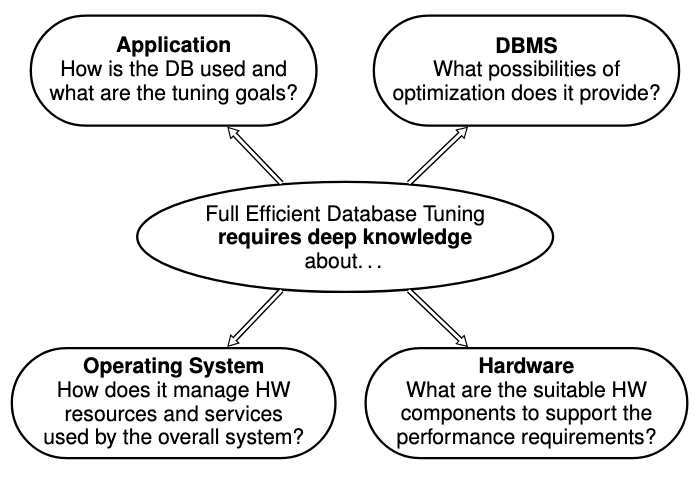
\includegraphics[width=0.5\linewidth]{img/quadrilemma.png}
    \caption{The DBMS tuning \textit{quadrilemma}.}
    \label{fig:quadrilemma}
\end{figure}
This is a complex and continuous process which involves different professional figures:
\begin{itemize}
    \item Database and applications designers, who have knowledge about applications and the DBMS, but may have little knowledge about OS or hardware;
    \item Database administrators, who have good knowledge about DBMS, OS, and hardware, and may have little knowledge about applications;
    \item Database experts, who usually have strong knowledge in DBMS, OS, and hardware, but very limited knowledge about applications.
\end{itemize}

\subsection{Index Tuning}

The initial choice of indexes could be revised for different reasons: the workload of the database may reveal that some queries initially considered critical are not actually executed that often, while others which had initially been thought of as infrequent turned out to be important. In some cases, the optimizer does not generate the physical plan that was expected. Either way, changing indexes can improve performances.

\subsection{Query Tuning}

If the optimizer does not transform SQL queries, they can be explicitly rewritten with two set of rules:
\paragraph{Semantically Equivalent Rewriting}
\begin{itemize}
    \item If a query has an Or condition, it may be rewritten using an Union of different queries, or using the In predicate specifying both conditions;

    \item If a query has an And of different predicates, it can be rewritten as a condition with Between (if the values in the predicates describe a range);

    \item Avoid arithmetic expressions on attributes used in conditions (e.g., instead of writing ``Salary*2 = 100'', write ``Salary = 50'', because for the first condition the optimizer may not use an index);

    \item Subqueries can be rewritten as joins;

    \item Avoid temporary views. If the optimizer cannot rewrite the query without views, the physical plan will have an higher cost;

    \item Redundant Having and GroupBy should be removed.
\end{itemize}

\paragraph{Semantically Non-Equivalent Rewriting}
\begin{itemize}
    \item Avoid useless Distinct and OrderBy clauses;
    
    \item Avoid cartesian products.
\end{itemize}

\subsection{Transaction Tuning}

Another cause of inefficiency in DBMS is the way transactions are programmed. They should be as short as possible to reduce the duration of the locks they hold over data objects (although as seen before many modern systems use more sophisticated locks instead of read-write locks, so this problem is not as big), and they should not block data during database loading and during read-only transactions. Complex transactions should be split into smaller ones. Also, if a transaction has to stop because user input is being asked, it should commit and restart after input has been received. Each transaction should have the appropriate block granularity (record, page, table, etc.), as well as the appropriate isolation level:
\begin{itemize}
    \item \textbf{READ UNCOMMITTED}: the reads of records are performed without requesting any locks, so dirty reads are possible;

    \item \textbf{READ COMMITTED}: the transaction obtains locks on records, released right after reading, and exclusive locks before writing (held until the end). This prevents dirty reads but not non-repeatable reads.

    \item \textbf{REPEATABLE READ}: the transaction holds both read and write locks on records released at the end. This avoids     \item \textbf{READ COMMITTED}: the transaction obtains locks on records, released right after reading, and exclusive locks before writing (held until the end). This prevents dirty reads but not non-repeatable reads, but introduces the problem o \textbf{phantom records}: for example, if a transaction reads a set of records from a table which satisfy a condition $\psi$, and right after a second transaction writes a new set of records in that table with also satisfy $\psi$, the first transaction will never see those new records.

    \item \textbf{SERIALIZABLE}: the default isolation level, where read and write locks are of different sizes. Any read lock on a table will be in conflict with any update. It avoids all problems seen before, but reduces the number of concurrent transactions executable per unit of time.
\end{itemize}
Commercial DBMS don't necessarily provide all previous levels of isolation, or may have different default levels. Also, some of them provide the SNAPSHOT isolation level.

\subsection{Logical Schema Tuning}

If the physical design is not able to provide adequate performances, it may be necessary to modify the logical schema, using two types of restructuring: \textbf{partitioning} and \textbf{denormalization}.

\paragraph{Partitioning}

Partitioning can be either vertical or horizontal.

\textbf{Vertical partitioning} reduces the volume of data transferred from/to permanent memory and cache, splitting a relation separating its attributes into two sets, such that one set should contain the most frequently accessed attributes. Each partition will still have the primary key of the original relation as a subset of its attributes.

\textbf{Horizontal partitioning} reduces the cost of accessing a large relation by splitting it into sets of records, separating frequently accessed records from the others. Each partition will have all the original attributes of a disjoint subset of the original records.

\paragraph{Denormalization}

Normalization is the process of decomposing a table into smaller ones to reduce redundancy; denormalization is the opposite, so the process of adding columns to tables to improve the performance of read-only queries. This is useful when two or more tables are often read after joins, so instead of having to compute it every time, their information can be stored together in a single table.

\section{DBMS tuning}

If all else fails, the database system must be tuned. The most important things to consider can be divided into three levels that interact with each other:
\begin{itemize}
    \item \textbf{Transaction Management}: intervening on parameters such as log storage, frequency of checkpoints and dumps, etc. The more frequent they are, the faster the database can be fully restarted after a system failure or disaster, but the system performances also degrade, since they subtract resources from normal activity;

    \item \textbf{Database Buffer Size}: if the buffer is larger, performance of application improves, but it shouldn't be so big id does not fit in main memory;

    \item \textbf{Disk Management}: adding disks or using RAIS systems if disk I/O is a bottleneck, adding more memory, or using a faster processor;

    \item \textbf{Parallel Architectures}: this is an issue that strictly depends on the system in use.
\end{itemize}
An alternative is database \textbf{self-tuning}.
\chapter{Decision Support Systems}

Decision support systems are a type of \textbf{information system}. An information system is an organized collection of resources, people, and procedures finalized to collect, store, process and communicate information needed to support the on-going activities. Information can be represented as images, text, audio, or really any kind of data.

Traditional applications that use databases are called \textbf{OLTP} (\textbf{On Line Transactional Processing}), while decision support applications are called \textbf{OLAP} (\textbf{On Line Analytical Processing}). The key difference between the two is that OLTP systems are used for mostly day-by-day operations, using transactions, while OLAP systems are used to analyze the data to try and extract some hidden knowledge without updating the data. Table \ref{tab:oltp-vs-olap} compares the two in more detail.
\begin{table}[ht]
    \centering
    \small
    \begin{tblr}{
    row{even} = {BrickRed!10},
    columns={130pt, c, m},
    column{1}={75pt}}
    \hline
         & \textbf{OLTP} & \textbf{OLAP} \\
    \hline
    \hline
        \textbf{Function} & Operations & Decisions  \\
        \textbf{Users} & Operatives (clerk, IT professional) & Knowledge workers (managers, analysts) \\
        \textbf{Detail} &  Analytic & May be aggregated \\
        \textbf{Usage} & Repetitive & Ad hoc \\
        \textbf{Data} & Current & Historic \\
        \textbf{Data origin} & Internal & Internal and external \\
        \textbf{Items per operation} & Few (tens) & Many (millions) \\
        \textbf{Updates} & Frequent, small & Rare, massive \\
        \textbf{Stored in} & Database & Data Warehouse/DSS \\
    \hline
    \end{tblr}
    \caption{Comparison between OLTP and OLAP systems.}
    \label{tab:oltp-vs-olap}
\end{table}
While in traditional systems there is usually only a single database containing all the information, in DSS there are multiple data warehouses, one for each analysis.

\section{Data Warehouses}
More formally, a data warehouse can be defined as follows:
\BoxDef{Data warehouse}{
A data warehouse is a subject-oriented, integrated, non-volatile, and time-varying collection of data in support of management's decisions.
}
\begin{itemize}
    \item \textbf{Subject-oriented} means that data is stored by subject, not by applications, unlike traditional databases.
    
    \item \textbf{Integrated} means that data is gathered from a variety of sources and merged.
    
    \item \textbf{Non-volatile} means data is not changed interactively, but may be updated periodically.

    \item \textbf{Time-varying} means that data is assumed to be historical, collected over a long period of time, not necessarily up-to-date, in order to gather knowledge about the operations to be analyzed.
\end{itemize}

\subsection{Architecture}
The term ``data warehousing'' is used to refer to the process of organizing data in a data warehouse to allow end users to analyze it with business intelligence applications. The most common architecture is a three-layer one, composed of the \textbf{data sources}, \textbf{data staging}, and \textbf{data warehouse}.

The data warehouse is loaded with data extracted via \textbf{ETL} (\textbf{Extract, Transform, and Load}) applications from the many different sources of data in the previous layer, bringing them into a consistent form and performing any kind of cleaning needed, and finally storing them into the data staging. The complexity of data staging depends on the quality of the data sources.
\begin{figure}[ht]
    \centering
    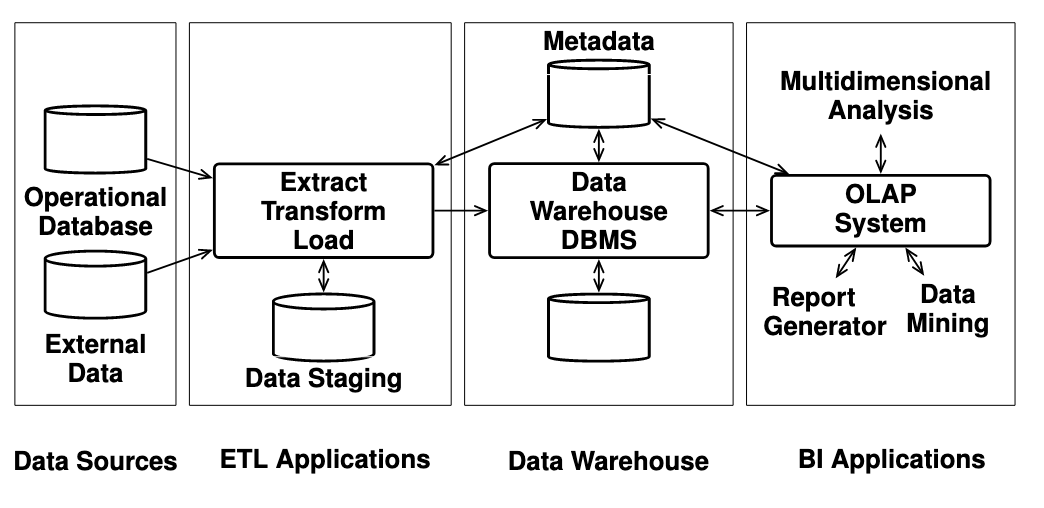
\includegraphics[width=0.5\linewidth]{img/three_layer_architecture.png}
    \caption{Scheme of a data warehouse architecture.}
    \label{fig:enter-label}
\end{figure}

\subsection{Modeling}

The creation of a data warehouse takes place gradually, at different levels of abstraction: it starts with a conceptual model, then a logical model, and finally, a multidimensional cube model.

\subsubsection{Conceptual Model}

The \textbf{Dimensional Fact Model} is a graphical conceptual model for data warehouses. It allows the representation of the following basic information:
\begin{itemize}
    \item \textbf{Facts}: the most important abstraction mechanism is the collection of facts, which are the observations of the performance of a business process. They are usually transactions or events (e.g., sales, clicks, complaints, visits), and may be \textbf{periodic} (one fact for a group of transactions made over a period of time), or \textbf{accumulating} (one fact for the entire life of the event, evolving over time).
    
    Facts are modeled by \textbf{fact tables}, each of which is a rectangle divided in two parts, one containing the fact name, and the other containing the measures.
    
    \item \textbf{Measures}: measures are quantitative information whose aggregation is of interest. The aggregation function is often the sum, but may also be a count, average, max, min, and so on.

    Measures are specified inside the fact tables.
    
    \item \textbf{Dimensions}: dimensions give facts a context: they explain ``who, what, why, when, where'' a fact is happening. A dimension can be described as a set of attributes used to qualify, categorize, or summarize facts in reports.

    Dimensions are represented by a circle connected to the fact table with a straight line, and one additional circle for each attribute of that dimension.
\end{itemize}
In the presence of dimensions, an hierarchical relationship can be modeled among them. For example, imagine a fact table with dimensions relating to dates (Year, Quarter, Month, Week, Day). A hierarchy can be constructed (Day $\rightarrow$ Week $\rightarrow$ Month $\rightarrow$ Quarter $\rightarrow$ Year) such that each element is more general than those coming before it, and less general than those after. In this case, Month is more general than Day, but is less general than Quarter. Formally, each arc of the hierarchy models a \textbf{functional dependency} between the two attributes. Graphically, hierarchies are represented as a directed tree, rooted in a dimension, and with the leaves representing the most general dimensions.

The presence of a hierarchy increases the possibilities of data analysis from different perspectives (so-called multidimensional analysis). If we already analyzed sales by year, we can also analyze them at a deeper level, considering months or days.
\begin{figure}[ht]
    \centering
    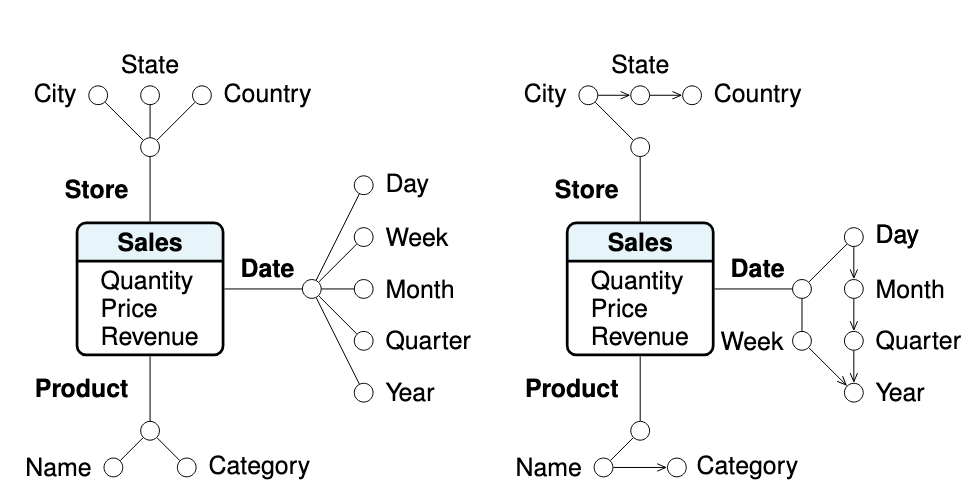
\includegraphics[width=0.75\linewidth]{img/hierarchies.png}
    \caption{Conceptual design without and with hierarchies.}
    \label{fig:hierarchies}
\end{figure}

\subsubsection{Relational Model}

A conceptual model can be transformed into a relational schema by applying a set of mapping rules. The most common schemas are the star schema, the snowflake schema, and the constellation schema.

In a \textbf{star schema}, the fact table is placed a the center, and a foreign key is added for each dimension. Dimensions are also transformed into tables (simply adding all the attributes, without considering hierarchies), and connected to the fact table with a one-to-many relationship.

A \textbf{snowflake schema} is similar to a star schema, but some dimension tables are also normalized, splitting the data into additional tables.

A \textbf{constellation schema} has multiple fact tables that share dimension tables.

\begin{figure}[ht]
    \centering
    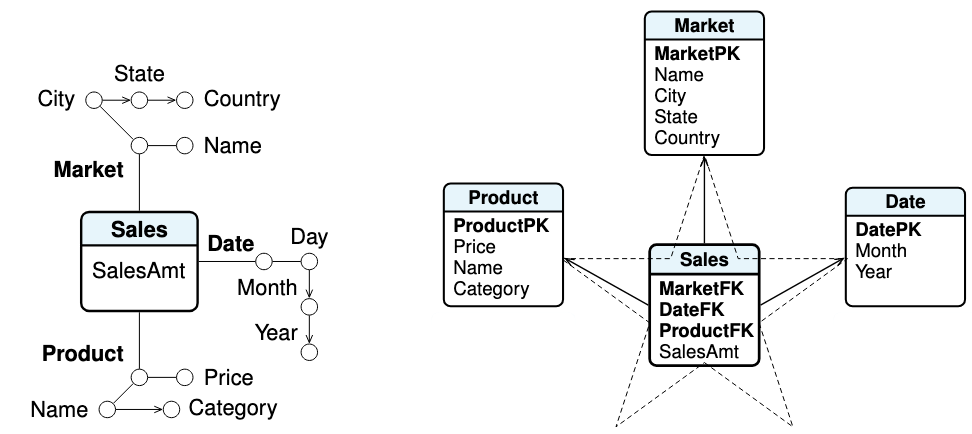
\includegraphics[width=0.65\linewidth]{img/star_schema.png}
    \caption{Star schema.}
    \label{fig:star-schema}
\end{figure} 
\begin{figure}[ht]
    \centering
    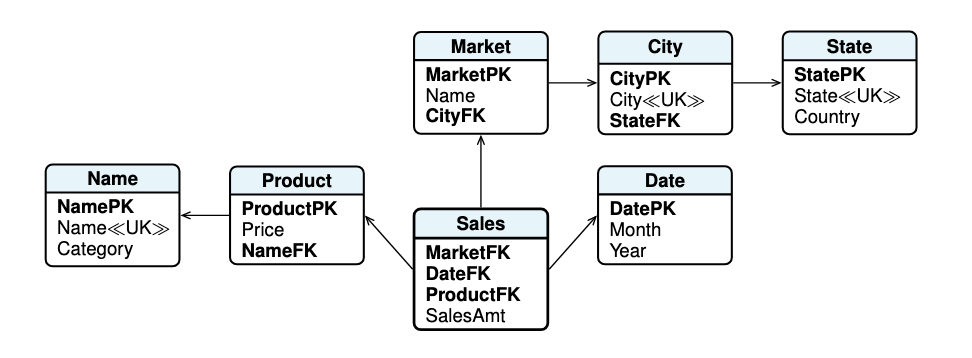
\includegraphics[width=0.65\linewidth]{img/snowflake_schema.png}
    \caption{Snowflake schema.}
    \label{fig:snowflake-schema}
\end{figure}
\begin{figure}[H]
    \centering
    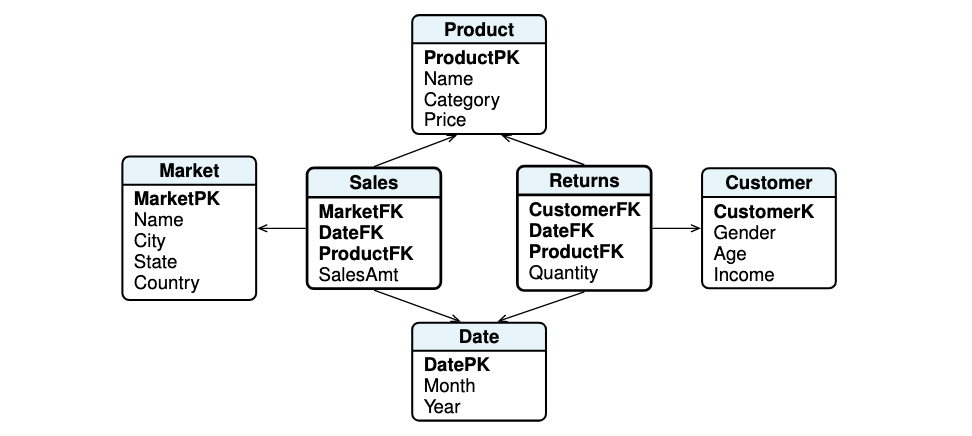
\includegraphics[width=0.65\linewidth]{img/constellation_schema.png}
    \caption{Constellation schema.}
    \label{fig:constellation-schema}
\end{figure}

\subsubsection{Multidimensional Cube Model}

A \textbf{multidimensional data model} (data cube) represents facts with $n$ dimensions as points in an $n$-dimensional space. A point (fact) is identified by the values of its dimensions, and has an associated set of measures. This view is an intuitive way to think about OLAP queries and their results.

For example, imagine a fact table with information about store sales. Each record in the original data has three attributes: a store id, a product id, and an associated quantity. We can see this data as 2-dimensional: the two dimensions are the store and the product id, while the measure is the quantity.
\begin{figure}[ht]
    \centering
    \begin{minipage}{0.49\textwidth}
        \centering
        \begin{tblr}{
            row{even} = {BrickRed!10}
        }
        \hline
           \textbf{StoreId}  & \textbf{ProductId} & \textbf{Qty} \\
        \hline
        \hline
            S1 & P1 & 300 \\
            S2 & P1 & 500 \\
            S3 & P1 & 50 \\
            S1 & P2 & 300 \\
            S2 & P2 & 10 \\
            S3 & P2 & 30 \\
            S1 & P3 & 40 \\
            S3 & P3 & 20 \\
        \hline
        \end{tblr}
        \caption{Fact table.}
    \end{minipage}
    \hfill
    \begin{minipage}{0.49\textwidth}
        \centering
        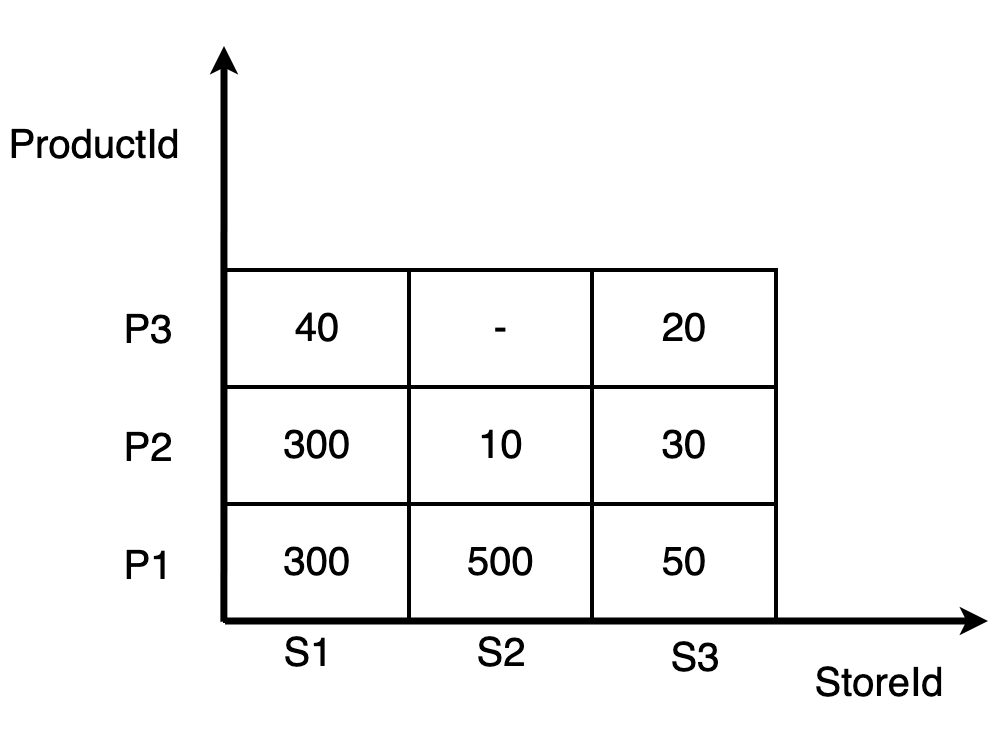
\includegraphics[width=\linewidth]{img/datacube.png}
        \caption{Example data cube.}
    \end{minipage}
\end{figure}
Obviously, this is a very simple case. In real applications, the number of dimensions can be higher than 2 or 3, so the data cube cannot be visualized in its entirety. These cubes can be manipulated via a specific geometric language, of which we can define these basic operations:
\begin{itemize}
    \item \textbf{Slice}: slicing means ``cutting'' the cube by selecting on a specific value for one dimension.

    \item \textbf{Dice}: dicing is similar to slicing, but selects on two or more dimensions.

    \item \textbf{Pivot}: pivoting performs a rotation of the data axes, providing an alternative presentation of the data.

    \item \textbf{Roll-up}: rolling-up compresses the cube across a dimension, summarizing the information provided bu that dimension. It can be seen as similar to a GroupBy done on all other dimensions not involved in the roll-up.

    \item \textbf{Drill-down}: it is the reverse of roll-up. It produces more detailed data across a dimension.
\end{itemize}

Assume that, given a data cube, eacj dimension is extended with an additional value, ``*'', representing summarization along that dimension. Then, the cube can be extended with borders containing the values of the sum along each possible combination of dimensions. When we select a subcube by specifying a dimension instead of its value (e.g., (StoreId, *)), we get a roll-up of the original data across all other dimensions, called \textbf{cuboid}.

An order relation can be defined between cuboids: $C1 \preceq C2$ if $C1$ can be computed from $C2$. This order is visualized using a \textbf{data warehouse lattice}. In the example below, we can see how the cuboid (StoreId) can be computer from (StoreId, ProductId), but (StoreId, ProductId, DateId) cannot be computed from (StoreId, ProductId). So, how do we choose which of these cuboids to store? Obviously, the source data allows us to compute all other cuboids. However, if the queries most commonly executed only consider a subset of the dimensions, we may store those (or store one of those above them).

\begin{figure}[ht]
    \centering
    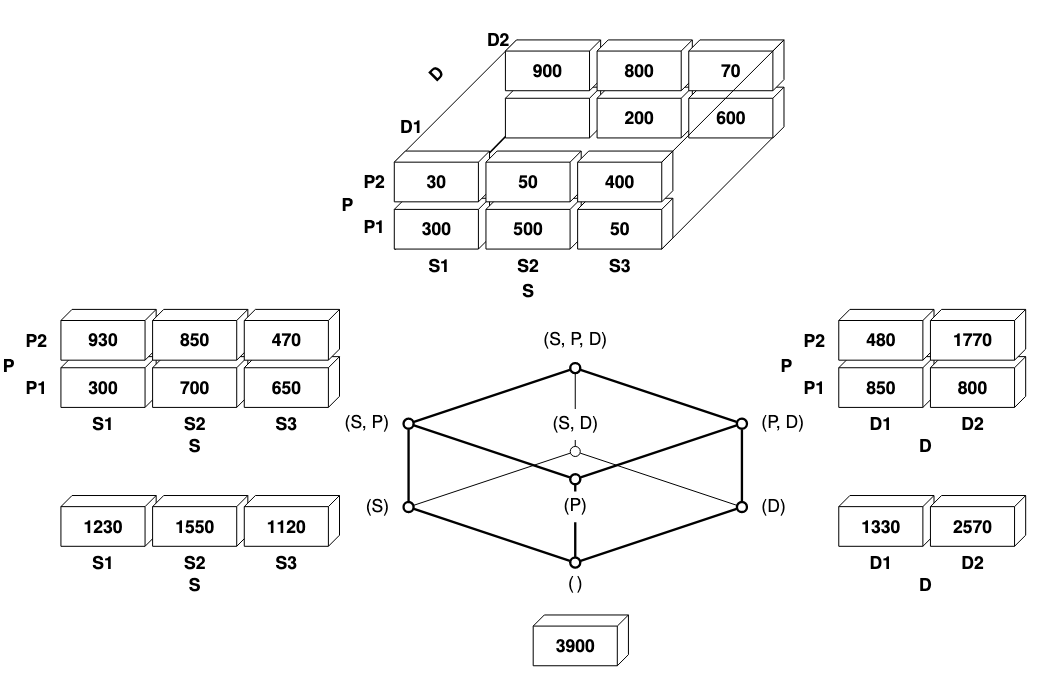
\includegraphics[width=0.8\linewidth]{img/lattice.png}
    \caption{A data warehouse lattice. The data cube it corresponds to has three dimensions: StoreId, ProductId, and Date.}
    \label{fig:lattice}
\end{figure}
\chapter{Column Databases}

\textbf{Column-oriented systems} (also known as \textbf{column-stores}) are a type of DBMS which store data by column instead of by row. By storing each column separately on disk, queries can read just the attributes they need, without having to read entire rows from disk and then discard what's not needed, which is also useful since physical query plans can be executed one-block-at-a-time (also called \textbf{vectorized execution}) instead of one-tuple-at-a-time, loading multiple records at once for each operator (enough to fill the cache). When compression is considered, columns are easier to compress than rows.
\begin{figure}[h]
    \centering
    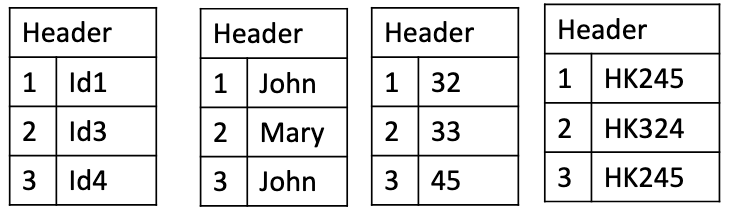
\includegraphics[width=0.5\linewidth]{img/column-store.png}
    \caption{Example of a column-store.}
    \label{fig:column-store}
\end{figure}

They've recently risen in popularity, for reasons related to changes in both applications and technology. Lately, most tasks have become analytical instead of transactional: transactional systems require efficient ways to insert or remove elements, but analytical ones not so much, and instead need efficient ways to read information (which is often a lot). As time goes on, caches become bigger, RAMs become faster, while disk performances change very little. The focus should be on reducing the accesses to disk and instead hold as much information in main memory. Also, the time between transfer time and seek time has widened, so data is often read sequentially. Finally, modern CPUs do instruction pipelining, so ideally function calls should be reduced to a minimum in order to allow the pipeline to execute operations efficiently; they also can execute the same operation in parallel on different parts of the same data structure (SIMD (Single Instruction Multiple Data) parallelism).

The basic trade-off of column-stores can be explained with a simple example. Imagine we have to read a record of 5 attributes. Using row-stores, we'd only have to read the page that contains that record, while with column-stores we'd have to read 5 pages (one per column). If instead we have to read a thousand consecutive tuples of 20 attributes out of which we're interested in 5 of them, then (assuming each page can contain the equivalent of 1000 fields) with a row-store we'd have to read 20 pages, while with a column-store we still have to read only 5 pages. In general, column-stores are advantageous for systems in which reads involve a lot of tuples ($> 1000$) on a restricted set of attributes.

The biggest challenges of column-stores are reconstruction of the tuples, which require a join, and tuple insertion, which takes many I/O operations since all different columns must be updated with the new values (although this is not a big issue in OLAP systems). These problems are exacerbated if the data is compressed.

\section{Storing Columns}

There's two choices in how to store columns. The traditional one is to store them in \textbf{RID order} (as shown in the previous picture): tuples can be reconstructed using a sort-merge-like algorithm, scanning columns in parallel. There's no need to explicitly store RIDs, since they can be inferred as the position of an element within the column.

Another choice is to store them in \textbf{value order}, i.e., they are kept sorted on the value of the tuples. It is extremely convenient for compression via Run Length Encoding, and also permits efficient range searches. This method requires to explicitly store the RIDs. The basic solution is to store them the same way an inverted index does: each value is associated with the list of RIDs which contain it; however, this negates the possibility of compressing the data via RLE, and tuple reconstruction requires an index-nested-loop-like random access algorithm.

Instead of using an inverted index structure, two separate data structures can be used. The first one lists all the values, each followed by the total number of records which have that value (the information is compressed via RLE). The second one is a join index, which specifies the correspondence between the first data structure and some other RID-sorted column.

Overall, using a basic inverted index-like structure is better if we're interested in reconstructing the original tuples; the second method is better if data is going to be kept as separated columns and not reconstructed.

\subsection{C-Store Projections}

The solution used by C-Store (an early column-oriented DBMS) stores each column in a separate file, using a column-specific compression method, and sorting the values according to some attribute in the table. Each column can be stored several times in different sort orders: groups of columns sorted on the same attribute are called \textbf{projections}. If there are sets of columns that are very often requested together, and the query has range searched done on one specific attribute, they can be grouped in a projection and kept sorted on that attribute. The attribute chosen for sorting will also be able to be compressed and allow no-cost GroupBys. If there's other projections sorted on that same attribute, the join done on the other columns is also more efficient (can be done via sort-merge).

Different projections can have overlapping columns. If there's a lot of them, many queries will find their optimal projection, but updates will be slower. To reconstruct the entire table, either a join is done between the different projections using join-indexes, or a big projection is defined to include all columns, capable of answering any query.

\section{Compression}

There have been several research studies that evaluate the performance of different compression algorithms. Some of them can be used on both row and column-stores, while others are specific to column-stores since they allow compression symbols to span across multiple consecutive values.

\paragraph{Run-length Encoding}
RLE compresses runs of the same value in a column to a compact singular representation. Each run is replaced with a triple: (value, starting position, run length). Alternatively, the starting position can be discarded, if we're not interested in that information (for example, if we want to do binary searches on the compressed data).

\paragraph{Bit-Vector Encoding}
Bit-vector encoding compresses columns by representing it with a set of bit vectors, one for each distinct value. Each bit corresponds to a position in the column: if the $i^{th}$ bit is equal to 1, the $i^{th}$ position contains that value, while a 0 means the absence of it. This compression is only useful if the number of distinct values is low.

\paragraph{Dictionary Encoding}
Dictionary encoding is similar to bit-vector encoding, but it maps each value in the column to a different integer, and then represents the column as the sequence of those integers.  It is used for cases in which the datatype of the values requires an high number of bits (strings, usually), so rewriting them as integers will optimize queries. 

\paragraph{Difference Encoding}
When values of a column represent some continuous function, a common way of compressing them is using difference encoding: only the first value is stored, and all the other ones are replaced with the difference with that first one.

\paragraph{Frame of Reference}
Similar to difference encoding, but used when data is stored in multiple pages. Each page is compressed as the first value followed by all differences.

\paragraph{Frequency Partitioning}
With frequency partitioning, similar values are put in the same page; each page is compressed via bit-vector or dictionary encoding.

\subsection{Operating on Compressed Data}

Using compressed data requires some modifications to the query execution engine. RLE encoded data can be operated upon without decompression, as long as there is information about the runs' starting positions. Dictionary encoding also allows range queries for range queries. Bit-vector encoding allows any bit operations on sets.

For any other compression algorithm (or any other operation not included above), tuples must be reconstructed, via either \textbf{early materialization} or \textbf{late materialization}.
\begin{itemize}
    \item Early materialization simply rebuilds the part of the table the query operates on by scanning and joining all the necessary columns, and then using relational algebra.

    \item Late materialization uses column algebra to operate on one column at a time, without needing to reconstruct the table. Each column has two elements: the set of object IDs and the other a string or integer. The operations defined for late materialization are:
    
        $\textbf{select}(\textit{bat}[H,T] AB, \textit{bool} *f(\dots, pi, \dots)) : \textit{bat}[H, \textit{nil}] \\
        = \langle [a, \textit{nil}] | [a,b] \in AB \land f(b, \dots, pi, \dots) \rangle \\
        \textbf{join}(\textit{bat}[T1, T2] AB, bat[T2, T3] CD, \textit{bool} *f(\dots, pi, \dots)) : \textit{bat}[T1,T3] \\
        = \langle [a, d] | [a,b] \in AB \land [c,d] \in CD \land f(b, \dots, pi, \dots) \rangle \\
        \textbf{reconstruct}(\textit{bat}[H,nil] AN, \textit{bat}[H,T] AB) : \textit{bat}[H,T] \\
        = \langle [a,b] | [a,b] \in AB \land [a, nil] \in AN \rangle \\
        \textbf{reverse}(\textit{bat}[H,T] AB) : \textit{bat}[T,H] \\
        = \langle [b,a] | [a,b] \in AB \rangle \\
        \textbf{voidtail}(\textit{bat}[H,T] AB) : bat[H,\textit{nil}] \\
        = \langle [a,\textit{nil}] | [a,b] \in AB \rangle \\
        \textbf{group}(\textit{bat}[\textit{oID}, T] AB) : \textit{bat}[\textit{oID}, \textit{oID}] \\
        = \{[a,o] | o = id_{AB}(b) \land [a,b] \in AB \} \\
        \textbf{sum}(\textit{bat}[\textit{oID}, \textit{int}] AB) : \textit{bat}[\textit{\textit{oID}, \textit{int}} \\
        = [\textit{nil}, \sum\{i | [o,i] \in AB\}]$
\end{itemize}
\begin{figure}[h]
    \centering
    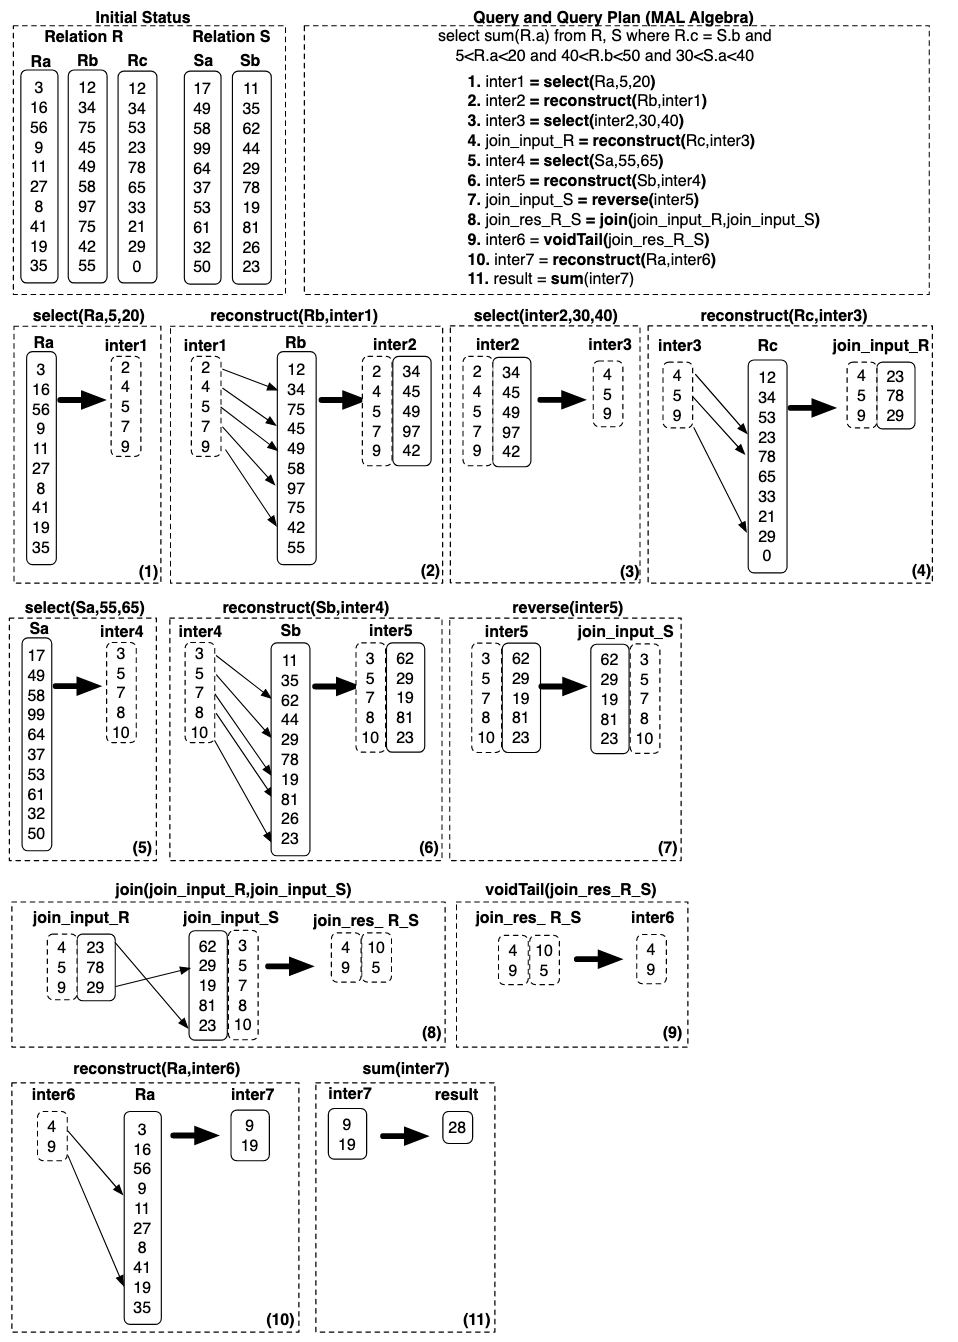
\includegraphics[width=0.75\linewidth]{img/late_materialization.png}
    \caption{Example of late materialization.}
    \label{fig:late-materialization}
\end{figure}

A binary table (``bat'') can be represented in many ways; the result of a select may just be a bitmap, and the result of a reconstruct may be a bitmap in front of the original column.

\section{Column Operations}

\subsection{Column Join}

Since columns avoid using indexes, the algorithms used to join them are HashJoin, SortMerge, or main memory join (since columns are often small enough to fit in main memory). The output of the join is a set of pairs of positions in the input relations for which the predicate succeeded. These pairs can be stored in the form of join indexes, which are often much smaller than the original columns, making subsequent operations faster.

Still, only the positions of the outer relation will be sorted, while the ones in the inner one will not, so accessing those elements will require a lot of jumps in the storage. One solution is to use the \textbf{Jive join}. This algorithm is one-operator-at-a-time, does a single read of the input relations, only blocks where one tuple that is named in the join index is present are read, and returns a result in column form (unsorted). Assume we have two tables, $R$ and $S$, both with their respective record IDs and a set of attributes, out of which only one is the join attribute:
\begin{gather*}
    R(RID, A, B), \ S(SID, BB, C) \\
    \pi_{ABC}(R \bowtie_{B=BB} S) 
\end{gather*}
Assume we also have a join index:
\begin{equation*}
    JI = \pi_{RID, SID} (R \bowtie_{B=BB} S)
\end{equation*}
Also, let $N_{pag}$ be the number of pages in the projected and semijoined $S$ plus the number of pages in the join index, then:
\begin{equation*}
    2*N_{pag} < B*B
\end{equation*}
There's no limit on $R$. To explain how the algorithm works, it is best to use an example. We have two tables:
\begin{figure}[H]
\centering
    \begin{minipage}{0.49\textwidth}
    \centering
        \begin{tabular}{|c|c|}
        \hline
            1 & Johnson \\
        \hline
            2 & Jones \\
        \hline
            3 & Johnson \\
        \hline
            4 & Doe \\
        \hline
            5 & Smith \\
        \hline
        \end{tabular}
    \end{minipage}
    \hfill
    \begin{minipage}{0.49\textwidth}
    \centering
        \begin{tabular}{|c|c|}
        \hline
            1 & Smith \\
        \hline
            2 & Johnson \\
        \hline
            3 & Williams \\
        \hline
            4 & Jones \\
        \hline
        \end{tabular}
    \end{minipage}
\end{figure}
\noindent The join produces the following join index:
\begin{table}[H]
    \centering
    \begin{tabular}{|c||c|}
    \hline
        1 & 2 \\
    \hline
        2 & 4 \\
    \hline
        3 & 2 \\
    \hline
        5 & 1 \\
    \hline
    \end{tabular}
\end{table}
\noindent As it can be seen, the outer relation RIDs are sorted. To sort the inner relation ones, we add an additional column to that list, containing an increasing sequence of integers:
\begin{table}[H]
    \centering
    \begin{tabular}{|c||c|}
    \hline
        2 & 1\\
    \hline
        4 & 2\\
    \hline
        2 & 3\\
    \hline
        1 & 4\\
    \hline
    \end{tabular}
\end{table}
\noindent This output is then sorted by the list of RIDs, causing the newly added column to be out of order:
\begin{table}[H]
    \centering
    \begin{tabular}{|c||c|}
    \hline
        1 & 4\\
    \hline
        2 & 1\\
    \hline
        2 & 3\\
    \hline
        4 & 2\\
    \hline
    \end{tabular}
\end{table}
\noindent The column from the inner table is scanned in order with values at the (now sorted) list of positions extracted and added to the current data structure:
\begin{table}[H]
    \centering
    \begin{tabular}{|c||c|c|}
    \hline
        1 & 4 & Smith \\
    \hline
        2 & 1 & Johnson \\
    \hline
        2 & 3 & Johnson \\
    \hline
        4 & 2 & Jones \\
    \hline
    \end{tabular}
\end{table}
\noindent And finally, the data structure is sorted by the added column, reverting it to the original join order:
\begin{table}[H]
    \centering
    \begin{tabular}{|c||c|c|}
    \hline
        2 & 1 & Johnson \\
    \hline
        4 & 2 & Jones \\
    \hline
        2 & 3 & Johnson \\
    \hline
        1 & 4 & Smith \\
    \hline
    \end{tabular}
\end{table}
\noindent Now, all columns can be iterated through sequentially, at the cost of two sorts of the join output data. The sorting is done by using $2*k$ buffers to create $2*k$ files with the join index and temporary sorted join index.

\subsection{Column GroupBy and Aggregation}

GroupBy is typically hash-based, unless the input is already sorted according to the groupby attributes. Aggregation exploit the column layout very efficiently: they can work on only the relevant column with tight for loops.

\subsection{Column Insert, Update, Delete}

Insertion is very expensive in column-stores, because inserts must update all columns, and if the columns are ordered, the insertion must also respect the ordering. Also, systems such as C-Store use a lot of duplication, increasing the cost even further. The same problems hold for updates and deletes.

A solution is to use differential files, stored in memory, so that all operations can be done all at once. Some database systems (such as C-Store) handle updates by splitting their architecture into a \textbf{read-store} that manages the bulk of data, and a \textbf{write-store} (kept in main memory) that manages updates that have been made recently. The read-store is read-optimized, while the write-store is compact. Every query requests both the read-store and the write-store and merges the two results. This approach requires to explicitly store RIDs.

The write-store can be used to implement SNAPSHOT isolation, where the read-store can be seen as the snapshot of the write-store. It also allows easy implementation of the no-undo/redo algorithm, making sure that the write-store is a sort of redo log that is merged only after commit.

\subsection{Indexing}

A sorted column on an attribute $A$ with a join index can be seen as equivalent to a traditional index on $A$. Similarly, a projection $\{A_1, A_2, \dots, A_n | A_i\}$ is like an index on $A_i$ which allows queries to rapidly access $A_1, \dots, A_n$, using an IndexOnly plan. Creating actual indexes on each column of a relation will not work well: tuple reconstruction will still require joins of the index with the original table, and introduce insert/delete overhead.

Alternatively, we may split the table $R(A,B,C,\dots)$ as a set of separate columns $R_1(IdA, A)$, $R(IdA, B)$, $R(IdA, C)$, $\dots$, where $IdA$ is a small integer, and all the tables are sorted on it. This allows fast joins, but does not allow compression, forces a pipelined execution, and still introduces overhead for insert/delete operations as well as index accessing. Also, lots of joins may confuse the optimizer, ending up with costlier plans.
\chapter{Parallel and Distributed Databases}

A \textbf{parallel system} is one that allows parallel processing of operations. A \textbf{distributed system} is one composed of several machines working together to achieve the same goal. Databases can be hosted on single machines, which may also be parallel systems, or across different components of a distributed architectures (each of which in turn can also be parallel). An extreme case of distributed architecture is represented by \textbf{peer-to-peer} networks, a collection of independent machines without any kind of centralized index that states which portion of the data is located where.

\section{Parallel Systems}

\subsection{Models of Parallelism}

Parallel architectures can be categorized into three groups:
\begin{itemize}
    \item \textbf{Shared-memory machines}: all processors share the same main memory, but each have their own cache.

    \item \textbf{Shared-disk machines}: each processor has its own memory, not accessible from the others. However, they all share the same permanent memory.

    \item \textbf{Shared-nothing machines}: all processors have their own memory and disk(s). All communication between them is done through the network, from processor to processor. This is also the most commonly used architecture for database systems.

    Algorithms designed for these machines must be aware of the cost of sending messages between processors: typically, the cost of sending a message is made up of a large, fixed overhead plus a certain small cost per byte transmitted. This means that it is more convenient to send large amounts of data at once instead of sending several small messages.
\end{itemize}

\subsection{Data Partitioning}

Different techniques can be used to distribute data across disks. Assuming there are $p$ processors, the possible strategies are:
\begin{itemize}
    \item \textbf{Range partitioning}: the $i^{th}$ node will receive $\sigma_{k(i) < A \leq k(i+1)}$.
    
    \item \textbf{Hash partitioning}: a hash function is applied to one of the attributes of the relation, for example a function modulo $p$ that distributes the records across $p$ ``buckets''.

    \item \textbf{Random partitioning with round-robin}: records are simply randomly assigned to the processors, one at a time, in a circular fashion.

    \item \textbf{Block partitioning with round-robin}: same as before, but entire blocks are assigned instead of one record at a time.

    \item \textbf{Co-located partitioning}: after partitioning a relation $R$ into a set of $R_i$ using any of the previous techniques, the semijoin $(S, R_i)$ between another table $S$ and a single partition $R_i$ is stored in the $i^{th}$ node. This is especially useful to execute a join in parallel.
\end{itemize}
The number of fragments may be fixed in advance and then mapped to the nodes, or it may be dynamic, growing and shrinking with the nodes. Also, fragments are typically duplicated for resilience. Relations can also be vertically partitioned, isolating (subsets of) attributes to assign to different nodes.

Data partitioning is fundamental for parallel execution, but also as a way to access only certain parts of the data when the data is partitioned, and to allocate crucial fragments to the fastest processors.

\subsection{Parallel Algorithms}

\begin{itemize}
    \item \textbf{Distinct}: to perform a Distinct, tuples are distributed using an hash function and Distinct is then executed locally, in parallel on all nodes.

    \item \textbf{Union, Intersection, Difference}: if the two relations are hashed with the same function, these operations can be executed locally. Otherwise, if there are $p$ processors, both relations are rehashed with a function in $[0,p-1]$ and each tuple $t$ is sent to $h(t)$. Every processor has $p$ buffers in main memory, and a buffer is sent to the corresponding machine only when full.

    \item \textbf{Join}: the tuples of the two relations $R$ and $S$ are distributed using the same hash function that only depends in the join attribute (or, in the case of multiple attributes, at least on one of them), and the actual join is then done locally.

    Specifically, there are four algorithms for joining relations. \textbf{Co-located join} is used when $R$ and $S$ are partitioned in the same way and fragments are co-located, so it's a local algorithm. If the relations are partitioned in the same way but not co-located, the \textbf{directed join} is used, choosing one of the two and sending it to the corresponding nodes of the other. If they aren't partitioned in the same way, \textbf{repartitioned join} repartitions one (or both) using the same approach and then uses directed join. Finally, \textbf{broadcast join} is used when one of the two tables is very small: a copy of the entire table is sent to each node.

    \item \textbf{GroupBy}: similar to the join, the tuples of the relation are distributed using an hash function on a subset of the grouping attributes, and the GroupBy is done locally. The number of attributes chosen for the hashing should be such that it distributes tuples equally across processors.

    \item \textbf{Projection and Filter}: both operations can be performed locally.
\end{itemize}
When parallel algorithms are used, the number of total accesses and CPU time increase, but elapsed time (hopefully) will be lower than a simple sequential execution. A unary operator will take $\frac{1}{p}$ of the elapsed time if there are $p$ processors operating in parallel.

For join, since it is a binary operator, evaluating the total cost is a bit more complex. Assuming a worst-case scenario (repartitioning is needed), it can be broken down into the following components:
\begin{enumerate}
    \item $\dfrac{N_{pag}(R) + N_{pag}(S)}{p}$ to read and hash the tuples.

    \item $\dfrac{(N_{pag}(R) + N_{pag}(S))}{(p-1)/p}$ blocks of data are sent around.

    \item The hash-join or sort-merge join done at every node has a cost of $(2*N_{pag})/p$.
\end{enumerate}
This means that the elapsed time is almost the same as the sequential time divided by $p$, since the only extra cost is represented by the message passing. This cost depends strictly on how fast the processors can communicate: if the network connecting them has low capacity and is easily overloaded, whenever two nodes are already communicating the other ones have to wait; if instead the network has very high capacity, enough to accommodate all communications, then the cost model should take in consideration that messages are sent in parallel.

Another thing to consider is that here we're assuming data is distributed uniformly (justifying the first component), but this is not always true. If one of the nodes ends up with a lot more tuples than the others, the latter will have to wait until it finishes. Many systems use specific techniques to mitigate this issue.

\section{Distributed Systems}

Distributed systems are very similar to shared-nothing systems. The difference is in the assumption about the cost of communication, because in parallel systems the cost of message passing is typically small compared to disk accessed, because the nodes are connected in a high capacity network; in distributed systems, instead, processors are usually physically distant, so the network connecting them may not have very high capacity, and as such the cost of exchanging messages can be very high. Additionally, since communication is not as reliable (sites may not be reachable whether because of network or site issues), the system can get partitioned in two, such that the nodes in partition ``A'' cannot communicate with nodes in group ``B'', and vice-versa. Different sites can also be managed by different authorities, and may have different levels of trust in the communications (although systems with little trust are called peer-to-peer instead of distributed).

A big advantage of distributed systems is that they are resilient to failures by duplicating data at several sites, as opposed to parallel ones where any failure would involve the entire set of nodes.

\subsection{Data Distribution}

An important reason to distribute data is that the organization is itself distributed among many sites, and each site will store some data. Distribution is expensive, so the goal is to reduce the number of communication between sites to a minimum. This can be achieved through partitioning and replication.

\textbf{Partitioning} is either horizontal or vertical, as seen before. An example of horizontal partitioning is dividing the data into groups of records, each corresponding to a different nation; an example of vertical partitioning is keeping only certain attributes relevant to item, date, and customer id out of a relation summarizing sales if we want to execute a lot of queries that use those attributes.

\textbf{Replication} means copying fragments of relations to guarantee resilience. Replication makes reading faster and updates slower, so in applications with very little updates performances may improve.

The data distribution design phase is divided into two steps: first, all relations are divided horizontally/vertically into fragments; then, each fragment is associated to $n$ sites: a primary copy can be chosen, i.e., the copy with higher priority. Deciding how to split the data is simple, while deciding how to assign fragments is a difficult optimization problem.

\subsection{Distributed Query Processing}

Since communication between sites has a significant cost, there are some query plans that are more efficient than those used by parallel systems where processors communicate locally. The biggest challenge is computing joins. There are two possibilities: either one of the tables is very small and is sent to the sites containing the fragments of the other, or the \textbf{semijoin reduction} is used.

The semijoin plan to compute Join($R(X,Y), S(Y,Z)$) is:
\begin{enumerate}
    \item Send $\pi_Y(R)$ to the site containing $S$; let it be called $s$.

    \item $s$ calculates $S_1$ = Semijoin($\pi_Y(R), S(Y,Z)$), which returns all the records of $S$ which satisfy the join condition.

    \item $s$ sends $S_1$ to $r$ (the site containing $R$).

    \item $R$ computes the join between $R$ and the semijoin, which is equivalent to the join between the full tables.
\end{enumerate}
This approach is convenient when $Y$ is reasonably smaller than $X$ and $Z$.

\subsection{Distributed Consistency}

Transactions are now a distributed process that coordinates local transactions. A transaction is no longer a piece of code executed by a single processor communicating with a single log manager at a single site; a transaction consists of different components, each at a different site, and communicating with the local scheduler and logger. So, how are commit/abort decisions handled when a transaction is distributed? How is serializability guaranteed?

Another thing to consider is data replication: how do we avoid divergences in case of replication? And is it convenient to define a primary copy, or should all copies be treated equally?

\subsubsection{Distributed Commit}

Aborting transactions is not a problem: once a part of a transaction aborts in a site, the latter will communicate to the transaction manager, which in turn will abort all other transactions in the other sites (each using their own protocol, undo-redo or otherwise). The difficult case is committing, because if one site tries to commit the transaction but at the same time some other site running the same transaction, there is no obvious way of dealing with it.

A common protocol used for distributed commits is \textbf{two-phase commit}. We assume many-site transactions but a single site acting as a coordinator; each site has its own log, and whenever a site sends a message to another one, it is recorded in the log of the sender. There is a coordinator $C$ and a set of participants $P_i$.

In the first phase, $C$ writes $<\textit{Prepare}, T>$ on its log, and sends to each participant the following message: $\textit{send}(P_i, \textit{prepare} \ T)$. Each participant must answer, either communicating that it can't commit, or that it wants to commit. If it wants to commit, the participant will enter the \textbf{pre-committed} state, writing $<\textit{ready}, T>$ on its log and sending it to $C$, so that from now on only $C$ can abort the transaction.

The second phase has two possibilities depending on how the participants responded. If they all sent a ready message, the transaction can be committed if the coordinator wishes to, but if even only one participant answered ``no'' or did not answer, the transaction must be aborted.
\begin{itemize}
    \item If $C$ chooses or has to abort, it writes $<\textit{Abort}, T>$ on its log (this is done first to make sure the coordinator always knows of this decision even in case of a crash), and then sends an abort message to every $P_i$. Every participant will abort the transaction and write the abort on its log.

    \item If $C$ chooses to commit, it writes $<\textit{Commit}, T>$ on its log, and sends a commit message to every $P_i$. Every participant will then write the commit message to the log.
\end{itemize}
After this phase, all participants exit pre-committed state and resume normal execution.

The main property of this protocol is that it offers a simple restart procedure that maintains consistency. The two things to prove are: if there is a failure at any moment, we can always recover, and f every site is guaranteed to eventually restart, then the protocol is guaranteed to eventually terminate.

Observe how if a participant or coordinator writes a decision to the log, sends a message, and then fails, once this actor restarts it will read its log and, just to be sure the message is actually sent out, will resend the message. This phenomenon of duplicated messages is not a problem, because message send is idempotent.

A message can also be lost. For example, the receiver may crash right after extracting the message from its buffer but before writing on its log. Also, if an actor is waiting for a message (for example, the coordinator waiting for a participant's answer) it can set up a timeout after which a message will be solicited. The specifics of how to set this up are not part of the protocol, but it is important that the actor can reiterate the request multiple times, and then eventually assume the partner is down.

The third design principle is that restart is log-guided: whenever a message is sent, it is first written on the log, so during restart it can be re-scanned and the messages can be eventually re-sent.

There are two procedures for restarting a participant and restarting the coordinator.

\paragraph{Restarting a Participant}
If the last record in the log is a commit or an abort of a transaction, the restart is handled as the non-distributed case.

If it is a ``don't commit'' or a write message, a local abort is performed. There is no need to resend the ``don't commit'' message to the coordinator, because if it wasn't sent before the crash, the coordinator will eventually solicit the message from the participant anyway.

If it is a ``ready'', the participant must contact the coordinator and the other sites to discover what its decision was; until an answer is obtained, the participant will keep the transaction in the pre-committed state, so it can neither be committed nor aborted.

If all the participants are ready but the coordinator is unable to answer, there is no way to proceed until the coordinator makes a decision. This is called \textbf{critical case}.

\paragraph{Restarting the Coordinator}
If the last record in the coordinator's log is a ``prepare'' for a transaction, it may decide to either abort it (which is always allowed before the transaction is committed by none of the participants), or simply do nothing.

If the last record is an abort, it may resend the abort or also do nothing: if a participant did not receive the abort message, it will eventually ask for information about the transaction. \\
If the last record is a commit, same thing as before, either resend or do nothing.

\subsubsection{Distributed Locking}

In distributed systems, data is replicated. To guarantee consistency, we must ensure that all copies of the same data object are changed in the same way by each transaction. There are two ways to implement locking: either with actual locks (pessimistic approach), or with timestamps (optimistic approach). In this section we will only discuss the former method; the timestamp-based one will be discussed later with NoSQL systems.

Locks can be acquired either on all the physical copies of the same object, or on the logical data.

In the \textbf{centralized solution} (physical locks), there is a centralized lock site managing access to logical elements. When a transaction wants to get a lock on a logical element X, it sends a request to the lock site, who will grant or deny the lock as appropriate. Since acquiring a global lock on X is the same as obtaining a local lock on X in the lock site, global locks are guaranteed to work correctly as long as the lock site works correctly. The usual cost is three messages per lock: a request, a grant, and a release. The only exception is if the lock is requested by the lock site itself. Using a single lock site may not be the ideal solution if the system has a lot of sites and a lot of concurrent transactions. Also, if the lock site crashes, all the other sites cannot acquire locks on data until the site is restarted. If the lock site is kept in a separate network from the other sites, there are two points of failure.

In the \textbf{distributed solution}, a logical lock is taken on copies of data. The lock can be acquired either on the primary copy, or on any copy. In the first approach, one copy has to be declared primary, and is the only one on which locks are taken: updates are propagated to other copies in a second time. This approach creates a bottleneck, since all transactions that want to use the same object have to take locks on that copy, as well as a single point of failure, represented by the site holding that copy. For this reason, many systems prefer the second approach: every copy has its own lock, and transactions will take an lock on the local copies on the elements it needs. The big problem to deal with is consistency: multiple transactions may work on different copies of the same object in different sites, where one transaction takes a shared lock, and the other takes an exclusive lock. \\
The two possible solutions are:
\begin{itemize}
    \item \textbf{Write-locks-all}: in order to write, a transaction must get an exclusive lock on all copies; in order to read, one lock is enough.

    \item \textbf{Majority locking}: in order to read or write, a transaction must acquire $\frac{(n+1)}{2}$ corresponding locks ($S$ for reading, $X$ for writing), where $n$ is the number of copies.
\end{itemize}
There may even be intermediate solutions, moving the ``quorum'' to different values for $S$ and $X$ locks. The conditions that must hold to guarantee consistency are:
\begin{gather*}
    x + x > n \\
    s + x > n
\end{gather*}
where $x$ and $s$ are the quorum for exclusive locks and the quorum for shared locks, respectively. Some typical cases include:
\begin{itemize}
    \item $x = s = (n+1)/2$ (the one used in majority locking);
    \item $x=n, s=1$ (the one used in write-locks-all);
    \item $x=n-1, s=2$.
\end{itemize}

To deal with deadlocks, all the solutions seen in the previous sections can be used: wait-for graphs, timeouts, prevention (wait-die, wound-wait protocols). In practice, timeouts are preferred.
\chapter{Big Data and NoSQL}

From their creation in the 80s up until the 2000s, relational DBMSs were the main type of systems used to manage data. But during the mid 2000s, the rise in popularity of Internet caused a rapid increase of amount of data generated by Internet activity. A new set of application fields, called \textbf{Big Data}, were born, and the capabilities of traditional relational DBMSs were not sufficient. Specifically, the limitations of relational databases are represented by the ``three Vs'': \textbf{volume}, because these applications deal with massive amount of data, and DBMSs do not scale enough; \textbf{velocity}, referring both to computational speed, and to development speed; \textbf{variety}, since data is now highly heterogeneous, and schemas often conflict with variety.

NoSQL refers to the broad group of non-relational database systems. Some of them may have query languages, but most of them do not implement actual SQL. For some applications ACID is given up, in favor of greater support for distribution. Also, since data is no longer represented by tables, they cannot be represented in first normal form; this can greatly reduce the need for joins, but at a cost (explained later). Since they are free from some of the constraints of SQL-based relational databases, NoSQL systems have become the preferred choice for Big Data applications.

Another big reason why NoSQL systems are favored is the \textbf{impedance mismatch}, i.e., the difference between the relational model and the in-memory data structures. In a relational data model, information is stored in name-value pairs (tuples), which in turn are organized in sets (relations). This representation is simple and effective, but tuples have to be simple: they cannot contain any data structure, such as lists, nested records, trees, and so on. But in-memory, that same data is in fact represented using richer data structures, and this requires a translation to the relational representation. Instead, NoSQL are not forced to use tuples and relations, so the impedance mismatch is not a problem.

When SQL was first developed, the role of a database was that of an \textbf{integration database}, storing data shared by multiple separate application, each managed by a different team. A different approach is to treat the database as an \textbf{application database}, only accessed by a single application looked after by a single team. Since the application team also controls the database, the responsibility for database integrity can be moved in the application code.

Finally, many organizations started using cluster architectures (buying multiple cheap machines that work together instead of using a single big machine), and NoSQL systems were designed from the beginning to run on such architectures (i.e., Google BigTable, Amazon Dynamo).

Note that NoSQL is different from NewSQL (which includes column databases, in-memory databases, etc.).

\section{Consistency}

These systems do not provide traditional transactions, but must still guarantee some level of consistency. The three problems to consider are write-write conflicts, read consistency (how fresh is the data, if there is intermediate data, session consistency), and transactional consistency (only write values that are based on currently valid data).

A commonly cited reason for wanting to relax consistency in NoSQL systems is the \textbf{CAP theorem}. It states that given the properties of \textit{Consistency}, \textit{Availability}, and \textit{Partition tolerance}, you can only have two. In database systems, the solution is to usually give up availability (e.g., two phase commit). In NoSQL systems, consistency is relaxed instead.

When consistency is traded off, it's not completely given up, though. The more the nodes are involved in a request, the higher is the chance of avoiding an inconsistency. 

The first issue is that many copies of the same value must be consistently accessed. In P2P systems, not all nodes must acknowledge a write to ensure strong consistency, just the majority: the \textbf{write quorum} can be set to any $w > n/2$. The \textbf{read quorum} is then set to $r > n - w$ to again guarantee strongly consistent reads.

The second issue is updating a value only if no other node changed it in the meanwhile: an optimistic approach uses \textit{version stamps}, meaning that each time a data item is read, it will be associated to a timestamp, updated after the item is updated. The update has the previous version's parameter and fails if the timestamp at the moment of actually writing is different (\textbf{Compare-And-Set}).

If no quorums are used, then \textbf{reconciliation} is used, allowing the system to diverge. Reconciliation is heavily system-dependent: if the only possible operation is an insert to a data structure, reconciliation may be simply adding both elements; if both inserts and updates are possible, the minimal set of insertions and deletes compatible with both versions is found and applied to their common ancestor. Some systems use a human-in-the-loop approach, simply asking an human user to solve inconsistencies. If items are associated with timestamps, reconciliation considers the most recent. In P2P systems, the temporal relationship between different versions has to be decided to choose which way the data will be modified. Basic version ids are not enough, because they are often local counters, or global random (unordered) unique ids. One proposed solution is the \textbf{vector clock}, a map from node ids to local counters of each local counter.

\section{Map-Reduce}

The map-reduce pattern is a way to organize processing to take advantage of splitting computation across multiple machines on a cluster while keeping as much processing and the data it needs on the same machine.

The first step is \textbf{mapping}. A map is a function whose input is a single aggregate (e.g., a document), and whose output is a set of key-value pairs. Each application of the map function is independent from all others, allowing them to be parallelizable. A map operation operates on a single record; the \textbf{reduce} function takes multiple map outputs with the same key and combines their values.

The Hadoop implementation of the algorithm stores the input and output of each phase in a distributed file system that manages partitioning and replication; the Spark implementation tries to keep, when possible, input and output in main memory.

\section{Types of NoSQL Systems}

NoSQL is not a uniform set of systems. They usually don't support SQL, they're usually open source, cluster-oriented, relatively recent (after the year 2000), schema free, oriented towards a single application. It can be seen as more of a movement than an actual technology.

Many NoSQL applications support materialized views. Although they don't have actual views, they may have pre-computed and cached queries, and use the term materialized views to refer to them.

The data models of NoSQL can be divided in two groups: aggregate data models (key-value stores, document databases, column-family stores), and graph models. Aggregate models store information as collections of aggregated objects instead of tables; this representation is essential to allow working without transactions and joins. 

\paragraph{Key-value Stores}

Key-value stores (Dynamo, Riak, Voldemort) store uninterpreted blocks, as $<$key, value$>$ pairs. The only search allowed is retrieving a file giving its key.

The implementation model is trivial: the data is distributed across a huge farm of inexpensive machines, with constant time access and constant time parallel execution on all the pairs. Fault tolerance is flexible: if the aim of analysis is computing simple statistics and approximation is not a big issue, whenever a node fails it can simply be ignored. If instead a precise computation is required, a strict fault tolerance can be implemented.

Data is first partitioned among nodes through \textbf{sharding}, and then \textbf{replicated}. Replication is done by either \textbf{master-slave replication} (a node is set as the master who holds updated copies and is queried for them, and different levels of consistency can be chosen, e.g., specifying a quorum), or \textbf{P2P replication}. These systems allow the data to become inconsistent, but offer tools to choose how to reconciliate these inconsistencies.

Usually, key-value databases use \textbf{single object consistency}. This means that there is some form of atomicity regarding operations performed on one node. In Riak, each bucket (i.e. dataspace) has its own number of replicas, and a custom read/write quorum can be chosen. If conflicts are allowed, either the newest write wins or a ``sibling'' is created, meaning that the administrator must choose which one to delete.

Queries can be done by key or be full store scans.

These systems are often used to model session information, user profiles, shopping cart data.

\paragraph{Document Databases}

In document databases keys are associated to \textbf{trees}. Some systems use XML (MarkLogic, eXist), others JSON (CouchDB, Membase, Couchbase, MongoDB). Since they store documents, they can be searched by content.

In MongoDB, there is one instance, many databases, and many collections of JSON documents. Each document has its own id, so MongoDB can query both by key and both in more complex ways. It also uses sharding and replication like key-value databases. Consistency is dealt using master/slave replication of the entire data collection, and the master is dynamically re-elected over a fail. A write quorum can be set. It supports selection, projection, and aggregation, but not joins.

CouchDB supports views (both materialized and virtual).

\paragraph{Column-family Stores}

Column-Family stores (BigTable, HBase, Cassandra) represent data as sets $<$key, record$>$ pairs, grouping columns into ``column families'', similar to tables in relational databases. These families can be divided into keyspaces according to the values of the keys. The records in a family are not necessarily homogeneous.

In Cassandra, for every keyspace the database administrator fixes a number of replicas. The programmer chooses the quorum for read and write operations. Atomicity is guaranteed at the low level. Queries can obtain entire rows, or select field. Indexes can be created on columns. Cassandra also supports CQL (Cassandra Query Language), which implements select and project operations (but not join).

\paragraph{Sparse Table Databases}

Data in sparse table databases is represented using records, but different records may follow different schemas.

\paragraph{Graph Databases}

Graph databases are rarely used in the field of Big Data since they aren't suitable to store big amounts of data and don't support fast access, however they are very well optimized for variety.

In a graph model, every element is a node with a set of properties, and nodes are connected to each other with labeled edges with a property that describes the type of connection. An edge has the form Edge(NodeId1, NodeId2, EdgeAttributes); there may be also be nodes in the form Node(NodeId, NodeAttribute), to store additional information about nodes. 

Once built, a graph database allows efficient queries that traverse different ``relationships'' between nodes, since it does not require joins. This is because the cost of navigating relationships is largely part of insert time instead of search time: when a node is added, all the connections with other nodes are also established, so a search only has to traverse the graph to find the relevant information.

Graph databases are normally neither sharded nor transactional. Neo4J does support master-slave replication: data can be sharded at the application level with no database support, which is however very difficult. Neo4J implements the query language Cypher, which implements selects, projects, both on nodes and edges. Queries can also select paths between nodes, choosing the type of attribute, direction, and number of edges making up that path: this is similar to a join.

These databases are especially useful for modeling social graphs.

\section{Big Data Architectures}

A current trend is \textbf{data lakes}. While in a data warehouse there is a long, complex phase of data cleaning, transforming it to be better suited to whatever operations the data warehouse must support, a data lake receives all the data without any preprocessing. This information is then queried using data mining or AI techniques which ``automatically'' extract insight.

Another trend is that of \textbf{polyglot systems}, that is, systems that gather data from different systems that use different query languages. 

\nocite{*}
\bibliographystyle{plain}
\clearpage\bibliography{bibliography}

\end{document}
